% Options for packages loaded elsewhere
\PassOptionsToPackage{unicode}{hyperref}
\PassOptionsToPackage{hyphens}{url}
\PassOptionsToPackage{dvipsnames,svgnames,x11names}{xcolor}
%
\documentclass[
  bookmarksnumbered]{article}
\usepackage{amsmath,amssymb}
\usepackage{lmodern}
\usepackage{iftex}
\ifPDFTeX
  \usepackage[T1]{fontenc}
  \usepackage[utf8]{inputenc}
  \usepackage{textcomp} % provide euro and other symbols
\else % if luatex or xetex
  \usepackage{unicode-math}
  \defaultfontfeatures{Scale=MatchLowercase}
  \defaultfontfeatures[\rmfamily]{Ligatures=TeX,Scale=1}
\fi
% Use upquote if available, for straight quotes in verbatim environments
\IfFileExists{upquote.sty}{\usepackage{upquote}}{}
\IfFileExists{microtype.sty}{% use microtype if available
  \usepackage[]{microtype}
  \UseMicrotypeSet[protrusion]{basicmath} % disable protrusion for tt fonts
}{}
\makeatletter
\@ifundefined{KOMAClassName}{% if non-KOMA class
  \IfFileExists{parskip.sty}{%
    \usepackage{parskip}
  }{% else
    \setlength{\parindent}{0pt}
    \setlength{\parskip}{6pt plus 2pt minus 1pt}}
}{% if KOMA class
  \KOMAoptions{parskip=half}}
\makeatother
\usepackage{xcolor}
\usepackage[margin=2cm]{geometry}
\usepackage{color}
\usepackage{fancyvrb}
\newcommand{\VerbBar}{|}
\newcommand{\VERB}{\Verb[commandchars=\\\{\}]}
\DefineVerbatimEnvironment{Highlighting}{Verbatim}{commandchars=\\\{\}}
% Add ',fontsize=\small' for more characters per line
\usepackage{framed}
\definecolor{shadecolor}{RGB}{237,237,237}
\newenvironment{Shaded}{\begin{snugshade}}{\end{snugshade}}
\newcommand{\AlertTok}[1]{\textcolor[rgb]{0.75,0.01,0.01}{\textbf{\colorbox[rgb]{0.97,0.90,0.90}{#1}}}}
\newcommand{\AnnotationTok}[1]{\textcolor[rgb]{0.79,0.38,0.79}{#1}}
\newcommand{\AttributeTok}[1]{\textcolor[rgb]{0.00,0.34,0.68}{#1}}
\newcommand{\BaseNTok}[1]{\textcolor[rgb]{0.69,0.50,0.00}{#1}}
\newcommand{\BuiltInTok}[1]{\textcolor[rgb]{0.39,0.29,0.61}{\textbf{#1}}}
\newcommand{\CharTok}[1]{\textcolor[rgb]{0.57,0.30,0.62}{#1}}
\newcommand{\CommentTok}[1]{\textcolor[rgb]{0.54,0.53,0.53}{#1}}
\newcommand{\CommentVarTok}[1]{\textcolor[rgb]{0.00,0.58,1.00}{#1}}
\newcommand{\ConstantTok}[1]{\textcolor[rgb]{0.67,0.33,0.00}{#1}}
\newcommand{\ControlFlowTok}[1]{\textcolor[rgb]{0.12,0.11,0.11}{\textbf{#1}}}
\newcommand{\DataTypeTok}[1]{\textcolor[rgb]{0.00,0.34,0.68}{#1}}
\newcommand{\DecValTok}[1]{\textcolor[rgb]{0.69,0.50,0.00}{#1}}
\newcommand{\DocumentationTok}[1]{\textcolor[rgb]{0.38,0.47,0.50}{#1}}
\newcommand{\ErrorTok}[1]{\textcolor[rgb]{0.75,0.01,0.01}{\underline{#1}}}
\newcommand{\ExtensionTok}[1]{\textcolor[rgb]{0.00,0.58,1.00}{\textbf{#1}}}
\newcommand{\FloatTok}[1]{\textcolor[rgb]{0.69,0.50,0.00}{#1}}
\newcommand{\FunctionTok}[1]{\textcolor[rgb]{0.39,0.29,0.61}{#1}}
\newcommand{\ImportTok}[1]{\textcolor[rgb]{1.00,0.33,0.00}{#1}}
\newcommand{\InformationTok}[1]{\textcolor[rgb]{0.69,0.50,0.00}{#1}}
\newcommand{\KeywordTok}[1]{\textcolor[rgb]{0.12,0.11,0.11}{\textbf{#1}}}
\newcommand{\NormalTok}[1]{\textcolor[rgb]{0.12,0.11,0.11}{#1}}
\newcommand{\OperatorTok}[1]{\textcolor[rgb]{0.12,0.11,0.11}{#1}}
\newcommand{\OtherTok}[1]{\textcolor[rgb]{0.00,0.43,0.16}{#1}}
\newcommand{\PreprocessorTok}[1]{\textcolor[rgb]{0.00,0.43,0.16}{#1}}
\newcommand{\RegionMarkerTok}[1]{\textcolor[rgb]{0.00,0.34,0.68}{\colorbox[rgb]{0.88,0.91,0.97}{#1}}}
\newcommand{\SpecialCharTok}[1]{\textcolor[rgb]{0.24,0.68,0.91}{#1}}
\newcommand{\SpecialStringTok}[1]{\textcolor[rgb]{1.00,0.33,0.00}{#1}}
\newcommand{\StringTok}[1]{\textcolor[rgb]{0.75,0.01,0.01}{#1}}
\newcommand{\VariableTok}[1]{\textcolor[rgb]{0.00,0.34,0.68}{#1}}
\newcommand{\VerbatimStringTok}[1]{\textcolor[rgb]{0.75,0.01,0.01}{#1}}
\newcommand{\WarningTok}[1]{\textcolor[rgb]{0.75,0.01,0.01}{#1}}
\usepackage{longtable,booktabs,array}
\usepackage{calc} % for calculating minipage widths
% Correct order of tables after \paragraph or \subparagraph
\usepackage{etoolbox}
\makeatletter
\patchcmd\longtable{\par}{\if@noskipsec\mbox{}\fi\par}{}{}
\makeatother
% Allow footnotes in longtable head/foot
\IfFileExists{footnotehyper.sty}{\usepackage{footnotehyper}}{\usepackage{footnote}}
\makesavenoteenv{longtable}
\usepackage{graphicx}
\makeatletter
\def\maxwidth{\ifdim\Gin@nat@width>\linewidth\linewidth\else\Gin@nat@width\fi}
\def\maxheight{\ifdim\Gin@nat@height>\textheight\textheight\else\Gin@nat@height\fi}
\makeatother
% Scale images if necessary, so that they will not overflow the page
% margins by default, and it is still possible to overwrite the defaults
% using explicit options in \includegraphics[width, height, ...]{}
\setkeys{Gin}{width=\maxwidth,height=\maxheight,keepaspectratio}
% Set default figure placement to htbp
\makeatletter
\def\fps@figure{htbp}
\makeatother
\setlength{\emergencystretch}{3em} % prevent overfull lines
\providecommand{\tightlist}{%
  \setlength{\itemsep}{0pt}\setlength{\parskip}{0pt}}
\setcounter{secnumdepth}{5}
\newlength{\cslhangindent}
\setlength{\cslhangindent}{1.5em}
\newlength{\csllabelwidth}
\setlength{\csllabelwidth}{3em}
\newlength{\cslentryspacingunit} % times entry-spacing
\setlength{\cslentryspacingunit}{\parskip}
\newenvironment{CSLReferences}[2] % #1 hanging-ident, #2 entry spacing
 {% don't indent paragraphs
  \setlength{\parindent}{0pt}
  % turn on hanging indent if param 1 is 1
  \ifodd #1
  \let\oldpar\par
  \def\par{\hangindent=\cslhangindent\oldpar}
  \fi
  % set entry spacing
  \setlength{\parskip}{#2\cslentryspacingunit}
 }%
 {}
\usepackage{calc}
\newcommand{\CSLBlock}[1]{#1\hfill\break}
\newcommand{\CSLLeftMargin}[1]{\parbox[t]{\csllabelwidth}{#1}}
\newcommand{\CSLRightInline}[1]{\parbox[t]{\linewidth - \csllabelwidth}{#1}\break}
\newcommand{\CSLIndent}[1]{\hspace{\cslhangindent}#1}
\usepackage{setspace} \usepackage{float} \floatplacement{figure}{H} \usepackage[utf8]{inputenc} \usepackage{fancyhdr} \pagestyle{fancy} \lhead{Juan David Leongómez} \rhead{\textit{Meta-análisis de correlaciones en {R:} Guía práctica}} \rfoot{\footnotesize{{doi:} \href{https://doi.org/10.5281/zenodo.5640182}{10.5281/zenodo.5640182}}} \lfoot{\footnotesize{Versión 1}} \renewcommand{\abstractname}{Descripción} \usepackage[spanish]{babel} \usepackage{csquotes} \usepackage{hanging} \usepackage{amsthm,amssymb,amsfonts} \usepackage{tikz,lipsum,lmodern} \usepackage[most]{tcolorbox} \usepackage{multicol} \usepackage{fontawesome5} \usepackage{svg} \usepackage{multirow,booktabs,caption} \renewcommand\spanishtablename{Tabla} \DeclareCaptionLabelSeparator*{spaced}{\\[1ex]} \DeclareCaptionLabelSeparator{point}{. } \captionsetup[table]{labelfont=bf, textfont=it, format=plain, justification=justified, singlelinecheck=false, labelsep=spaced, skip=5pt} \captionsetup[figure]{labelfont=bf, format=plain, justification=justified, singlelinecheck=false,labelsep=point,skip=5pt} \captionsetup[figure]{font=small} \usepackage{orcidlink} \definecolor{iacol}{RGB}{246, 130, 18} \definecolor{iacoldark}{RGB}{246, 100, 18} \newcommand{\opensupplement}{\setcounter{table}{0} \renewcommand{\thetable}{A\arabic{table}} \setcounter{figure}{0} \renewcommand{\thefigure}{A\arabic{figure}}} \newcommand{\closesupplement}{\setcounter{table}{0} \renewcommand{\thetable}{\arabic{table}} \setcounter{figure}{0} \renewcommand{\thefigure}{\arabic{figure}}}
\usepackage{booktabs}
\usepackage{longtable}
\usepackage{array}
\usepackage{multirow}
\usepackage{wrapfig}
\usepackage{float}
\usepackage{colortbl}
\usepackage{pdflscape}
\usepackage{tabu}
\usepackage{threeparttable}
\usepackage{threeparttablex}
\usepackage[normalem]{ulem}
\usepackage{makecell}
\usepackage{xcolor}
\ifLuaTeX
  \usepackage{selnolig}  % disable illegal ligatures
\fi
\IfFileExists{bookmark.sty}{\usepackage{bookmark}}{\usepackage{hyperref}}
\IfFileExists{xurl.sty}{\usepackage{xurl}}{} % add URL line breaks if available
\urlstyle{same} % disable monospaced font for URLs
\hypersetup{
  pdftitle={Meta-análisis de correlaciones y meta-regresión en R:},
  pdfauthor={Juan David Leongómez },
  colorlinks=true,
  linkcolor={iacoldark},
  filecolor={Maroon},
  citecolor={Blue},
  urlcolor={blue},
  pdfcreator={LaTeX via pandoc}}

\title{Meta-análisis de correlaciones y meta-regresión en R:}
\usepackage{etoolbox}
\makeatletter
\providecommand{\subtitle}[1]{% add subtitle to \maketitle
  \apptocmd{\@title}{\par {\large #1 \par}}{}{}
}
\makeatother
\subtitle{Guía práctica}
\author{Juan David Leongómez \orcidlink{0000-0002-0092-6298}\textsuperscript{}}
\date{03 abril, 2023}

\begin{document}
\maketitle

\newtcolorbox[auto counter]{ROut}[2][]{
                lower separated=false,
                colback=white,
                colframe=iacol,
                fonttitle=\bfseries,
                colbacktitle=iacol,
                coltitle=black,
                boxrule=1pt,
                sharp corners,
                breakable,
                enhanced,
                attach boxed title to top left={yshift=-0.1in,xshift=0.15in},
                boxed title style={boxrule=0pt,colframe=white,},
              title=#2,#1}

\begin{center}
\textit{\textbf{EvoCo}: Laboratorio de Evolución y Comportamiento Humano}, Facultad de Psicología, Universidad El Bosque, Bogotá, Colombia. Email: \href{mailto:jleongomez@unbosque.edu.co}{jleongomez@unbosque.edu.co}. Web: \href{https://jdleongomez.info/es}{jdleongomez.info}.

\vfill
\textbf{Resumen}
\end{center}

\par
\begingroup
\leftskip3em
\rightskip\leftskip

El meta-análisis es un método ampliamente utilizado para sintetizar los datos de diferentes estudios. Sin embargo, a menudo estudiantes, profesionales e investigadores carecemos de conocimientos prácticos para hacer e interpretar un meta-análisis. Esta guía presenta una variedad de herramientas para realizar meta-análisis de correlaciones en R, mediante el uso de ejemplos reales. Incluye desde análisis simples y su interpretación, hasta el análisis de moderadores (meta-regresión), usando los paquetes \href{https://www.metafor-project.org/doku.php}{\texttt{metafor}} (\protect\hyperlink{ref-viechtbauer2010}{Viechtbauer, 2010}) y \href{https://cran.r-project.org/web/packages/metaviz/vignettes/metaviz.html}{\texttt{metaviz}} (\protect\hyperlink{ref-KossmeierMetaviz}{Kossmeier et al., 2020}). También incluye explicaciones para la transformación de coeficientes \emph{r} de Pearson a \emph{z} de Fisher (y viceversa), creación de gráficos de bosque (\emph{forest plots}) y gráficos de embudo (\emph{funnel plots}), análisis de heterogeneidad y diagnósticos de influencia, así como estrategias para detectar posibles sesgos de publicación utilizando el paquete \href{https://www.r-pkg.org/pkg/weightr}{\texttt{weightr}} (\protect\hyperlink{ref-coburnWeightr2019}{Coburn \& Vevea, 2019}), y para determinar el poder estadístico de un meta-análisis utilizando \href{https://www.dsquintana.blog/metameta-r-package-meta-analysis/}{\texttt{metameta}} (\protect\hyperlink{ref-quintanaMetameta2022}{Quintana, 2022}). Con esta guía, los lectores podrán adquirir las habilidades necesarias para realizar meta-análisis de correlaciones de manera efectiva en R y obtener resultados confiables.

\par
\endgroup

\par
\begingroup
\leftskip3em
\rightskip\leftskip
\footnotesize

\href{https://www.youtube.com/@InvestigacionAbierta}{
\includegraphics{images/Logo-IA-Rectangulo.pdf}}

\textbf{Conocimientos necesarios:} Esta guía asume (1) un manejo básico de R, (2) comprensión de correlaciones y regresiones, y (3) un entendimiento de los principios del meta-análisis. De ser necesario, para adquirir la comprensión básica y necesaria del meta-análisis, recomiendo ver \href{https://youtu.be/ntBbkOn9D_o}{este video} introductorio al meta-análisis en \emph{jamovi} (\protect\hyperlink{ref-leongomezMetaanalysis2021}{Leongómez, 2021}) que publiqué en mi canal de YouTube \href{https://www.youtube.com/@InvestigacionAbierta}{\emph{Investigación Abierta}}.

\par
\endgroup
\vfill

\textbf{Cita esta guía como } \hrulefill 

\begin{hangparas}{.25in}{1}
Leongómez, J. D. (2022). Meta-análisis de correlaciones y meta-regresión en R: Guía práctica. \textit{Zenodo}. \url{https://doi.org/10.5281/zenodo.5640182}
\end{hangparas}
\newpage

{\hypersetup{hidelinks}
 \setcounter{tocdepth}{5}
 \tableofcontents
}

\hypertarget{introducciuxf3n}{%
\section{Introducción}\label{introducciuxf3n}}

En investigación, es frecuente que busquemos medir la magnitud de un efecto en una población. Por ejemplo, podríamos tener interés en determinar cosas tan diversas como qué tan fuerte es la correlación entre la masa de una estrella y su luminosidad, o entre el nivel socioeconómico y el índice de masa corporal (IMC) en un país determinado. No obstante, es muy poco probable que podamos obtener información sobre la población entera (de estrellas en el universo o de personas del país), por lo que debemos hacer uso de muestras de esa población para inferir la magnitud del efecto.

Sin embargo, a menudo, diferentes estudios obtienen coeficientes de correlación ligeramente diferentes (en algunos casos, muy diferentes). Esta variabilidad no es sorprendente, ya que cada muestra es solo una visualización parcial (y de alguna manera sesgada) de la correlación en la población entera.

Por ejemplo mira la simulación a continuación (Fig. \ref{fig:efecto}). En el panel \textbf{A} he simulado una población con un \emph{N} de 6095 elementos (por ejemplo, personas, estrellas, o lo que sea relevante para ti). En esa población hipotética, la correlación entre dos variables es de \(r\) = 0.25.

\begin{figure}
\centering
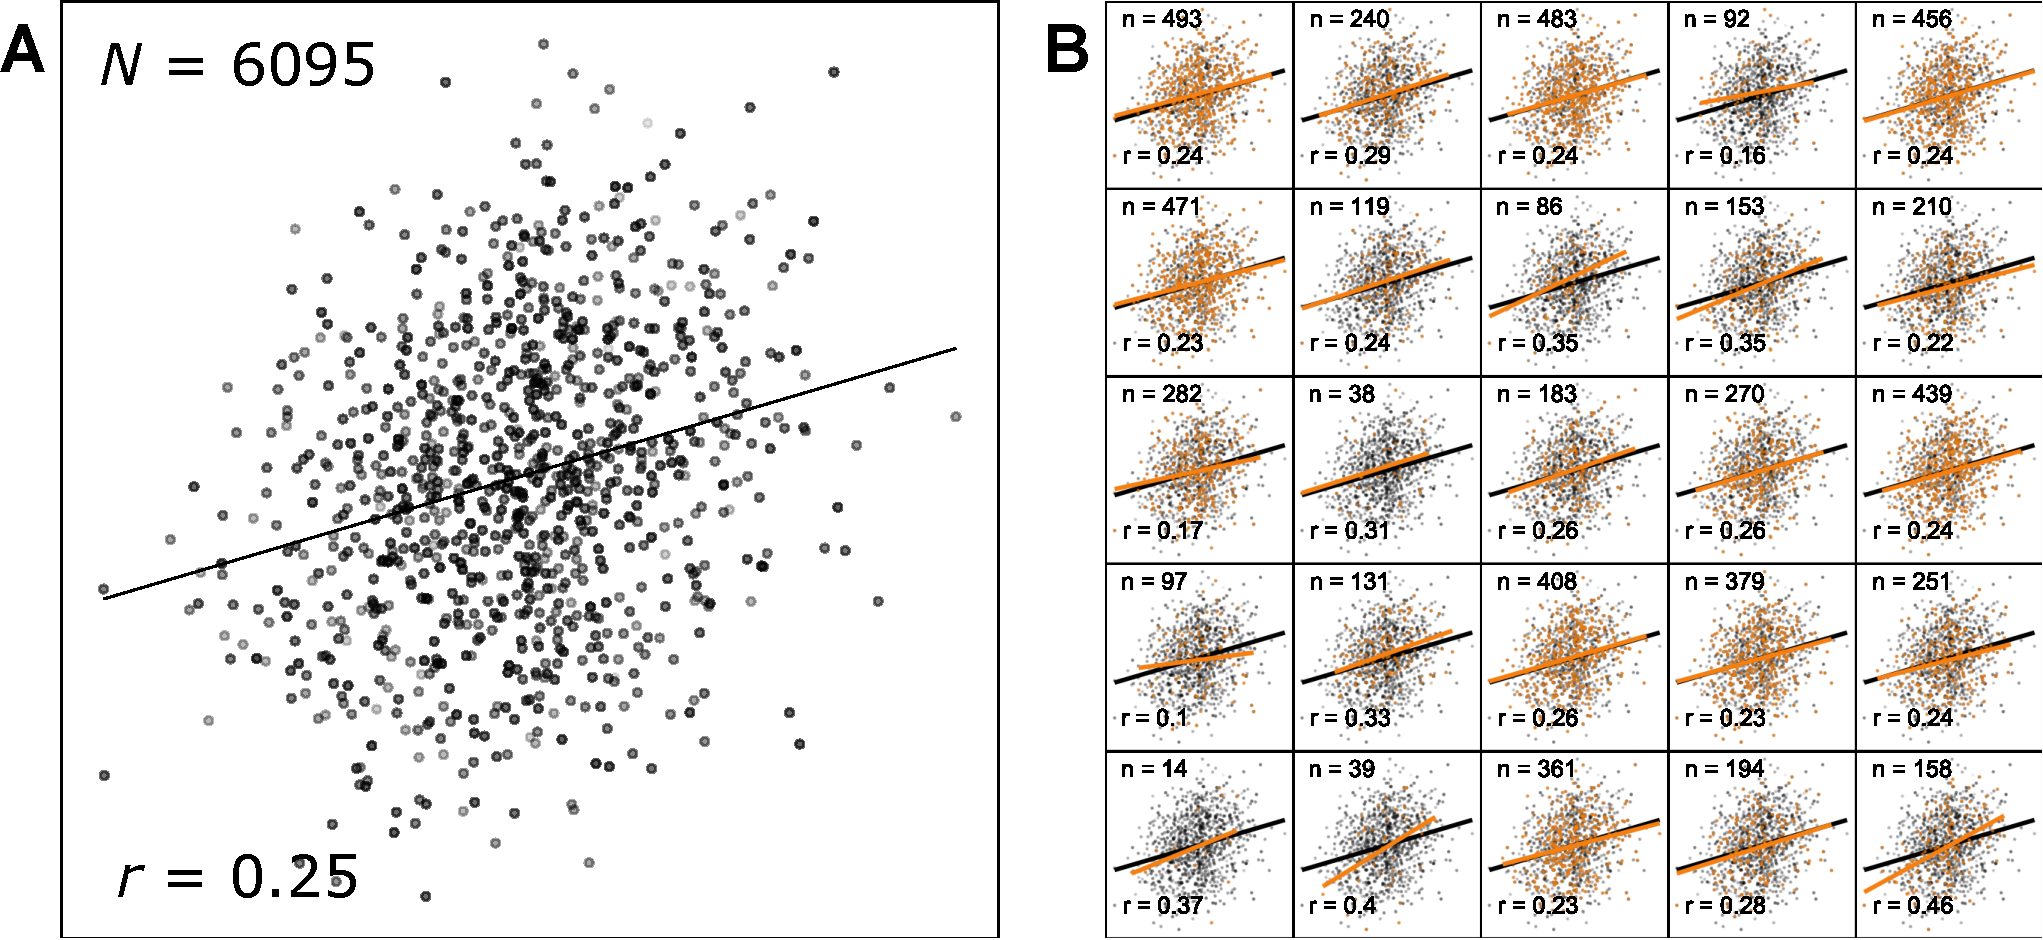
\includegraphics{images/sim_estabilidad.pdf}
\caption{\label{fig:efecto}Simulación de una población hipotética de \emph{N} = 6095 elementos, en la que dos variables se correlacionan positivamente (\emph{r} = 0.25). \textbf{A.} Simulación de la población y correlación entre dos variables. \textbf{B.} 25 muestras aleatorias de diferentes tamaños (\emph{n}) de esa población, y la correlación encontrada en cada una (\emph{r}). En naranja se resaltan los elementos seleccionados aleatoriamente y la correlación encontrada en cada muestra, superpuestos sobre el total de la población y la correlación real (en negro, como referencia).}
\end{figure}

Ahora imagina que tú quieres establecer esa correlación real (\(r\) = 0.25), pero no la conoces, y no tienes acceso a la población completa de 6095 elementos. Tu mejor apuesta es tomar una muestra aleatoria, que en principio tendería a darte un resultado \emph{similar} al real. En el panel \textbf{B} hay 25 muestra aleatorias de esos 6095 elementos, y en cada una se reporta tanto en tamaño de la muestra (\emph{n}, que va desde una muestra muy pequeña de apenas 14 observaciones, hasta una muy respetable de 493), como la correlación encontrada en esa muestra (\emph{r}, que va desde 0.10 hasta 0.46).

Entre las 25 muestra aleatorias de nuestra población (Fig. \ref{fig:efecto}B), hay varias que encuentran una correlación similar a la real (que, como es simulada, sabemos que es exactamente de \(r\) = 0.25), pero hay otras que se alejan bastante. Analiza detalladamente esos resultados y trata de ver si las que más de alejan (estando por debajo o por encima de 0.25), tienen algo en común.

Si miras con cuidado, verás algo claro: las muestras más grandes tienden a encontrar resultados similares al de nuestra población simulada (\(r\) = 0.25). Sin embargo, las muestra pequeñas son menos confiables: aunque algunas muestras pequeñas encuentran correlaciones muy cercanas a la real, otras se alejan mucho. Para ilustrar esto, voy a graficar la correlación encontrada en cada muestra, y cómo se asocia con su tamaño de muestra (Fig. \ref{fig:dist-sim}).

\begin{figure}

{\centering 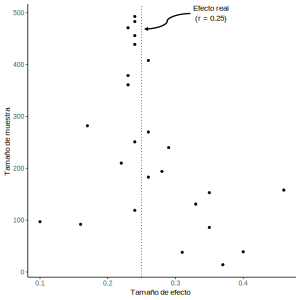
\includegraphics{images/dist-sim} 

}

\caption{Relación entre el efecto encontrado (eje $X$) y el tamaño de muestra (eje $Y$) en 25 muestras aleatorias de una población simulada donde la correlación entre las variables es de $r$ = 0.25. Mientras que las muestras grandes (arriba) son confiables y tienden a encontrar resultados similares al del efeto real, muestras pequeñas (abajo)son menos confiables y puyeden producir estimaciones del efecto que se alejan mucho del real.}\label{fig:dist-sim}
\end{figure}

\hypertarget{quuxe9-es-un-meta-anuxe1lisis-y-por-quuxe9-es-importante}{%
\subsection{¿Qué es un meta-análisis y por qué es importante?}\label{quuxe9-es-un-meta-anuxe1lisis-y-por-quuxe9-es-importante}}

De manera más general, se puede entender así: aunque hay técnicas de muestreo que tienden a hacer que las muestras se \emph{parezcan} más a la población, cada muestra tiene características particulares que conducen a resultados diferentes. Entonces, cuando debemos hacer inferencia con base en muestras porque no podemos tener acceso a la población entera, ¿cómo podemos saber cuál es el efecto real si cada estudio obtiene un resultado distinto?

Una herramienta útil para abordar este problema es el meta-análisis, que es una técnica estadística que nos permite obtener una estimación más precisa del efecto \emph{real} de la correlación. Por supuesto, la palabra clave acá es \emph{estimación}, pues aunque el efecto real es algo que rara vez podremos determinar con absoluta certeza, sí es algo que podemos acercarnos a conocer.

El meta-análisis se puede entender como una especie \emph{promediación} de los efectos encontrados en diversos estudios, dando mayor peso a estudios que tienen más credibilidad (es decir, mayor probabilidad de mostrar un resultado cercano a la verdad). ¿Cómo se hace esto? Como se ve en la Figura \ref{fig:dist-sim}, el tamaño de una muestra afecta la confiabilidad de un resultado.

Para decirlo de manera más técnica, el tamaño de muestra afecta el poder estadístico así como el error en la estimación del efecto (\protect\hyperlink{ref-leongomezAnalisisPoderEstadistico2020}{Leongómez, 2020a}, \protect\hyperlink{ref-leongomezPoderRvid2020}{2020b}); entre mayor sea una muestra, mayor será el poder estadístico y menor tenderá a ser su variación con respecto al efecto real (en últimas, muestras más grandes tienden a parecerse más a la población de la que provienen y por tanto son más confiables). Por esto, podemos usar estas medidas como indicadores de la credibilidad del efecto encontrado por un estudio.

\hypertarget{sesgos-de-publicaciuxf3n}{%
\subsection{Sesgos de publicación}\label{sesgos-de-publicaciuxf3n}}

Sin embargo, además de las diferencias que pueda tener cada estudio debido a las peculiaridades y tamaño de su muestra, con frecuencia al hacer meta-análisis nos enfrentamos a un riesgo más sutil y menos predecible: los sesgos de publicación.

Los sesgos de publicación son una amenaza importante para la integridad de la investigación científica. Se refieren a la tendencia de los investigadores y editores de revistas a no publicar estudios que no encuentran un efecto significativo o que muestran resultados contrarios a las hipótesis de sus autores. Estos sesgos pueden afectar a todas las áreas de la investigación, pasando por ejemplo por la medicina, la psicología y la biología (e.g., \protect\hyperlink{ref-baker500ScientistsLift2016}{Baker, 2016}; \protect\hyperlink{ref-kleinManyLabsInvestigating2018}{Klein et al., 2018}).

Como resultado, los estudios publicados pueden no ser representativos de la verdadera relación entre las variables que se están investigando, lo que puede llevar a conclusiones erróneas y a decisiones equivocadas, incluyendo áreas tan críticas como la práctica clínica y la toma de decisiones políticas, por ejemplo.

Imagina, por ejemplo, que frente a un efecto estudiado se publicaron preferentemente estudios que encontraron una correlación positiva y significativa, mientras que otros estudios ---que no encontraron una correlación o encontraron una correlación negativa--- tendieron a no ser publicados por los autores, o a ser rechazados por editores. Al hacer un meta-análisis de los estudios publicados, nuestra estimación del efecto \emph{real} estaría sesgada, sobre-estimando el efecto (Fig. \ref{fig:teoria-meta}).

\begin{figure}
\centering
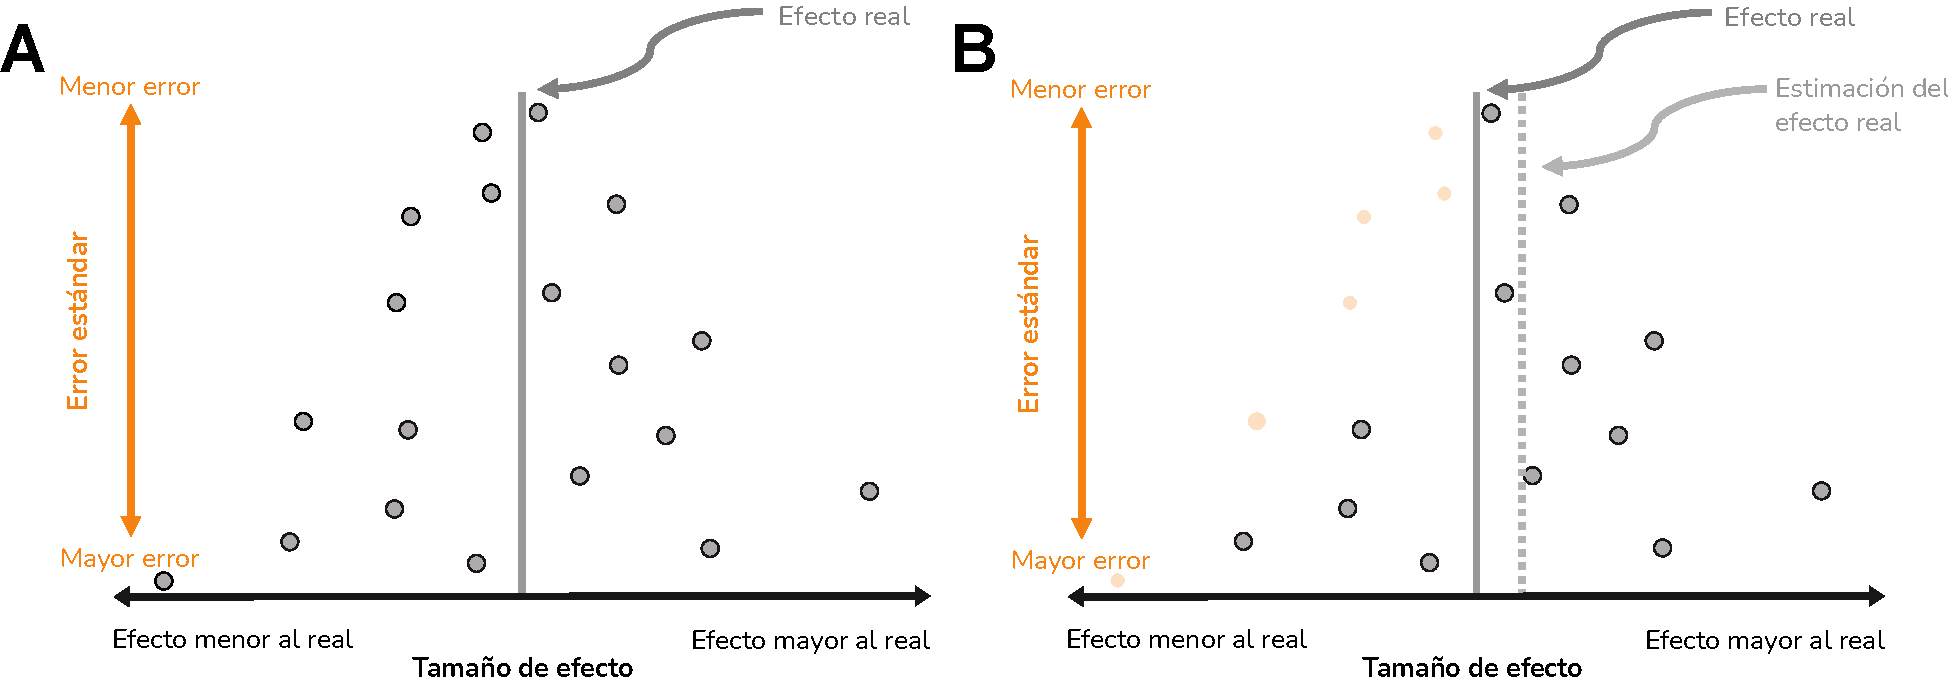
\includegraphics{images/Teoria-meta_FIN.pdf}
\caption{\label{fig:teoria-meta}Ejemplo hipotético de distribución de resultados de diferentes estudios (puntos grises) en relación a un efecto real (línea gris vertical). Los estudios realizados con diferentes muestras tienden a estar a ambos lados del efecto real (efectos mayores al real a la derecha y efectos menores a la izquierda). Sin embargo, entre mayor sea la muestra (arriba) los estudios tienden a estar más cerca del efecto real (tienen menor error), pero estudios con muestras pequeñas (abajo) son más variables (y en promedio tienen mayor error), y pueden tener efectos muy alejados del efecto real. Esto forma una especie de triángulo simétrico, con el efecto real en el centro. Esta idea, aunque simplificada en este ejemplo, está en la base misma del meta-análisis, y es similar a lo que comúnmente se representa en un diagrama de embudo (\textit{funnel plot}). \textbf{A.} Distribución cuando no hay sesgo de publicación. \textbf{B.} Distribución de resultados en el caso hipotético de que algunos estudios con efectos bajos no fueran publicados (puntos naraja claros). Debido a esto, un meta-análisis estaría sesgado, y el efecto estimado (línea gris punteada) sería mayor al efecto real (línea gris sólida).}
\end{figure}

Por suerte, existen técnicas poderosas para buscar evidencia de sesgos de publicación en los estudios incluidos en un meta-análisis, y hacer estimaciones corregidas del efecto \emph{real} que tengan estos sesgos en cuenta para hacer estimaciones más precisas.

\hypertarget{motivaciuxf3n}{%
\subsection{Motivación}\label{motivaciuxf3n}}

Teniendo en cuenta la importancia de éstas técnicas, y la relativa escasez de material de buena calidad en español, accesible tanto para estudiantes como para investigadores curtidos, he decidido hacer esta guía. He incluido información actualizada, soportada siempre en fuentes de alta calidad que pueden ser consultadas por las personas que quieran profundizar en cada tema.

A lo largo del documento daré ejemplos e instrucciones precisas de cómo hacer un meta-análisis básico en R (sección \ref{meta-cor}), incluyendo cómo hacer análisis de heterogeneidad (sección \ref{heterog-inf}) y diagnósticos de influencia (sección \ref{diag-inf}), creación de gráficos de bosque (\emph{forest plots}; sección \ref{forest-inf}) y gráficos de embudo (\emph{funnel plots}; sección \ref{funnel-inf}), así como estrategias para detectar posibles sesgos de publicación (secciones \ref{sesgo-pub} y \ref{todas-combinaciones}), y para determinar el poder estadístico de un meta-análisis (sección \ref{poder-inf}). Finalmente, mostraré técnicas de meta-regresión para investigar los factores que pueden influir en los resultados de los estudios incluidos en un meta-análisis (sección \ref{met-moderation}).

Adicionalmente, he incluido algunos apéndices, donde encontrarás información concreta sobre otras rutas alternativas para hacer meta-análisis en R (Apéndice \hyperlink{apendice-alt}{A}), incluyendo instrucciones para hacer una curva de valores \(p\) (\emph{p-curve}; Apéndice \hyperlink{p-curve}{A1}), así como la manera correcta de citar paquetes de R (Apéndice \hyperlink{paquetes-cit}{B}) y, con fines de garantizar la reproducibilidad de éste documento, una lista de los paquetes usados para la creación de ésta guía, con sus respectivas versiones (Apéndice \hyperlink{paquetes-list}{C}).

\begin{center}\rule{0.5\linewidth}{0.5pt}\end{center}

\hypertarget{base-de-datos-de-ejemplo}{%
\section{Base de datos de ejemplo}\label{base-de-datos-de-ejemplo}}

A lo largo de esta guía usaré la base de datos \texttt{dat.molloy2014}, tomada de Molloy et al. (\protect\hyperlink{ref-molloy2013}{2013}). Esta base de datos viene incluida con el paquete \texttt{metafor} de R.

Básicamente, Molloy et al. (\protect\hyperlink{ref-molloy2013}{2013}) estudiaron si existe una asociación entre la escrupulosidad (\emph{conscientiousness}\footnote{En el contexto de los rasgos de personalidad, la dimensión de la \emph{escrupulosidad} (también llamada conciencia o ``voluntad de logro''), se refiere al auto-control, incluyendo la planificación y ejecución de tareas. Para una definición detallada del concepto de escrupulosidad en este contexto, ver John \& Srivastava (\protect\hyperlink{ref-johnBigFiveTrait1999}{1999}).}) y la adherencia a la medicación. En otras palabras, ¿las personas más \emph{escrupulosas} tienden a cumplir más con la medicación prescrita?

Primero, debemos cargar los principales paquetes que usaré a lo largo de esta guía: \texttt{metafor} (\protect\hyperlink{ref-viechtbauer2010}{Viechtbauer, 2010}) y \texttt{metaviz} (\protect\hyperlink{ref-KossmeierMetaviz}{Kossmeier et al., 2020}) para hacer e ilustrar los resultados del meta-análisis, así como \texttt{dplyr} (\protect\hyperlink{ref-WickhamDplyr2021}{Wickham et al., 2021}), \texttt{magrittr} (\protect\hyperlink{ref-magrittrcite}{Bache \& Wickham, 2022}) y \texttt{forecats} (\protect\hyperlink{ref-Wickhamforcats2022}{Wickham, 2022}) para manipular y organizar la base de datos.

\begin{Shaded}
\begin{Highlighting}[]
\FunctionTok{library}\NormalTok{(metafor)}
\FunctionTok{library}\NormalTok{(metaviz)}
\FunctionTok{library}\NormalTok{(dplyr)}
\FunctionTok{library}\NormalTok{(magrittr)}
\FunctionTok{library}\NormalTok{(forcats)}
\end{Highlighting}
\end{Shaded}

Como ya hemos cargado el paquete \texttt{metafor}, ya podemos cargar la base de datos \texttt{dat.molloy2014}. En éste caso, para poder \emph{llamarla} cuando sea necesario, la asignaré a un objeto que llamaré simplemente \texttt{dat}.

\begin{Shaded}
\begin{Highlighting}[]
\NormalTok{dat }\OtherTok{\textless{}{-}} \FunctionTok{get}\NormalTok{(}\FunctionTok{data}\NormalTok{(dat.molloy2014))}
\end{Highlighting}
\end{Shaded}

Tras asignar la base de datos a este objeto (\texttt{dat}), la base de datos se puede ver como \emph{output}\footnote{En R y otros lenguajes de programación, se llama ``\emph{output}'' a la \emph{salida} o resultado visible de una función o proceso, en este caso en la consola (que en RStudio es normalmente el panel que está a la izquierda en la parte inferior).} en la consola de R sencillamente usando como comando el nombre que le dimos al objeto al que lo asignamos (en este caso, \texttt{dat}).

\begin{Shaded}
\begin{Highlighting}[]
\NormalTok{dat}
\end{Highlighting}
\end{Shaded}

\begin{ROut}{Consola de R: Output~\thetcbcounter}
                \begin{footnotesize}
                \begin{verbatim}                authors year  ni     ri controls          design   a_measure
1      Axelsson et al. 2009 109  0.187     none cross-sectional self-report
2      Axelsson et al. 2011 749  0.162     none cross-sectional self-report
3         Bruce et al. 2010  55  0.340     none     prospective       other
4   Christensen et al. 1999 107  0.320     none cross-sectional self-report
5  Christensen & Smith 1995  72  0.270     none     prospective       other
6         Cohen et al. 2004  65  0.000     none     prospective       other
7       Dobbels et al. 2005 174  0.175     none cross-sectional self-report
8        Ediger et al. 2007 326  0.050 multiple     prospective self-report
9         Insel et al. 2006  58  0.260     none     prospective       other
10       Jerant et al. 2011 771  0.010 multiple     prospective       other
11        Moran et al. 1997  56 -0.090 multiple     prospective       other
12   O'Cleirigh et al. 2007  91  0.370     none     prospective self-report
13       Penedo et al. 2003 116  0.000     none cross-sectional self-report
14        Quine et al. 2012 537  0.150     none     prospective self-report
15      Stilley et al. 2004 158  0.240     none     prospective       other
16 Wiebe & Christensen 1997  65  0.040     none     prospective       other
   c_measure meanage quality
1      other   22.00       1
2        NEO   53.59       1
3        NEO   43.36       2
4      other   41.70       1
5        NEO   46.39       2
6        NEO   41.20       2
7        NEO   52.30       1
8        NEO   41.00       3
9      other   77.00       2
10       NEO   78.60       3
11       NEO   57.20       2
12       NEO   37.90       2
13       NEO   39.20       1
14     other   69.00       2
15       NEO   46.20       3
16       NEO   56.00       1
 \end{verbatim}
                \end{footnotesize}
                \end{ROut}

\hypertarget{variables-inf}{%
\subsection{Variables de la base de datos}\label{variables-inf}}

Por favor mira la base de datos, y familiarízate con sus columnas. ¿Qué información contiene cada variable? Explicaré cada una a continuación.

Primero, hay unas columnas que contienen información absolutamente necesaria para poder hacer un meta-análisis:

\begin{itemize}
\item
  \texttt{authors}: los autores de cada estudio a meta-analizar
\item
  \texttt{year}: año de publicación de cada estudio
\item
  \texttt{ni}: tamaño de muestra de cada estudio
\item
  \texttt{ri}: coeficiente de correlación de Pearson de cada estudio
\end{itemize}

Esas son las variables más importantes y son necesarias para hacer un meta-análisis de correlación simple: alguna columna o columnas con información que permita identificar cada estudio (en este caso \texttt{authors} y \texttt{year}), una columna con el tamaño de muestra de cada estudio (en este caso, \texttt{ni}), y finalmente una columna con los coeficientes de correlación (en este caso la columna \texttt{ri}). Si tu meta-análisis no requiere moderadores, con una estructura como esta sería suficiente.

Después hay unas columnas que contienen variables específicas para este este ejemplo, y que son una serie de posibles moderadores que agrupan características de los estudios a meta-analizar:

\begin{itemize}
\item
  \texttt{controls}: cantidad de variables controladas (``\texttt{none}'': ninguna o ``\texttt{multiple}'': múltiples)
\item
  \texttt{design}: si se utilizó un diseño transversal (``\texttt{cross-section}'') o prospectivo (``\texttt{prospective}'') (para más información acerca de estos tipos de diseño, ver por ejemplo \protect\hyperlink{ref-Manterola2019}{Manterola et al., 2019})
\item
  \texttt{a\_measure}: tipo de medida de adherencia (``\texttt{self-report}'': autoinforme u ``\texttt{other}'': otro tipo de medida más \emph{objetivo})
\item
  \texttt{c\_measure}: tipo de medida de escrupulosidad (si se midió con alguna versión del inventario de personalidad NEO o con alguna otra escala)
\item
  \texttt{meanage}: edad promedio de la muestra de cada estudio
\item
  \texttt{quality}: calidad metodológica (la calidad metodológica fue calificada por los autores del meta-análisis en una escala de 1 a 4, donde las puntuaciones más altas indican una mayor calidad; para información respecto a cómo se obtuvo esta puntuación, ver el artículo original de Molloy et al. (\protect\hyperlink{ref-molloy2013}{2013}).
\end{itemize}

Por supuesto, el \emph{output} de la consola no es la forma más clara de ver la base de datos, pero para una versión más legible, se puede usar la función \texttt{View}, y el nombre de la base de datos o tabla como argumento (en este caso \texttt{View(dat)}). Sin embargo, de aquí en adelante mostraré algunas tablas en un formato de impresión (y no como sale en la consola de R), para que sean más fáciles de leer.

Voy a volver a cargar la base de datos (sobrescribiendo el objeto \texttt{dat}), para organizarla un poco mejor. Primero, agregaré una nueva columna llamada \texttt{study\_id}, en la que numeraré los estudios del 1 al 16, lo que será útil para identificar cada estudio en algunas gráficas y análisis. Después, reorganizaré las columnas para que \texttt{study\_id} sea la primera, en vez de la última columna. Finalmente, las columnas de variables que son factores (\texttt{controls}, \texttt{design}, \texttt{a\_measure}, \texttt{c\_measure} y \texttt{quality}), pueden ser definidas como tal, para evitar pasos adicionales más adelante. En este caso, además, voy a reorganizar los niveles de la variable \texttt{controls} (primero \texttt{none} y después \texttt{multiple}); esto, aunque no es un paso necesario, puede ayudar con la interpretación de resultados.

\begin{Shaded}
\begin{Highlighting}[]
\NormalTok{dat }\OtherTok{\textless{}{-}} \FunctionTok{get}\NormalTok{(}\FunctionTok{data}\NormalTok{(dat.molloy2014)) }\SpecialCharTok{\%\textgreater{}\%}
  \FunctionTok{mutate}\NormalTok{(}\AttributeTok{study\_id =} \DecValTok{1}\SpecialCharTok{:}\DecValTok{16}\NormalTok{)  }\SpecialCharTok{\%\textgreater{}\%} \CommentTok{\# crear columna \textquotesingle{}study\_id\textquotesingle{} y agregar números del 1 al 16}
  \FunctionTok{select}\NormalTok{(study\_id, authors}\SpecialCharTok{:}\NormalTok{quality) }\SpecialCharTok{\%\textgreater{}\%} \CommentTok{\# mover \textquotesingle{}study\_id\textquotesingle{} como primera columna}
  \FunctionTok{mutate\_at}\NormalTok{(}\FunctionTok{c}\NormalTok{(}\StringTok{"controls"}\NormalTok{, }\CommentTok{\# transformar variables relevantes en factores}
              \StringTok{"design"}\NormalTok{,}
              \StringTok{"a\_measure"}\NormalTok{,}
              \StringTok{"c\_measure"}\NormalTok{,}
              \StringTok{"quality"}\NormalTok{), }
\NormalTok{            as.factor) }\SpecialCharTok{\%\textgreater{}\%} 
  \FunctionTok{mutate}\NormalTok{(}\AttributeTok{controls =} \FunctionTok{fct\_relevel}\NormalTok{(controls, }\CommentTok{\# reorganizar niveles de la variable \textquotesingle{}controls\textquotesingle{}}
                                \StringTok{"none"}\NormalTok{, }\StringTok{"multiple"}\NormalTok{))  }
\end{Highlighting}
\end{Shaded}

Con esto, la base de datos tiene ahora la siguiente estructura (Tabla \ref{tab:estructuramod}):

\begin{table}[H]

\caption{\label{tab:estructuramod}Estructura de la base de datos con estudios numerados}
\centering
\resizebox{\linewidth}{!}{
\begin{tabular}[t]{rlrrrllllrl}
\toprule
study\_id & authors & year & ni & ri & controls & design & a\_measure & c\_measure & meanage & quality\\
\midrule
1 & Axelsson et al. & 2009 & 109 & 0.187 & none & cross-sectional & self-report & other & 22.00 & 1\\
2 & Axelsson et al. & 2011 & 749 & 0.162 & none & cross-sectional & self-report & NEO & 53.59 & 1\\
3 & Bruce et al. & 2010 & 55 & 0.340 & none & prospective & other & NEO & 43.36 & 2\\
4 & Christensen et al. & 1999 & 107 & 0.320 & none & cross-sectional & self-report & other & 41.70 & 1\\
5 & Christensen \& Smith & 1995 & 72 & 0.270 & none & prospective & other & NEO & 46.39 & 2\\
6 & Cohen et al. & 2004 & 65 & 0.000 & none & prospective & other & NEO & 41.20 & 2\\
7 & Dobbels et al. & 2005 & 174 & 0.175 & none & cross-sectional & self-report & NEO & 52.30 & 1\\
8 & Ediger et al. & 2007 & 326 & 0.050 & multiple & prospective & self-report & NEO & 41.00 & 3\\
9 & Insel et al. & 2006 & 58 & 0.260 & none & prospective & other & other & 77.00 & 2\\
10 & Jerant et al. & 2011 & 771 & 0.010 & multiple & prospective & other & NEO & 78.60 & 3\\
11 & Moran et al. & 1997 & 56 & -0.090 & multiple & prospective & other & NEO & 57.20 & 2\\
12 & O'Cleirigh et al. & 2007 & 91 & 0.370 & none & prospective & self-report & NEO & 37.90 & 2\\
13 & Penedo et al. & 2003 & 116 & 0.000 & none & cross-sectional & self-report & NEO & 39.20 & 1\\
14 & Quine et al. & 2012 & 537 & 0.150 & none & prospective & self-report & other & 69.00 & 2\\
15 & Stilley et al. & 2004 & 158 & 0.240 & none & prospective & other & NEO & 46.20 & 3\\
16 & Wiebe \& Christensen & 1997 & 65 & 0.040 & none & prospective & other & NEO & 56.00 & 1\\
\bottomrule
\multicolumn{11}{l}{\rule{0pt}{1em}\textit{Nota:} Datos tomados de Molloy et al. (2013).}\\
\end{tabular}}
\end{table}

\hypertarget{preparaciuxf3n-de-los-datos-transformaciuxf3n-de-coeficientes-r-de-pearson-a-z-de-fisher}{%
\subsection{\texorpdfstring{Preparación de los datos: transformación de coeficientes \emph{r} de Pearson a \emph{z} de Fisher}{Preparación de los datos: transformación de coeficientes r de Pearson a z de Fisher}}\label{preparaciuxf3n-de-los-datos-transformaciuxf3n-de-coeficientes-r-de-pearson-a-z-de-fisher}}

Los coeficientes de Pearson no se distribuyen normalmente, lo que podría llevar a calcular varianzas incorrectas, especialmente cuando se trata de correlaciones con tamaños de muestra pequeño (\protect\hyperlink{ref-shadishCombiningEstimatesEffect2009}{Shadish \& Haddock, 2009}). Por esto, lo mejor es transformar los coeficientes \emph{r} de Pearson a \emph{z} de Fisher (\protect\hyperlink{ref-fisherFrequencyDistributionValues1915}{1915}), que no tienen este problema\footnote{Para decirlo de manera más precisa, el problema es que la distribución del coeficiente de correlación de Pearson (\emph{r}), es muy sesgada cuando se trata de variables altamente correlacionadas (positiva, o negativamente). Esto dificulta la estimación de los intervalos de confianza y por tanto la aplicación de las pruebas de significación para coeficientes \emph{r} (e.g., \protect\hyperlink{ref-shadishCombiningEstimatesEffect2009}{Shadish \& Haddock, 2009}). La transformación de Fisher de valores \emph{r} a \emph{z} ---que es la \href{https://es.wikipedia.org/wiki/Tangente_hiperb\%C3\%B3lica}{tangente hiperbólica inversa} de \emph{r}--- resuelve este problema, pues los coeficientes \emph{z} tienen una distribución aproximadamente normal, y una varianza estable a lo largo de diferentes valores posibles de \emph{r} (para una demostración en español, ver \protect\hyperlink{ref-sanchez-brunoTransformacionFisherPara2005}{Sánchez-Bruno \& Borges del Rosal, 2005}).}.

Para transformar los coeficientes \emph{r} de Pearson a coeficientes \emph{z} de Fisher, usaré la función \texttt{escalc} del paquete \texttt{metafor}, que sirve para calcular diversos tamaños de efecto que se utilizan comúnmente en meta-análisis. Los argumentos que requiere esta función, además del tipo de transformación a realizar (en este caso \texttt{measure\ =\ "ZCOR"}), son los coeficientes de correlación (\texttt{ri}), el tamaño de muestra de cada correlación (\texttt{ni}), y la base de datos que contiene estos valores (\texttt{data}). En nuestro caso, las columnas donde están estos valores, tienen los mismos nombres (\texttt{ri}, \texttt{ni}). En este ejemplo, asignaré el resultado de esta función al mismo objeto \texttt{dat}, que contiene la base de datos, para sobrescribirlo y no crear objetos adicionales.

\begin{Shaded}
\begin{Highlighting}[]
\NormalTok{dat }\OtherTok{\textless{}{-}} \FunctionTok{escalc}\NormalTok{(}\AttributeTok{measure =} \StringTok{"ZCOR"}\NormalTok{, }\AttributeTok{ri =}\NormalTok{ ri, }\AttributeTok{ni =}\NormalTok{ ni, }\AttributeTok{data =}\NormalTok{ dat)}
\end{Highlighting}
\end{Shaded}

Esta función agrega dos nuevas variables: \texttt{yi}, que es el tamaño de efecto (en valores \emph{z} de Fisher), y \texttt{vi} que es la varianza (Tabla \ref{tab:estructuramod2}).

\begin{table}[H]

\caption{\label{tab:estructuramod2}Estructura de la base de datos, con transformación de los r de Pearon a z de Fisher}
\centering
\resizebox{\linewidth}{!}{
\begin{tabular}[t]{rlrrrllllrl>{}r>{}r}
\toprule
study\_id & authors & year & ni & ri & controls & design & a\_measure & c\_measure & meanage & quality & yi & vi\\
\midrule
1 & Axelsson et al. & 2009 & 109 & 0.187 & none & cross-sectional & self-report & other & 22.00 & 1 & \cellcolor[HTML]{f68212}{0.1892266} & \cellcolor[HTML]{f68212}{0.0094340}\\
2 & Axelsson et al. & 2011 & 749 & 0.162 & none & cross-sectional & self-report & NEO & 53.59 & 1 & \cellcolor[HTML]{f68212}{0.1634399} & \cellcolor[HTML]{f68212}{0.0013405}\\
3 & Bruce et al. & 2010 & 55 & 0.340 & none & prospective & other & NEO & 43.36 & 2 & \cellcolor[HTML]{f68212}{0.3540925} & \cellcolor[HTML]{f68212}{0.0192308}\\
4 & Christensen et al. & 1999 & 107 & 0.320 & none & cross-sectional & self-report & other & 41.70 & 1 & \cellcolor[HTML]{f68212}{0.3316471} & \cellcolor[HTML]{f68212}{0.0096154}\\
5 & Christensen \& Smith & 1995 & 72 & 0.270 & none & prospective & other & NEO & 46.39 & 2 & \cellcolor[HTML]{f68212}{0.2768638} & \cellcolor[HTML]{f68212}{0.0144928}\\
6 & Cohen et al. & 2004 & 65 & 0.000 & none & prospective & other & NEO & 41.20 & 2 & \cellcolor[HTML]{f68212}{0.0000000} & \cellcolor[HTML]{f68212}{0.0161290}\\
7 & Dobbels et al. & 2005 & 174 & 0.175 & none & cross-sectional & self-report & NEO & 52.30 & 1 & \cellcolor[HTML]{f68212}{0.1768200} & \cellcolor[HTML]{f68212}{0.0058480}\\
8 & Ediger et al. & 2007 & 326 & 0.050 & multiple & prospective & self-report & NEO & 41.00 & 3 & \cellcolor[HTML]{f68212}{0.0500417} & \cellcolor[HTML]{f68212}{0.0030960}\\
9 & Insel et al. & 2006 & 58 & 0.260 & none & prospective & other & other & 77.00 & 2 & \cellcolor[HTML]{f68212}{0.2661084} & \cellcolor[HTML]{f68212}{0.0181818}\\
10 & Jerant et al. & 2011 & 771 & 0.010 & multiple & prospective & other & NEO & 78.60 & 3 & \cellcolor[HTML]{f68212}{0.0100003} & \cellcolor[HTML]{f68212}{0.0013021}\\
11 & Moran et al. & 1997 & 56 & -0.090 & multiple & prospective & other & NEO & 57.20 & 2 & \cellcolor[HTML]{f68212}{-0.0902442} & \cellcolor[HTML]{f68212}{0.0188679}\\
12 & O'Cleirigh et al. & 2007 & 91 & 0.370 & none & prospective & self-report & NEO & 37.90 & 2 & \cellcolor[HTML]{f68212}{0.3884231} & \cellcolor[HTML]{f68212}{0.0113636}\\
13 & Penedo et al. & 2003 & 116 & 0.000 & none & cross-sectional & self-report & NEO & 39.20 & 1 & \cellcolor[HTML]{f68212}{0.0000000} & \cellcolor[HTML]{f68212}{0.0088496}\\
14 & Quine et al. & 2012 & 537 & 0.150 & none & prospective & self-report & other & 69.00 & 2 & \cellcolor[HTML]{f68212}{0.1511404} & \cellcolor[HTML]{f68212}{0.0018727}\\
15 & Stilley et al. & 2004 & 158 & 0.240 & none & prospective & other & NEO & 46.20 & 3 & \cellcolor[HTML]{f68212}{0.2447741} & \cellcolor[HTML]{f68212}{0.0064516}\\
16 & Wiebe \& Christensen & 1997 & 65 & 0.040 & none & prospective & other & NEO & 56.00 & 1 & \cellcolor[HTML]{f68212}{0.0400214} & \cellcolor[HTML]{f68212}{0.0161290}\\
\bottomrule
\multicolumn{13}{l}{\rule{0pt}{1em}\textit{Nota:} Las nuevas columnas creadas usando la función \texttt{escalc} 
           (\texttt{yi} como tamaño de efecto y \texttt{vi} como varianza) están 
           resaltadas en naranja}\\
\end{tabular}}
\end{table}

\begin{center}\rule{0.5\linewidth}{0.5pt}\end{center}

\hypertarget{meta-cor}{%
\section{Cómo hacer el meta-análisis}\label{meta-cor}}

Para hacer el meta-análisis, usaré la función \texttt{rma} del paquete \texttt{metafor}. Esta función requiere especificar los tamaños de efecto (\texttt{yi}) y varianzas (\texttt{vi}) de los estudios a meta-analizar. En nuestro caso, las columnas donde están estos valores, tienen los mismos nombres (\texttt{yi}, \texttt{vi}). Asignaré los resultados del meta-análisis a un nuevo objeto llamado \texttt{res}.

\begin{Shaded}
\begin{Highlighting}[]
\NormalTok{res }\OtherTok{\textless{}{-}} \FunctionTok{rma}\NormalTok{(}\AttributeTok{yi =}\NormalTok{ yi, }\AttributeTok{vi =}\NormalTok{ vi, }\AttributeTok{data =}\NormalTok{ dat)}
\end{Highlighting}
\end{Shaded}

Los resultados, son los siguientes:

\begin{Shaded}
\begin{Highlighting}[]
\NormalTok{res}
\end{Highlighting}
\end{Shaded}

\begin{ROut}{Consola de R: Output~\thetcbcounter}
                \begin{footnotesize}
                \begin{verbatim} 
Random-Effects Model (k = 16; tau^2 estimator: REML)

tau^2 (estimated amount of total heterogeneity): 0.0081 (SE = 0.0055)
tau (square root of estimated tau^2 value):      0.0901
I^2 (total heterogeneity / total variability):   61.73%
H^2 (total variability / sampling variability):  2.61

Test for Heterogeneity:
Q(df = 15) = 38.1595, p-val = 0.0009

Model Results:

estimate      se    zval    pval   ci.lb   ci.ub      
  0.1499  0.0316  4.7501  <.0001  0.0881  0.2118  *** 

---
Signif. codes:  0 '***' 0.001 '**' 0.01 '*' 0.05 '.' 0.1 ' ' 1
 \end{verbatim}
                \end{footnotesize}
                \end{ROut}

\hypertarget{meta-interp}{%
\subsection{Interpretación de los resultados del meta-análisis}\label{meta-interp}}

Vamos a analizar estos resultados de la consola de R por partes:

Primero, nos confirman que ajustamos un modelo con efectos aleatorios (\texttt{Random-Effects\ Model}), a partir de 16 estudios (\texttt{k\ =\ 16}), y que para estimar \(\tau^2\) (tau cuadrado) usamos el método de \textbf{máxima verosimilitud restringida}\footnote{Hay varios métodos disponibles como estimador, además de \textbf{máxima verosimilitud restringida} (REML). Sin embargo, si tienes dudas, REML es una buena opción. Cada método tiene ventajas y desventajas que, si tienes interés en mirar, están descritas en la \href{https://www.rdocumentation.org/packages/metafor/versions/2.4-0/topics/rma.uni}{documentación} de la función \texttt{rma}.} (\texttt{tau\^{}2\ estimator:\ REML}), que se designa como \emph{REML} por sus siglas en inglés .

Posteriormente, nos provee los valores de una serie de estimadores de heterogeneidad:

\begin{itemize}
\item
  \(\tau^2\): \texttt{tau\^{}2\ (estimated\ amount\ of\ total\ heterogeneity):\ 0.0081\ (SE\ =\ 0.0055)}
\item
  \(\tau\): \texttt{tau\ (square\ root\ of\ estimated\ tau\^{}2\ value):\ 0.0901}
\item
  \(I^2\): \texttt{I\^{}2\ (total\ heterogeneity\ /\ total\ variability):\ 61.73\%}, y
\item
  \(H^2\): \texttt{H\^{}2\ (total\ variability\ /\ sampling\ variability):\ \ 2.61}
\end{itemize}

La tercera parte, reporta otra prueba de heterogeneidad, usando el estadístico \(Q\):

\begin{itemize}
\item
  \texttt{Test\ for\ Heterogeneity:}

  \texttt{Q(df\ =\ 15)\ =\ 38.1595,\ p-val\ =\ 0.0009}
\end{itemize}

De todos estos, los más comúnmente reportados son \(\tau^2\), \(\tau\), \(I^2\) y \(Q\). Cada una de estas medidas tiene ventajas y desventajas, por lo cual tiene sentido reportarlas todas.

\begin{itemize}
\item
  \(I^2\): tiene la ventaja de ser sencillo de interpretar, pues hay criterios generales para heterogeneidad baja, moderada y alta (típicamente 25\%, 50\%, and 75\%, respectivamente). Sin embargo, es muy sensible a los tamaños de muestra de los estudios meta-analizados (por ejemplo, si en tu meta-análisis hay estudios con tamaños de muestra muy grandes, esto va a sesgar tu \(I^2\)).
\item
  \(Q\): aunque no es sensible al tamaño de muestra, es sensible al número de estudios meta-analizados. Tiene la ventaja de ser un test de hipótesis, y como tal, puede ser interpretado a partir de su valor \emph{p}.
\item
  \(\tau^2\): no tiene problemas de sensibilidad a los tamaños de muestra o número de estudios meta-analizados, pero es más difícil de interpretar. \(\tau^2\) es una estimación de la varianza de los tamaños de los efectos reales entre los estudios meta-analizados. Se usa, principalmente, para asignar pesos a cada estudio (para más información, ver \protect\hyperlink{ref-borensteinIdentifyingQuantifyingHeterogeneity2009}{Borenstein et al., 2009}).
\end{itemize}

En nuestro caso, el estadístico \(Q\) sugiere que hay una heterogeneidad significativa en los estudios meta-analizados (\(p\) = 0.0009). \(I^2\), sugiere una heterogeneidad moderada, lo que quiere decir que se estima que más de la mitad (61.73\%) de la varianza se deriva de diferencias en los tamaños de efecto.

Más abajo, el \emph{output} de la consola de R nos muestra los resultados de nuestro meta-análisis (\texttt{Model\ results}); en otras palabras, ¿cuál es el tamaño de efecto de la asociación entre escrupulosidad (\emph{conscientiousness}) y la adherencia a la medicación, según nuestro meta-análisis?

Esta parte nos provee varios resultados:

\begin{itemize}
\item
  \texttt{Estimate\ (0.1499)}: estimado de la correlación entre escrupulosidad y adherencia a la medicación, en este caso en valores \emph{z} de Fisher, pues así transformamos los coeficientes de cada estudio
\item
  \texttt{se\ (0.0316)}: error estándar del estimado de la asociación (en valores \emph{z} de Fisher)
\item
  \texttt{zval\ (4.7501)}: estadístico \emph{Z} (mayúscula) que comprueba la media de una distribución. No se debe confundir con la transformación de coeficientes de correlación a \emph{z} de Fisher (minúscula); este estadístico no nos provee una estimación de la asociación entre las variables correlacionadas, sino, de manera similar a una prueba \emph{t}, nos sugiere si nuestra media (para el caso, el resultado de nuestro meta-análisis), se diferencia de 0 (o una correlación nula). Cuando \emph{Z} es mayor a 1.96 (o menor a -1.96), nuestro resultado está en el 5\% extremo de la distribución \emph{Z} y sería significativo con un \(\alpha\) tradicional de 0.05 (dos colas)
\item
  \texttt{pval\ (\textless{}.0001)}: valor \emph{p} de la correlación meta-analizada
\item
  \texttt{ci.lb\ (0.0881)}: límite inferior del intervalo de confianza (\emph{confidence interval lower bound}) de la correlación meta-analizada (en valores \emph{z} de Fisher)
\item
  \texttt{ci.ub\ (0.2118)}: límite superior del intervalo de confianza (\emph{confidence interval upper bound}) de la correlación meta-analizada (en valores \emph{z} de Fisher)
\item
  Nivel de significación (\texttt{***}): representación con asteriscos (o un punto) del nivel de significación
\item
  \texttt{Signif.\ codes:\ 0\ ’***’\ 0.001\ ’**’\ 0.01\ ’*’\ 0.05\ ’.’\ 0.1\ ’\ ’\ 1}: Clave para interpretar los niveles de significación. Aunque puede parecer complejo, básicamente, quiere decir que tres asteriscos (\texttt{***}) representan un valor \emph{p} entre 0 y 0.001 (lo que comúnmente se representa como \emph{p} \textless{} .001); dos asteriscos (\texttt{**}) un valor \emph{p} entre 0.001 y 0.01 (\emph{p} \textless{} .01); un asterisco (\texttt{*}) un valor \emph{p} entre 0.01 y 0.05 (\emph{p} \textless{} .05); un punto (\texttt{.}) un valor \emph{p} entre 0.05 y 0.01 (\emph{p} \textless{} .1, que ya no es significativo); y si no hay ningún símbolo, un valor \emph{p} entre 0.1 y 1 (\emph{p} \textgreater{} .1, no significativo)
\end{itemize}

En este caso, el meta-análisis nos sugiere que en efecto existe una asociación positiva entre escrupulosidad y adherencia a la medicación (coeficiente de correlación transformado en \emph{z} de Fisher = .1499), con un error estándar de 0.0316. Así mismo, sugiere que esa asociación es significativa (\emph{Z} = 4.7501, \(p\) \textless{} .0001), y nos muestra el intervalo de confianza del 95\% (o IC 95\%); los intervalos de confianza (en este caso del 95\%) lo que estiman es que, si hiciéramos 100 muestras independientes, 95 de éstas contendrían una asociación que estaría entre los límites inferior (\emph{z} = .0881) y superior (\emph{z} = .2118) de estos intervalos de confianza.

\hypertarget{reporte1}{%
\subsubsection{Reporte del meta-análisis básico}\label{reporte1}}

Esto se podría resumir, por ejemplo, como:

\begin{tcolorbox}[enhanced,attach boxed title to top center={yshift=-3mm,yshifttext=-1mm},
  colback=iacol!5!white,colframe=iacol!75!white,colbacktitle=iacol,
  title=Ejemplo de reporte básico,fonttitle=\bfseries,
  boxed title style={size=small,colframe=iacol} ]
  
Este meta-análisis examinó la relación entre la escrupulosidad y la adherencia a la medicación a través de 16 estudios. Los resultados indicaron una asociación significativa y positiva entre ambos factores ($z$ ± $se$ = 0.15 ± 0.032, IC 95\% [0.09, 0.21]; $Z$ = 4.75, $p$ < .0001). Sin embargo, se encontró una moderada pero significativa heterogeneidad en cuanto al tamaño del efecto entre los estudios incluidos ($\tau^2$ ± $se$ =  0.0081 ± 0.0055; $\tau$ = 0.0901; $Q$(15) =  38.16, $p$ < .001; $I^2$ = 61.7\%). Por tanto, es importante interpretar los resultados con precaución debido a la amplia variabilidad en el tamaño del efecto entre los estudios. A pesar de estas limitaciones, los hallazgos sugieren que la escrupulosidad puede tener un efecto positivo en la adherencia a la medicación.

\end{tcolorbox}

Siempre es buena idea citar tablas y figuras relevantes junto al reporte de los resultados que ilustran. Aunque aún no hemos creado ninguna figura, es buena idea al menos citar (e incluir) un \emph{Forest plot} (diagrama de bosque; \ref{forest-inf}), y un \emph{Funnel plot} (diagrama de embudo; sección \ref{funnel-inf}), elementos que explicaré más adelante.

\hypertarget{alternativa-reportar-el-estimado-como-r-de-pearson-en-vez-de-z-de-fisher}{%
\subsubsection{\texorpdfstring{Alternativa: reportar el estimado como \emph{r} de Pearson en vez de \emph{z} de Fisher}{Alternativa: reportar el estimado como r de Pearson en vez de z de Fisher}}\label{alternativa-reportar-el-estimado-como-r-de-pearson-en-vez-de-z-de-fisher}}

Para reportar la correlación, si prefieres reportar coeficientes \emph{r} de Pearson en vez de la transformación a \emph{z} de Fisher, puedes transformar los valores \emph{z} de Fisher de vuelta a \emph{r} de Pearson. Para esto existen múltiples opciones en R, incluyendo simplemente usar la función \texttt{tanh}, que calcula la tangente hiperbólica, o la función \texttt{fisherz2r} del paquete \texttt{psych} (\protect\hyperlink{ref-revellePsych2021}{Revelle, 2021}). Por ejemplo, para transformar el estimado de nuestro meta-análisis a \emph{r} de Pearson, sólo debo usar alguna de esas funciones, y agregar el valor \emph{z} (0.1499 en nuestro caso) como único argumento:

\begin{Shaded}
\begin{Highlighting}[]
\FunctionTok{tanh}\NormalTok{(}\FloatTok{0.1499}\NormalTok{)}
\end{Highlighting}
\end{Shaded}

\begin{ROut}{Consola de R: Output~\thetcbcounter}
                \begin{footnotesize}
                \begin{verbatim} [1] 0.1487872
 \end{verbatim}
                \end{footnotesize}
                \end{ROut}

\begin{Shaded}
\begin{Highlighting}[]
\FunctionTok{library}\NormalTok{(psych)}
\FunctionTok{fisherz2r}\NormalTok{(}\FloatTok{0.1499}\NormalTok{)}
\end{Highlighting}
\end{Shaded}

\begin{ROut}{Consola de R: Output~\thetcbcounter}
                \begin{footnotesize}
                \begin{verbatim} [1] 0.1487872
 \end{verbatim}
                \end{footnotesize}
                \end{ROut}

Cualquiera de estas opciones nos da un valor de coeficiente de correlación de Pearson (\emph{r} = 0.1487872), muy similar al obtenido como \emph{z} de Fisher (\emph{z} = 0.1499). Esto se debe a que, para coeficientes \emph{r} de Pearson entre -0.4 y 0.4, la transformación a valores \emph{z} de Fisher produce resultados muy similares (Fig. \ref{fig:rvsz}).

\begin{figure}
\centering
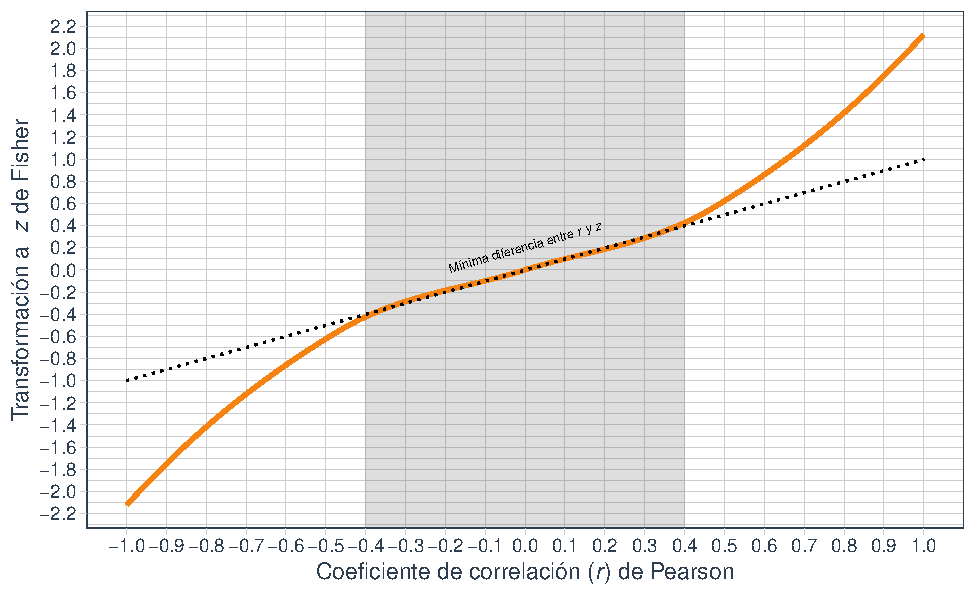
\includegraphics{Meta-analysis_files/figure-latex/rvsz-1.pdf}
\caption{\label{fig:rvsz}Asociación entre coeficientes de correlación \emph{r} de Pearson (eje \emph{X}), y su transformación a \emph{z} de Fisher (eje \emph{Y}). La línea naranja representa la asociación entre valores \emph{r} y \emph{z}; como referencia, la línea negra punteada representa igualdad entre ejes (\emph{y} = \emph{x}). Como se puede ver, cuando \emph{r} está aproximadamente entre -0.4 y 0.4 (rectángulo gris), los valores \emph{r} y \emph{z} son casi idénticos. Para valores más extremos, el valor de \emph{z} se aleja progresivamente del valor de \emph{r}.}
\end{figure}

Por supuesto, si decides reportar los resultados de tu meta-análisis en coeficientes \emph{r} de Pearson, siempre puedes hacer lo mismo con el error estándar y los límites del intervalo de confianza del 95\% (todos valores en \emph{z} de Fisher, pues fue el tamaño de efecto que meta-analizamos).

\hypertarget{heterog-inf}{%
\subsection{Más información sobre heterogeneidad}\label{heterog-inf}}

Es importante tener en cuenta que la heterogeneidad no es un \emph{supuesto} que se deba cumplir al hacer un meta-análisis, y por ende una heterogeneidad moderada o alta no invalida sus resultados. Sencillamente es información útil que se debe reportar y tener en cuenta al interpretar el resultado de un meta-análisis. En este caso, la presencia de heterogeneidad sugiere que los estudios meta-analizados varían y no suelen reportar resultados similares.

De manera general, y para decirlo de manera más técnica, la presencia de heterogeneidad estadística es indicativa de una variación entre los estudios en la magnitud y la dirección de la estimación del efecto estudiado (para más información y ejemplos, ver \protect\hyperlink{ref-sedgwickMetaanalysesWhatHeterogeneity2015}{Sedgwick, 2015}).

Por esto, reportar información detallada acerca de la heterogeneidad de los estudios meta-analizados es siempre útil. De hecho, además de reportar los estadísticos \(\tau^2\), \(\tau\), \(I^2\) y \(Q\) (como expliqué en la sección \ref{meta-interp}), podemos fácilmente calcular los intervalos de confianza para \(\tau^2\), \(\tau\), e \(I^2\) (además de \(H^2\), que no he usado) con la función \texttt{confint}.

\begin{Shaded}
\begin{Highlighting}[]
\FunctionTok{confint}\NormalTok{(res)}
\end{Highlighting}
\end{Shaded}

\begin{ROut}{Consola de R: Output~\thetcbcounter}
                \begin{footnotesize}
                \begin{verbatim} 
       estimate   ci.lb   ci.ub 
tau^2    0.0081  0.0017  0.0378 
tau      0.0901  0.0412  0.1944 
I^2(%)  61.7324 25.2799 88.2545 
H^2      2.6132  1.3383  8.5139 
 \end{verbatim}
                \end{footnotesize}
                \end{ROut}

Para \(\tau^2\), el hecho de que los límites del intervalo de confianza no crucen el 0 (es decir, no hay un límite negativo y otro positivo; en nuestro caso, ambos son positivos: IC 95\% {[}0.0017, 0.0378{]}), también sugiere que que hay heterogeneidad entre los estudios que meta-analizamos.

\hypertarget{reporte2}{%
\subsubsection{Reporte del meta-análisis con intervalos de confianza para medidas de heterogeneidad}\label{reporte2}}

Estos intervalos de confianza que también pueden ser reportados junto a sus correspondientes estadísticos. Entonces, esto se podría resumir, por ejemplo, como:

\begin{tcolorbox}[enhanced,attach boxed title to top center={yshift=-3mm,yshifttext=-1mm},
  colback=iacol!5!white,colframe=iacol!75!white,colbacktitle=iacol,
  title=Ejemplo de reporte con intervalos de confianza para heterogeneidad,fonttitle=\bfseries,
  boxed title style={size=small,colframe=iacol} ]
  
El meta-análisis incluyó 16 estudios que examinaron la relación entre la escrupulosidad y la adherencia a la medicación. Los estudios incluidos variaron en cuanto al diseño, la población de pacientes y la intervención evaluada. Los resultados del meta-análisis indicaron una asociación positiva significativa entre la escrupulosidad y la adherencia a la medicación ($z$ ± $se$ = 0.15 ± 0.032, IC 95\% [0.09, 0.21]; $Z$ = 4.75, $p$ < .0001). La heterogeneidad en torno al tamaño medio del efecto entre los estudios incluidos fue moderada pero significativa ($\tau^2$ ± $se$ =  0.0081 ± 0.0055, IC 95\% [0.0017, 0.0378]; $\tau$ = 0.0901, IC 95\% [0.0412, 0.1944]; $Q$(15) =  38.16, $p$ < .001; $I^2$ = 61.7\%, IC 95\% [25.28\%, 88.25\%]). Se observó una amplia variabilidad en el tamaño del efecto entre los estudios, lo que sugiere que los resultados deben interpretarse con precaución. A pesar de estas limitaciones, los hallazgos sugieren que es probable que la escrupulosidad tenga un efecto positivo en la adherencia a la medicación. Es importante tener en cuenta que la calidad metodológica de los estudios incluidos en el meta-análisis fue variable, lo que puede afectar la validez y generalización de las conclusiones.

\end{tcolorbox}

De nuevo, recuerda que siempre es buena idea citar tablas y figuras relevantes junto al reporte de los resultados que ilustran. Aunque aún no hemos creado ninguna figura, al reportar un meta-análisis es buena idea al menos citar (e incluir) un \emph{Forest plot} (diagrama de bosque; \ref{forest-inf}), y un \emph{Funnel plot} (diagrama de embudo; sección \ref{funnel-inf}). Más adelante explicaré cómo crear e interpretar estas figuras.

\hypertarget{diag-inf}{%
\subsection{Diagnóstico de influencia}\label{diag-inf}}

Otro aspecto importante de un meta-análisis, es determinar si alguno o algunos de los estudios meta-analizados es o son particularmente influyentes en nuestro resultado\footnote{Por ejemplo, si estuviésemos meta-analizando 20 estudios, de los cuales 19 tienen un \emph{n} de 100, pero el otro tiene un \emph{n} de 10.000, éste último tendrá una influencia enorme en nuestro resultado. Sería preocupante que nuestro meta-análisis sea dependiente principalmente de un único estudio.}. Para esto, se suele usar la técnica conocida como \emph{leave-one-out}, que se refiere al resultado del meta-análisis cuando se excluye cada estudio; al estimar cómo y cuánto cambia el resultado del modelo de meta-análisis al excluir cada estudio, podemos estimar su influencia en el resultado. Dicho de otra manera, si al excluir un estudio el resultado cambia mucho, sabemos que ese estudio tiene gran influencia en el meta-análisis y sería mejor excluirlo.

Para hacer un análisis de influencia, podemos usar la función \texttt{influence} del paquete \texttt{metafor}, cuyo resultado, en este caso, asignaré a un objeto llamado \texttt{inf.res}.

\begin{Shaded}
\begin{Highlighting}[]
\NormalTok{inf.res }\OtherTok{\textless{}{-}} \FunctionTok{influence}\NormalTok{(res)}
\end{Highlighting}
\end{Shaded}

Dado que lo asigné a un objeto (\texttt{inf.res}), para ver el resultado, debo usar como comando el nombre que le di al objeto.

\begin{Shaded}
\begin{Highlighting}[]
\NormalTok{inf.res}
\end{Highlighting}
\end{Shaded}

\begin{ROut}{Consola de R: Output~\thetcbcounter}
                \begin{footnotesize}
                \begin{verbatim} 
   rstudent  dffits cook.d  cov.r tau2.del  QE.del    hat  weight    dfbs inf 
1    0.2918  0.0485 0.0025 1.1331   0.0091 37.7109 0.0568  5.6776  0.0481     
2    0.1196 -0.0031 0.0000 1.2595   0.0100 36.7672 0.1054 10.5396 -0.0032     
3    1.2740  0.2595 0.0660 0.9942   0.0075 35.3930 0.0364  3.6432  0.2623     
4    1.4711  0.3946 0.1439 0.9544   0.0068 33.5886 0.0562  5.6195  0.3994     
5    0.8622  0.1838 0.0339 1.0505   0.0082 36.5396 0.0441  4.4069  0.1837     
6   -0.9795 -0.2121 0.0455 1.0639   0.0084 37.1703 0.0411  4.1094 -0.2112     
7    0.2177  0.0296 0.0010 1.1740   0.0094 37.6797 0.0714  7.1362  0.0296     
8   -0.9774 -0.3120 0.1001 1.1215   0.0084 36.1484 0.0889  8.8886 -0.3128     
9    0.7264  0.1392 0.0195 1.0561   0.0083 37.0495 0.0379  3.7886  0.1387     
10  -1.8667 -0.5861 0.2198 0.8502   0.0047 25.0661 0.1058 10.5826 -0.5430     
11  -1.4985 -0.2771 0.0756 1.0073   0.0077 35.6617 0.0369  3.6922 -0.2791     
12   1.8776  0.4918 0.2148 0.8819   0.0059 31.9021 0.0511  5.1150  0.5059     
13  -1.1892 -0.2939 0.0859 1.0550   0.0080 36.3291 0.0587  5.8732 -0.2941     
14  -0.0020 -0.0423 0.0021 1.2524   0.0100 37.7339 0.0998  9.9778 -0.0434     
15   0.8066  0.2126 0.0459 1.0907   0.0083 35.8385 0.0684  6.8403  0.2125     
16  -0.7160 -0.1656 0.0280 1.0853   0.0087 37.7017 0.0411  4.1094 -0.1642     
 \end{verbatim}
                \end{footnotesize}
                \end{ROut}

Esto me muestra gran cantidad de datos de cada estudio (en este caso, lo presento como una tabla sin formato, tal cual se ve en la consola de R), y contiene información que puede parecer muy compleja; sin embargo, como verás, la última columna resume la interpretación general de estos resultados de influencia, facilitando muchísimo su interpretación.

Las columnas que incluye son:

\begin{itemize}
\item
  \texttt{rstudent}: residuos estandarizados externamente. Esto \textbf{no} corresponde al coeficiente de correlación de cada estudio, sino a la diferencia entre el tamaño de efecto observado en cada estudio, y la predicción de dicho valor cuando dicho estudio se elimina del meta-análisis
\item
  \texttt{dffits}: diferencia de ajuste(s) (en inglés \emph{difference in fit(s)}). Es una medida diagnóstica de la influencia de cada punto en una regresión (en este caso, cada estudio en un meta-análisis) propuesta originalmente por Belsley et al. (\protect\hyperlink{ref-belsleyRegressionDiagnosticsIdentifying1980}{1980})
\item
  \texttt{cook.d}: Distancia de Cook (en inglés, \emph{Cook's distance}). Es otra medida diagnóstica de la influencia, propuesta originalmente por Cook (\protect\hyperlink{ref-cookDetectionInfluentialObservation1977}{1977}). Es conceptualmente idéntica a DFFITS (\texttt{dffits}), y de hecho existe una fórmula para convertir una medida en la otra (\protect\hyperlink{ref-Henry2003}{Henry et al., 2003}). Aunque no hay un acuerdo absoluto al respecto, comúnmente se asume que valores mayores a 1 (\(D_{i} > 1\)), representan puntos (o, en este caso, estudios) influyentes en un modelo (\protect\hyperlink{ref-cookResidualsInfluenceRegression1982}{Cook \& Weisberg, 1982}), que probablemente deban ser excluidos
\item
  \texttt{cov.r}: relación (o proporción) de covarianza. Es el determinante de la matriz de varianza-covarianza de las estimaciones de los parámetros basadas en el conjunto de datos, cuando cada estudio se elimina del meta-análisis, dividido por el mismo determinante de la matriz de varianza-covarianza cuando se incluyen todos los estudios. Sé que suena complejo, pero básicamente, un valor menor a 1 indica que la eliminación de ese estudio produce estimaciones más precisas de los coeficientes del modelo
\item
  \texttt{tau2.del}: es la heterogeneidad (residual) \(\tau^2\) cuando se elimina cada estudio
\item
  \texttt{QE.del}: similar al resultado anterior, este se refiere al estadístico \(Q\) obtenido cuando se excluye cada estudio
\item
  \texttt{hat}: los valores \emph{hat} (\(h\)) son una medida estandarizada de la distancia de cada punto a la media de la variable predictora. Mientras valores cercanos a 0 indican que no hay un valor preocupante, valores cercanos a 1, aunque no indican directamente alta influencia de algún punto, ciertamente nos indican que vale la pena investigar más. Los valores \emph{hat} están abiertos a la interpretación, pero un valor de corte que es común es el doble de la media de los todos valores \emph{hat} (\(\overline{h}\)); cualquier estudio con un valor mayor debe ser examinado con cuidado
\item
  \texttt{weight}: peso asignado a cada estudio
\item
  \texttt{dfbs}: el valor de \texttt{dfbs} (o \emph{DFBETAS}) indica cuántas desviaciones estándar cambia el coeficiente estimado después de excluir cada estudio del modelo de meta-análisis
\item
  \texttt{inf}: por suerte, esta columna \texttt{inf} resume esta información por nosotros. Cualquier estudio que se considere influyente, teniendo en cuenta la diferencia de ajuste, la distancia de Cook, los valores \emph{hat} o \emph{DFBETAS}, será señalado acá como influyente, usando asteriscos
\end{itemize}

Aunque hay mucha información, lo más importante ahora es mirar la última columna, llamada \texttt{inf}. Si ahí aparecieran asteriscos para algún estudio meta-analizado (que no es nuestro caso), sugeriría que ese estudio es particularmente influyente y podría ser necesario eliminarlo del meta-análisis.

Por último, podemos también ver ésta información que tenemos guardada en el objeto \texttt{inf.res}, de manera gráfica, usando la función \texttt{plot} (Fig. \ref{fig:infplot}).

\begin{Shaded}
\begin{Highlighting}[]
\FunctionTok{plot}\NormalTok{(inf.res)}
\end{Highlighting}
\end{Shaded}

\begin{figure}
\centering
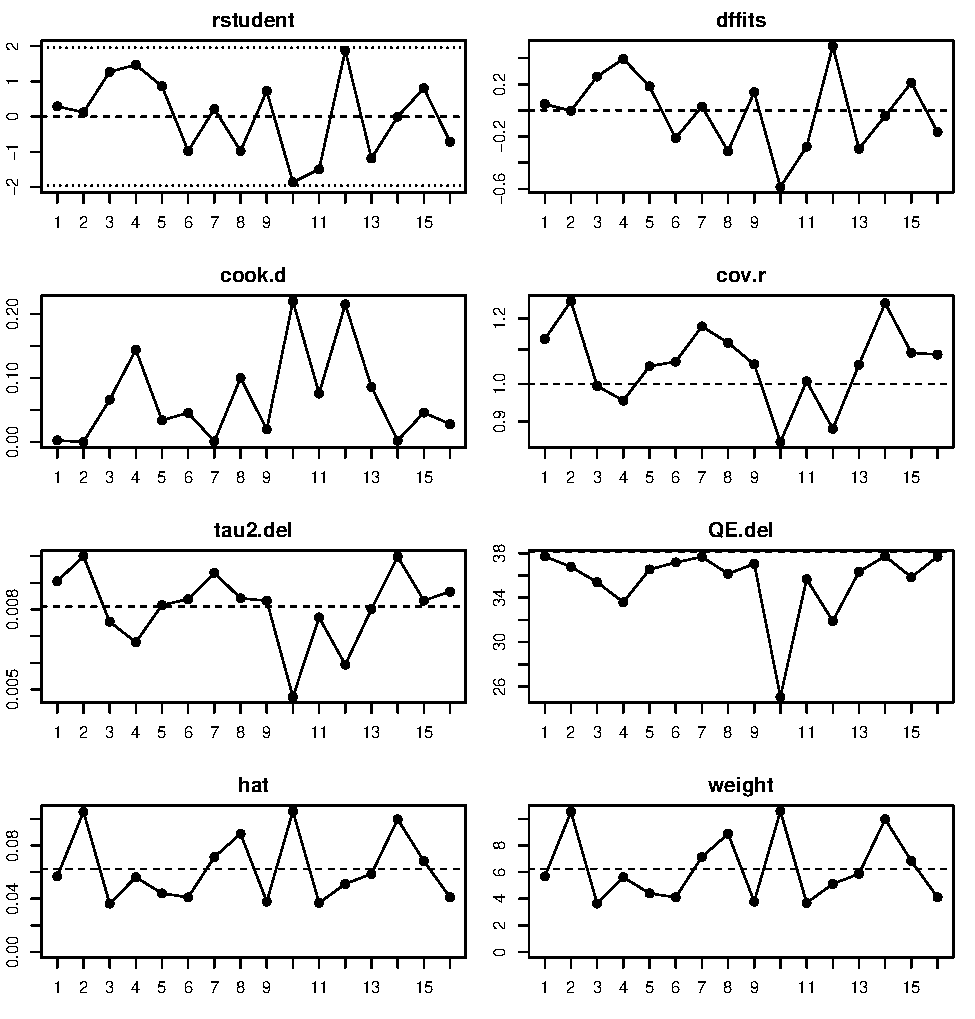
\includegraphics{Meta-analysis_files/figure-latex/infplot-1.pdf}
\caption{\label{fig:infplot}Diagnóstico de influencia. Estudios particularmente influyentes serían representados con un punto rojo. Los números 1 a 16 en el eje \emph{X} representan cada estudio, como lo definimos en columna \texttt{study\_id} de la Tabla \ref{tab:estructuramod}. En este caso, no hay ningún estudio que se considere demasiado influyente, por lo éste análisis sugiere que no es necesario excluir ningún estudio de nuestro meta-análisis.}
\end{figure}

Más adelante, en la sección \ref{todas-combinaciones}, daré más información y técnicas más completas para identificar estudios atípicos que podrían sesgar nuestra estimación del efecto \emph{real}.

\hypertarget{forest-inf}{%
\subsection{\texorpdfstring{\emph{Forest plot} (diagrama de bosque)}{Forest plot (diagrama de bosque)}}\label{forest-inf}}

Hacer un diagrama de bosque (\emph{forest plot}) que resuma nuestro meta-análisis usando \href{https://www.metafor-project.org/doku.php}{\texttt{metafor}} es muy fácil; sólo tenemos que usar la función \texttt{forest}, usando como argumento el objeto al que asignamos los resultados de nuestro meta-análisis (en nuestro caso, \texttt{res}).

\begin{Shaded}
\begin{Highlighting}[]
\FunctionTok{forest}\NormalTok{(res)}
\end{Highlighting}
\end{Shaded}

Esto produce la Figura \ref{fig:for-plot1}.

\begin{figure}
\centering
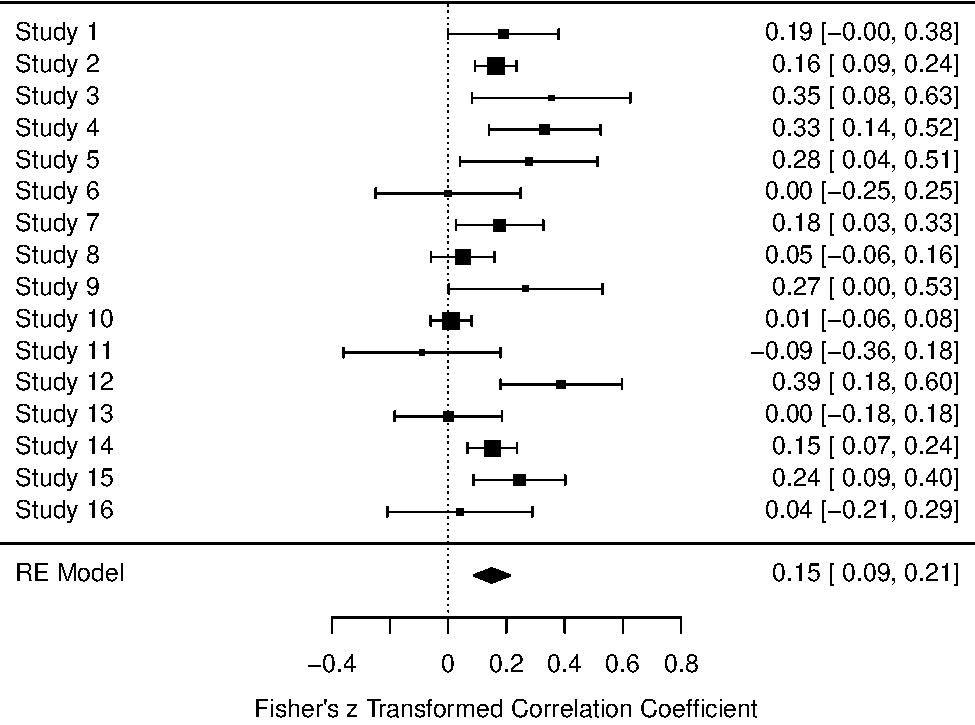
\includegraphics{Meta-analysis_files/figure-latex/for-plot1-1.pdf}
\caption{\label{fig:for-plot1}\emph{Forest plot} básico de \href{https://www.metafor-project.org/doku.php}{metafor}. Para cada estudio meta-analizado, tenemos el efecto (correlación, en este caso en valores \emph{z} de Fisher), así como sus intervalos de confianza entre paréntesis cuadrados. Esta misma información está representada gráficamente, con los cuadrados representando el efecto de cada estudio así como sus intervalos de confianza como barras de error, y el tamaño de muestra representado por el tamaño del cuadrado. Bajo estos resultados, tenemos nuestro meta-análisis, con el mismo formato en texto, pero representando el efecto y sus intervalos de confianza con un diamante.}
\end{figure}

Como se puede ver en las Figuras \ref{fig:for-plot1}, \ref{fig:for-plot2} y \ref{fig:for-plot3b} (que son versiones del mismo \emph{forest plot}), no es una sorpresa que el análisis nos sugiera bastante heterogeneidad; las correlaciones encontradas entre los diferentes estudios varían mucho (están entre -0.09 y 0.37), y aunque son positivas en la mayoría de los casos, en algunos son prácticamente 0 o incluso negativas.

Para una versión más completa y anotada, también usando el \emph{plot} básico de \href{https://www.metafor-project.org/doku.php}{\texttt{metafor}}, pero agregando encabezados de cada columna en español, nombres de los estudios meta-analizados\footnote{En este caso, dado que tenemos los autores y los años de publicación de cada estudio en columnas separadas, pegué las columnas \texttt{authors} y \texttt{year} separadas por una coma y un espacio: \texttt{paste(dat\$authors,\ dat\$year,\ sep\ =\ ",\ ")} como argumento \texttt{slab}.} así como una columna con los pesos dados a cada estudio, y detalles del modelo final\footnote{Estas opciones están explicadas \href{https://search.r-project.org/CRAN/refmans/metafor/html/forest.rma.html}{acá}.}, podemos hacer algo como esto:

\begin{Shaded}
\begin{Highlighting}[]
\CommentTok{\# forest plot con anotaciones adicionales}
\FunctionTok{forest}\NormalTok{(res, }\AttributeTok{cex =} \FloatTok{0.75}\NormalTok{, }\AttributeTok{xlim =} \FunctionTok{c}\NormalTok{(}\SpecialCharTok{{-}}\FloatTok{1.6}\NormalTok{, }\FloatTok{1.6}\NormalTok{),}
       \AttributeTok{slab =} \FunctionTok{paste}\NormalTok{(dat}\SpecialCharTok{$}\NormalTok{authors, dat}\SpecialCharTok{$}\NormalTok{year, }\AttributeTok{sep =} \StringTok{", "}\NormalTok{),}
       \AttributeTok{showweights =} \ConstantTok{TRUE}\NormalTok{,}
       \AttributeTok{xlab =} \StringTok{"Coeficiente de correlación (z de Fisher)"}\NormalTok{,}
       \AttributeTok{digits =} \FunctionTok{c}\NormalTok{(}\DecValTok{2}\NormalTok{,3L),}
       \AttributeTok{mlab =} \FunctionTok{bquote}\NormalTok{(}\FunctionTok{paste}\NormalTok{(}\StringTok{"Modelo EA: Q("}\NormalTok{, .(res}\SpecialCharTok{$}\NormalTok{k }\SpecialCharTok{{-}}\NormalTok{ res}\SpecialCharTok{$}\NormalTok{p), }\StringTok{") = "}\NormalTok{,}
\NormalTok{     .(}\FunctionTok{formatC}\NormalTok{(res}\SpecialCharTok{$}\NormalTok{QE, }\AttributeTok{digits =} \DecValTok{2}\NormalTok{, }\AttributeTok{format =} \StringTok{"f"}\NormalTok{)),}
     \StringTok{", p "}\NormalTok{, .(scales}\SpecialCharTok{::}\FunctionTok{pvalue}\NormalTok{(res}\SpecialCharTok{$}\NormalTok{pval)), }\StringTok{"; "}\NormalTok{, I}\SpecialCharTok{\^{}}\DecValTok{2}\NormalTok{, }\StringTok{" = "}\NormalTok{,}
\NormalTok{     .(}\FunctionTok{formatC}\NormalTok{(res}\SpecialCharTok{$}\NormalTok{I2, }\AttributeTok{digits =} \DecValTok{1}\NormalTok{, }\AttributeTok{format =} \StringTok{"f"}\NormalTok{)), }\StringTok{"\%"}\NormalTok{)))}
\CommentTok{\# agregar encabezados a las columnas (valores de X y Y deben ser ajustados)}
\NormalTok{op }\OtherTok{\textless{}{-}} \FunctionTok{par}\NormalTok{(}\AttributeTok{cex =} \FloatTok{0.8}\NormalTok{, }\AttributeTok{font =} \DecValTok{2}\NormalTok{) }
\FunctionTok{text}\NormalTok{(}\AttributeTok{x =} \SpecialCharTok{{-}}\FloatTok{1.6}\NormalTok{, }\AttributeTok{y =} \DecValTok{18}\NormalTok{, }\AttributeTok{labels =} \StringTok{"Autor(es), Año"}\NormalTok{, }\AttributeTok{pos =} \DecValTok{4}\NormalTok{)}
\FunctionTok{text}\NormalTok{(}\AttributeTok{x =} \DecValTok{0}\NormalTok{, }\AttributeTok{y =} \DecValTok{18}\NormalTok{, }\AttributeTok{labels =} \StringTok{"Efecto e IC"}\NormalTok{, }\AttributeTok{pos =} \DecValTok{4}\NormalTok{)}
\FunctionTok{text}\NormalTok{(}\AttributeTok{x =} \DecValTok{1}\NormalTok{, }\AttributeTok{y =} \DecValTok{18}\NormalTok{, }\AttributeTok{labels =} \StringTok{"Peso"}\NormalTok{, }\AttributeTok{pos =} \DecValTok{2}\NormalTok{)}
\FunctionTok{text}\NormalTok{(}\AttributeTok{x =} \FloatTok{1.6}\NormalTok{, }\AttributeTok{y =} \DecValTok{18}\NormalTok{, }\AttributeTok{labels =} \StringTok{"Corr. [95\% IC]"}\NormalTok{, }\AttributeTok{pos =} \DecValTok{2}\NormalTok{)}
\end{Highlighting}
\end{Shaded}

\begin{figure}
\centering
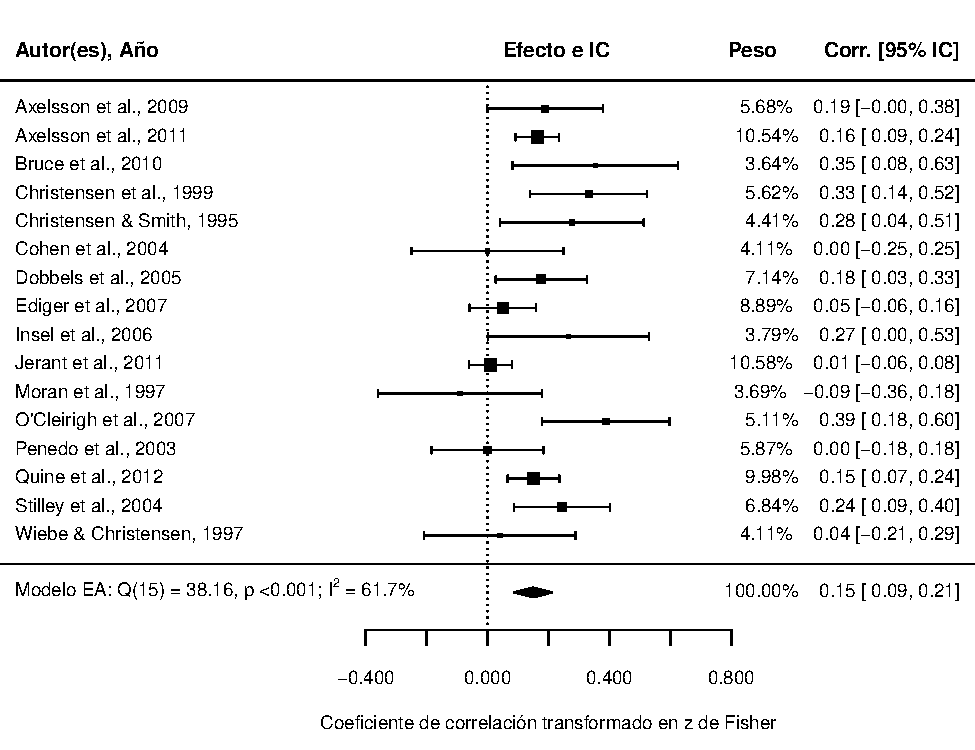
\includegraphics{Meta-analysis_files/figure-latex/for-plot2-1.pdf}
\caption{\label{fig:for-plot2}\emph{Forest plot} anotado, creado con \href{https://www.metafor-project.org/doku.php}{metafor}. En esta versión agregué algunos encabezados en español, así como estadísticos generales del modelo de meta-análisis. Modelo EA se refiere al modelo meta-analizado, de efectos aleatorios.}
\end{figure}

O, para un \emph{forest plot} quizás más sofisticado, se puede usar la función \href{https://cran.r-project.org/web/packages/metaviz/vignettes/metaviz.html\#creating-forest-plots-with-function-viz_forest}{\texttt{viz\_forest}} del paquete \href{https://cran.r-project.org/web/packages/metaviz/vignettes/metaviz.html}{\texttt{metaviz}}, en alguna de sus variantes y colores.

\begin{Shaded}
\begin{Highlighting}[]
\CommentTok{\# A. Variante "classic" (no tiene que ser definida, pues es la opción por defecto)}
\FunctionTok{viz\_forest}\NormalTok{(res, }
           \AttributeTok{study\_labels =} \FunctionTok{paste}\NormalTok{(dat}\SpecialCharTok{$}\NormalTok{authors, dat}\SpecialCharTok{$}\NormalTok{year, }\AttributeTok{sep =} \StringTok{", "}\NormalTok{),}
           \AttributeTok{xlab =} \StringTok{"Correlación"}\NormalTok{, }
           \AttributeTok{annotate\_CI =} \ConstantTok{TRUE}\NormalTok{,}
           \AttributeTok{summary\_label =} \StringTok{"Resumen"}\NormalTok{,}
           \AttributeTok{text\_size =} \FloatTok{2.6}\NormalTok{,}
           \AttributeTok{x\_trans\_function =}\NormalTok{ tanh)}

\CommentTok{\# B. Variante "thick"}
\FunctionTok{viz\_forest}\NormalTok{(res, }
           \AttributeTok{study\_labels =} \FunctionTok{paste}\NormalTok{(dat}\SpecialCharTok{$}\NormalTok{authors, dat}\SpecialCharTok{$}\NormalTok{year, }\AttributeTok{sep =} \StringTok{", "}\NormalTok{),}
           \AttributeTok{xlab =} \StringTok{"Correlación"}\NormalTok{, }
           \AttributeTok{variant =} \StringTok{"thick"}\NormalTok{,}
           \AttributeTok{col =} \StringTok{"Greens"}\NormalTok{,}
           \AttributeTok{annotate\_CI =} \ConstantTok{TRUE}\NormalTok{,}
           \AttributeTok{summary\_label =} \StringTok{"Resumen"}\NormalTok{,}
           \AttributeTok{text\_size =} \FloatTok{2.6}\NormalTok{,}
           \AttributeTok{x\_trans\_function =}\NormalTok{ tanh)}

\CommentTok{\# C. Variante "rain"}
\FunctionTok{viz\_forest}\NormalTok{(res, }
           \AttributeTok{study\_labels =} \FunctionTok{paste}\NormalTok{(dat}\SpecialCharTok{$}\NormalTok{authors, dat}\SpecialCharTok{$}\NormalTok{year, }\AttributeTok{sep =} \StringTok{", "}\NormalTok{),}
           \AttributeTok{xlab =} \StringTok{"Correlación"}\NormalTok{, }
           \AttributeTok{variant =} \StringTok{"rain"}\NormalTok{,}
           \AttributeTok{col =} \StringTok{"Oranges"}\NormalTok{,}
           \AttributeTok{annotate\_CI =} \ConstantTok{TRUE}\NormalTok{,}
           \AttributeTok{summary\_label =} \StringTok{"Resumen"}\NormalTok{,}
           \AttributeTok{text\_size =} \FloatTok{2.6}\NormalTok{,}
           \AttributeTok{x\_trans\_function =}\NormalTok{ tanh)}
\end{Highlighting}
\end{Shaded}

Con el código anterior genero las siguientes tres versiones del mismo \emph{forest plot} (Fig. \ref{fig:for-plot3b}) usando diferentes variantes y escalas de colores, y transformando de vuelta los coeficientes de \emph{z} de Fisher a \emph{r} de Pearson (con el argumento \texttt{x\_trans\_function\ =\ tanh}). Por supuesto, es cuestión de gusto cuál usar.

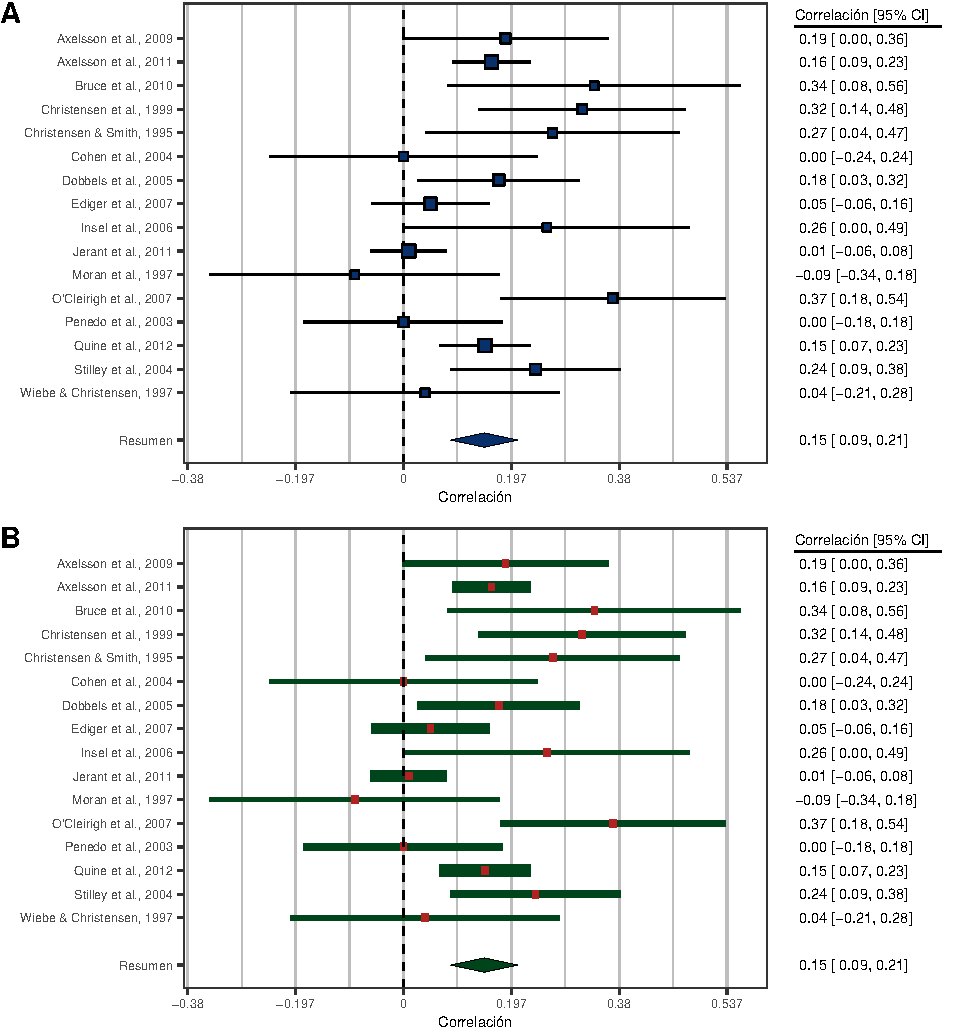
\includegraphics{Meta-analysis_files/figure-latex/for-plot3-1.pdf}

\begin{figure}
\centering
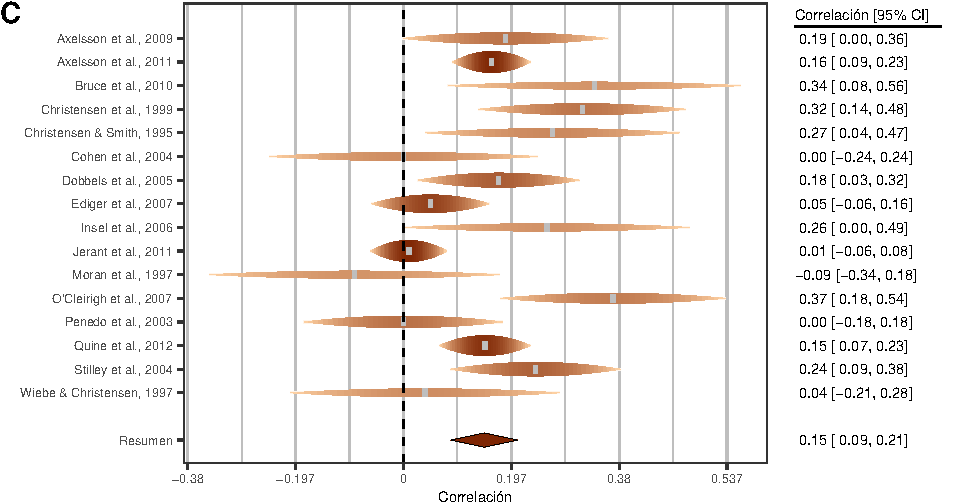
\includegraphics{Meta-analysis_files/figure-latex/for-plot3b-1.pdf}
\caption{\label{fig:for-plot3b}Variantes de \emph{forest plots} creados con \href{https://cran.r-project.org/web/packages/metaviz/vignettes/metaviz.html}{metaviz}. \textbf{A.} Variante clásica (opción por defecto). \textbf{B.} Variante ``thick'' y escala de colores ``Greens''. \textbf{C.} Variante ``rain'' y escala de colores ``Oranges''.}
\end{figure}

\hypertarget{funnel-inf}{%
\subsection{\texorpdfstring{\emph{Funnel plot} (diagrama de embudo), regresión de Egger y sesgo de estudios pequeños}{Funnel plot (diagrama de embudo), regresión de Egger y sesgo de estudios pequeños}}\label{funnel-inf}}

La creación e interpretación del \emph{Funnel plot} es crucial, y aporta información muy importante acerca de un meta-análisis. Sin embargo, es en donde más errores se cometen.

\hypertarget{err-funnel-egger}{%
\subsubsection{\texorpdfstring{Errores en la interpretación del \emph{Funnel plot} y la regresión de Egger}{Errores en la interpretación del Funnel plot y la regresión de Egger}}\label{err-funnel-egger}}

El principal error que la mayoría de los investigadores podemos cometer\footnote{Me incluyo pues por supuesto también soy culpable de haber cometido este error en el pasado, incluyendo algunas ideas que expuse en mi video sobre meta-análisis en \emph{jamovi} (\protect\hyperlink{ref-leongomezMetaanalysis2021}{Leongómez, 2021}).}, es concluir que un meta-análisis tiene (o no) riesgo de sufrir de sesgos de publicación, simplemente basándonos en la evaluación de la asimetría en el \emph{funnel plot} y la regresión de Egger (\protect\hyperlink{ref-eggerBiasMetaanalysisDetected1997}{Egger et al., 1997}) (sección \ref{reg-egger}).

Estos métodos, sin embargo, no son pruebas exclusivas de sesgo de publicación, sino de sesgo de estudios de tamaño muestral pequeño (ver e.g. \protect\hyperlink{ref-schwarzerSmallStudyEffectsMetaAnalysis2015}{Schwarzer et al., 2015b}), que pueden incluir sesgo de publicación, pero no se centran exclusivamente en esto (explico algunas técnicas específicas para estimar el sesgo de publicación en la sección \ref{sesgo-pub}).

A pesar de esto, tanto la regresión de Egger como el \emph{funnel plot} son interesantes, pues es importante considerar el sesgo que podrían generar estudios con tamaño de muestra pequeño en nuestra estimación del efecto \emph{real} (o, para decirlo más técnicamente, el sesgo que podrían introducir estudios con poder estadístico bajo).

\hypertarget{funnel-plot}{%
\subsubsection{\texorpdfstring{\emph{Funnel plot}}{Funnel plot}}\label{funnel-plot}}

Para crear un \emph{funnel plot} de nuestro meta-análisis con \href{https://www.metafor-project.org/doku.php}{\texttt{metafor}} sólo tenemos que usar la función \texttt{funnel}, usando como argumento el objeto al que asignamos los resultados de nuestro meta-análisis (\texttt{res}).

\begin{Shaded}
\begin{Highlighting}[]
\FunctionTok{funnel}\NormalTok{(res)}
\end{Highlighting}
\end{Shaded}

Con esto, generamos la Figura \ref{fig:funnel-plot1}.

\begin{figure}
\centering
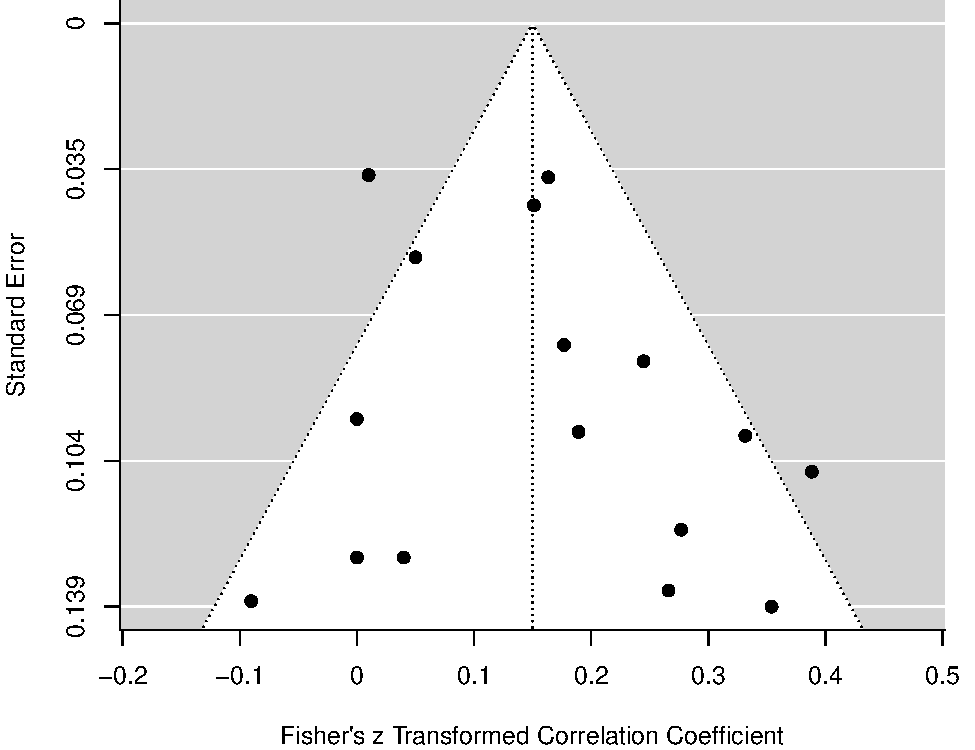
\includegraphics{Meta-analysis_files/figure-latex/funnel-plot1-1.pdf}
\caption{\label{fig:funnel-plot1}\emph{Funnel plot} básico de \href{https://www.metafor-project.org/doku.php}{metafor}. Para cada estudio meta-analizado, tenemos el efecto (correlación, en este caso en valores \emph{z} de Fisher) en el eje \emph{X}, así como su error estándar en el eje \emph{Y}. La línea punteada vertical representa el efecto \emph{real} estimado mediante nuestro meta-análisis (\emph{z} = 0.15), así que podemos ver los estudios que encontraron un efecto mayor (derecha) o menor (izquierda) que éste. A primera vista no parece haber mucha asimetría, pero es importante tener en cuenta que es un análisis muy subjetivo.}
\end{figure}

O, si queremos poner los títulos de los ejes en español, podemos hacerlo agregando los argumentos \texttt{xlab} (para el eje \(X\)) y/o \texttt{ylab} (para el eje \(Y\)), como se ve en la Figura \ref{fig:funnel-plot1a}.

\begin{Shaded}
\begin{Highlighting}[]
\FunctionTok{funnel}\NormalTok{(res, }
       \AttributeTok{xlab =} \StringTok{"Coeficiente de correlación (z de Fisher)"}\NormalTok{,}
       \AttributeTok{ylab =} \StringTok{"Error estándar"}\NormalTok{)}
\end{Highlighting}
\end{Shaded}

\begin{figure}
\centering
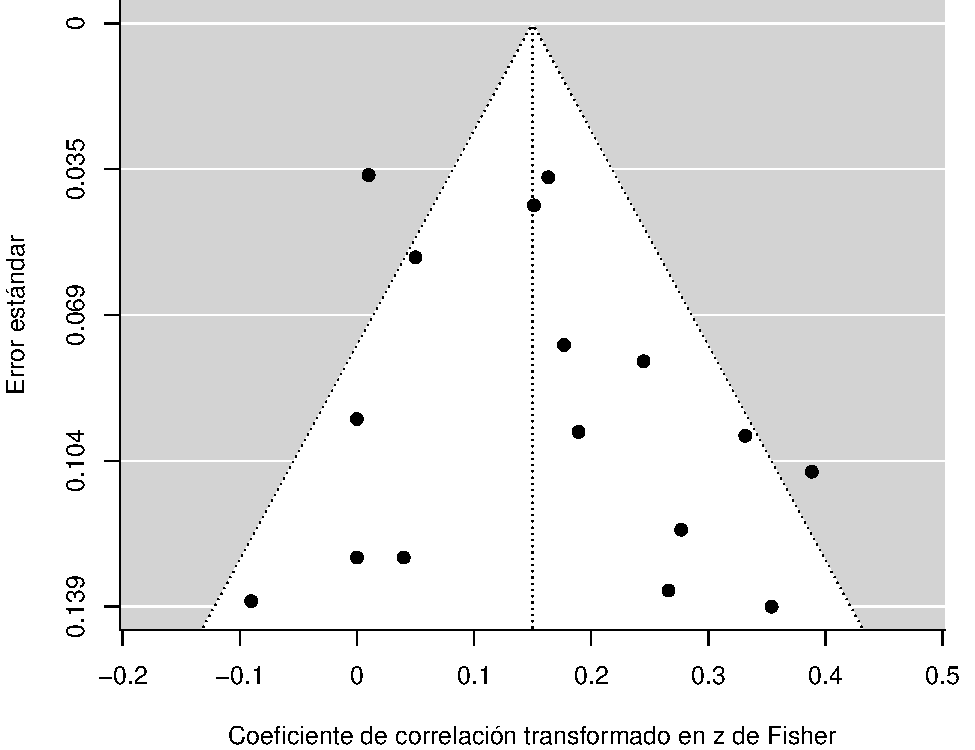
\includegraphics{Meta-analysis_files/figure-latex/funnel-plot1a-1.pdf}
\caption{\label{fig:funnel-plot1a}\emph{Funnel plot} básico de \href{https://www.metafor-project.org/doku.php}{metafor}, idéntico al de la Figura \ref{fig:funnel-plot1}, pero con títulos de ejes en español.}
\end{figure}

De nuevo, para una versión más sofisticada, se puede usar el paquete \href{https://cran.r-project.org/web/packages/metaviz/vignettes/metaviz.html}{\texttt{metaviz}}, usando la función \href{https://cran.r-project.org/web/packages/metaviz/vignettes/metaviz.html\#creating-funnel-plots-with-viz_funnel}{\texttt{viz\_funnel}}. Hay muchas opciones, pero como ejemplo, usaré la versión por defecto, agregando sólo la línea de la regresión de Egger (\texttt{egger\ =\ TRUE}; ver sección \ref{reg-egger}, más adelante), transformando los tamaños de efecto de regreso a \(r\) de Pearson (\texttt{x\_trans\_function\ =\ tanh}), y con los títulos de los ejes en español (Fig. \ref{fig:funnel-plot2}).

\begin{Shaded}
\begin{Highlighting}[]
\FunctionTok{viz\_funnel}\NormalTok{(res, }
           \AttributeTok{egger =} \ConstantTok{TRUE}\NormalTok{,}
           \AttributeTok{x\_trans\_function =}\NormalTok{ tanh,}
           \AttributeTok{ylab =} \StringTok{"Error estándar"}\NormalTok{,}
           \AttributeTok{xlab =} \StringTok{"Coeficiente de correlación"}\NormalTok{)}
\end{Highlighting}
\end{Shaded}

\begin{figure}
\centering
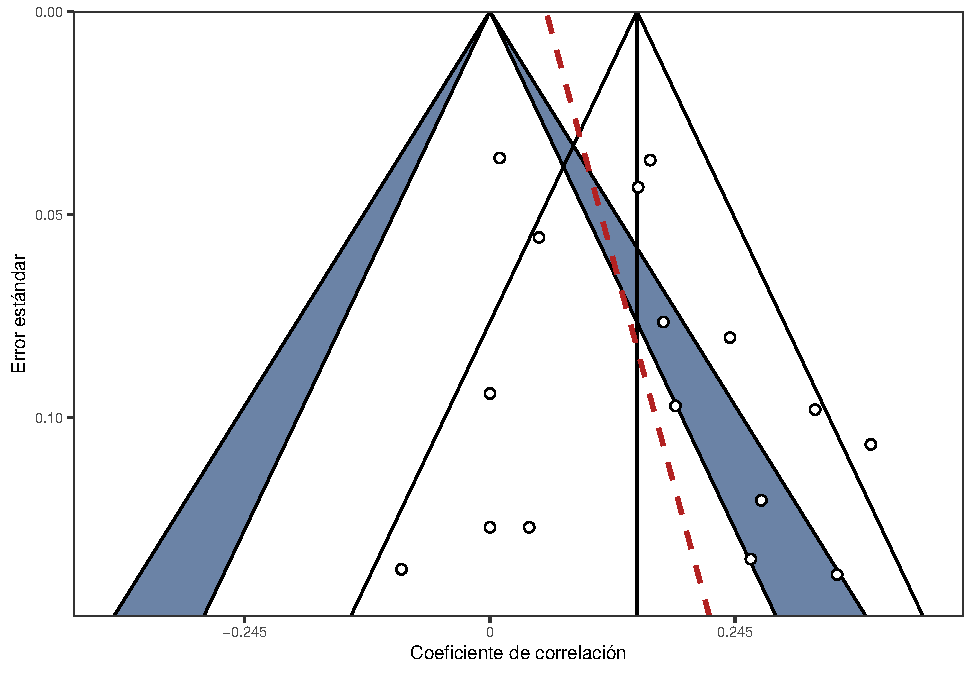
\includegraphics{Meta-analysis_files/figure-latex/funnel-plot2-1.pdf}
\caption{\label{fig:funnel-plot2}\emph{Funnel plot} creado con \href{https://cran.r-project.org/web/packages/metaviz/vignettes/metaviz.html}{metaviz}. En azul, se representa el área donde estudios, según su error (y su tamaño de muestra), tendrían un efecto significativo al 5\% (i.e.~\(p\) \textless{} 0.05), y fuera de ésta, donde tendrían un efecto significativo al 1\% (i.e.~\(p\) \textless{} 0.01). La línea negra vertical representa el efecto meta-analizado, y el triángulo a partir de su inicio, el área donde se ubican los estudios que no se diferencian significativamente del resultado del meta-análisis. La línea roja punteada, representa la regresión de Egger.}
\end{figure}

Alternativamente, el paquete \href{https://cran.r-project.org/web/packages/metaviz/vignettes/metaviz.html}{\texttt{metaviz}} tiene la función \href{https://cran.r-project.org/web/packages/metaviz/vignettes/metaviz.html\#sunset-power-enhanced-funnel-plots}{\texttt{viz\_sunset}}, que permite además mostrar el poder estadístico (o potencia) de los estudios meta-analizados para detectar un efecto de interés mediante una prueba de Wald de dos colas. De ser necesario, para entender las bases del poder estadístico, recomiendo ver \href{https://youtube.com/playlist?list\%20=\%20PLHk7UNt35ccVdyHqnQ6oXVYA6JBNFrE1x}{esta serie de videos} (\protect\hyperlink{ref-leongomezPoderRvid2020}{Leongómez, 2020b}) y/o, para mayor profundidad, leer \href{https://doi.org/10.5281/zenodo.3988776}{esta guía} (\protect\hyperlink{ref-leongomezAnalisisPoderEstadistico2020}{Leongómez, 2020a}) que publiqué anteriormente.

A continuación, muestro dos versiones de \emph{funnel plots} creados con la función \texttt{viz\_sunset} (Fig. \ref{fig:funnel-plot3}). En ambos casos, agregué el efecto \emph{real} estimado a partir del meta-análisis (\texttt{contours\ =\ TRUE}), y transformé los tamaños de efecto de regreso a \(r\) de Pearson (\texttt{x\_trans\_function\ =\ tanh}).

\begin{Shaded}
\begin{Highlighting}[]
\CommentTok{\# A. Escala de poder discreta}
\FunctionTok{viz\_sunset}\NormalTok{(res,}
           \AttributeTok{contours =} \ConstantTok{TRUE}\NormalTok{,}
           \AttributeTok{x\_trans\_function =}\NormalTok{ tanh)}

\CommentTok{\# B. Escala de poder contínua}
\FunctionTok{viz\_sunset}\NormalTok{(res, }
           \AttributeTok{contours =} \ConstantTok{TRUE}\NormalTok{,}
           \AttributeTok{x\_trans\_function =}\NormalTok{ tanh, }
           \AttributeTok{power\_contours =} \StringTok{"continuous"}\NormalTok{)}
\end{Highlighting}
\end{Shaded}

\begin{figure}
\centering
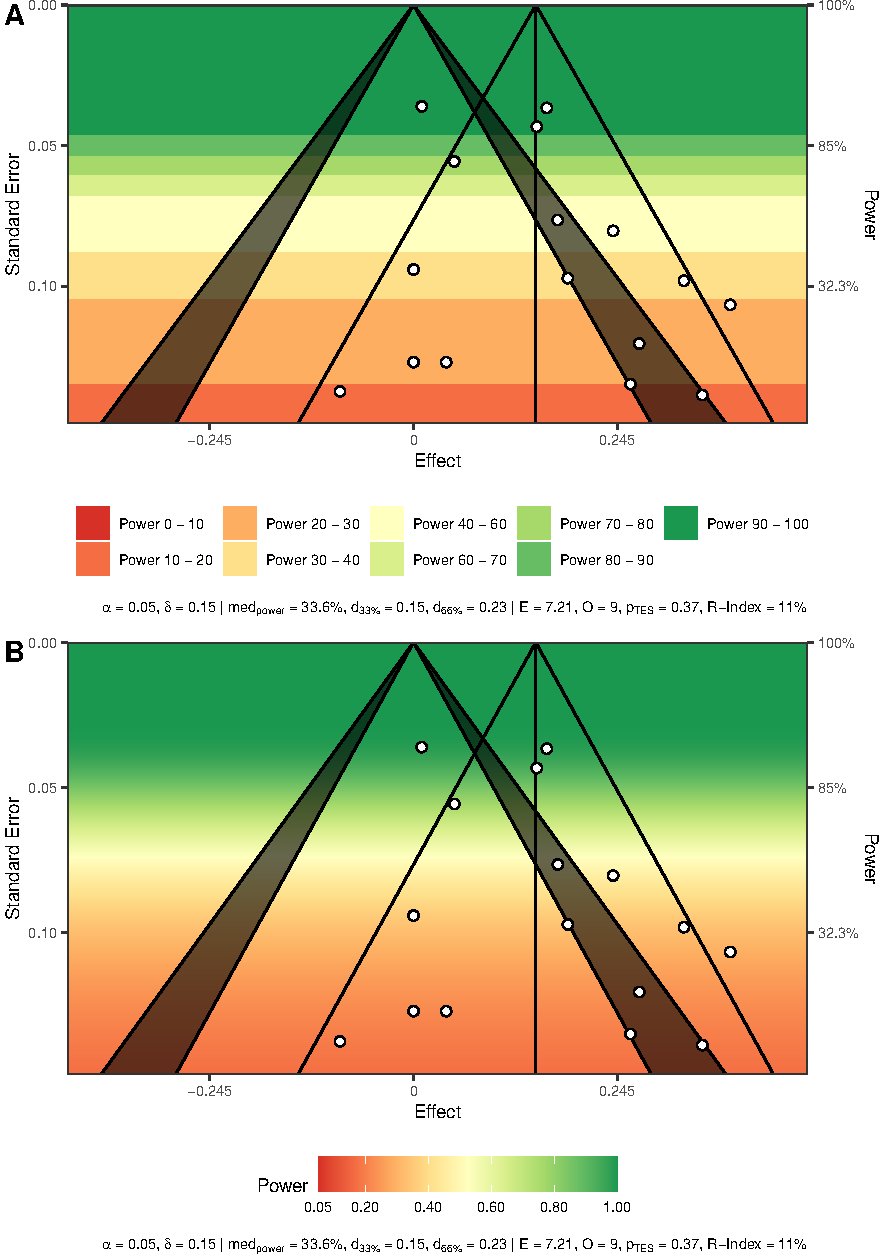
\includegraphics{Meta-analysis_files/figure-latex/funnel-plot3-1.pdf}
\caption{\label{fig:funnel-plot3}Dos versiones de \emph{funnel plot} creados con \href{https://cran.r-project.org/web/packages/metaviz/vignettes/metaviz.html}{metaviz}, usando la función viz-sunset, que estima el poder de cada estudio para detectar un efecto de interés. \textbf{A.} Poder representado por bandas dicretas de color. \textbf{B.} Poder representado de manera contínua en una escala de color. En ambos casos, y tal como en la Figura \ref{fig:funnel-plot2}, el efecto real está representado como una línea vertical, y el triángulo a partir de su inicio representa el área donde se ubican los estudios que no se diferencian significativamente del resultado del meta-análisis.}
\end{figure}

\hypertarget{reg-egger}{%
\subsubsection{Regresión de Egger}\label{reg-egger}}

Para hacer una prueba formal de sesgo de estudios pequeños (\protect\hyperlink{ref-schwarzerSmallStudyEffectsMetaAnalysis2015}{Schwarzer et al., 2015b}; \protect\hyperlink{ref-sternePublicationRelatedBias2000}{Sterne et al., 2000}, \protect\hyperlink{ref-sterneRecommendationsExaminingInterpreting2011}{2011}), a partir de la asimetría en el \emph{funnel plot}, podemos hacer una prueba o regresión de Egger (\protect\hyperlink{ref-eggerBiasMetaanalysisDetected1997}{Egger et al., 1997}).

Es importante tener en cuenta que la regresión de Egger puede carecer de poder para detectar sesgos cuando el número de estudios es pequeño; Sterne et al. (\protect\hyperlink{ref-sterneRecommendationsExaminingInterpreting2011}{2011}), de hecho, recomiendan no usar este técnica cuando tenemos menos de 10 estudios (\(k < 10\)). En nuestro ejemplo, dado que tenemos 16 estudios (\(k = 16\)), esto no debería ser un problema.

En \href{https://www.metafor-project.org/doku.php}{\texttt{metafor}}, podemos hacer una regresión de Egger con la función \texttt{regtest}, de nuevo usando como único argumento el objeto al que asignamos el resultado de nuestro meta-análisis (\texttt{res}).

\begin{Shaded}
\begin{Highlighting}[]
\FunctionTok{regtest}\NormalTok{(res)}
\end{Highlighting}
\end{Shaded}

Como se puede ver, en este caso la prueba de Egger no muestra un resultado significativo (\texttt{Test\ for\ Funnel\ Plot\ Asymmetry:\ z\ =\ 1.0216,\ p\ =\ 0.3070}), lo que sugiere que no hay sesgo de estudios pequeños.

\begin{ROut}{Consola de R: Output~\thetcbcounter}
                \begin{footnotesize}
                \begin{verbatim} 
Regression Test for Funnel Plot Asymmetry

Model:     mixed-effects meta-regression model
Predictor: standard error

Test for Funnel Plot Asymmetry: z = 1.0216, p = 0.3070
Limit Estimate (as sei -> 0):   b = 0.0790 (CI: -0.0686, 0.2266)
 \end{verbatim}
                \end{footnotesize}
                \end{ROut}

Con base en esto, y la inspección visual subjetiva del \emph{funnel plot}, muchos investigadores podrían concluir, sin sustento adecuado, que en el meta-análisis no hay sesgo de publicación. Sin embargo, como mencioné antes (sección \ref{err-funnel-egger}), estas pruebas no se centran en el sesgo de publicación sino en el sesgo de estudios pequeños. En otras palabras, con base en esto, lo único que podemos concluir correctamente, es que no hay sesgo de estudios pequeños (en la sección \ref{sesgo-pub} a continuación, explicaré cómo evaluar si hay sesgo de publicación).

\hypertarget{sesgo-pub}{%
\subsection{\texorpdfstring{Sesgo de publicación (\emph{publication bias})}{Sesgo de publicación (publication bias)}}\label{sesgo-pub}}

Existen diferentes opciones para estimar el sesgo de publicación de un meta-análisis. En esta sección, me centraré en dos: el método de recorte y relleno (\emph{trim and fill}; sección \ref{trim-fill}), y el modelo de función de peso de Vevea y Hedges (sección \ref{vevea-hedges}), que es uno de los modelos de selección más conocidos para evaluar sesgos de publicación.

\hypertarget{trim-fill}{%
\subsubsection{\texorpdfstring{Método \emph{trim and fill} (recorte y relleno)}{Método trim and fill (recorte y relleno)}}\label{trim-fill}}

El método de recorte y relleno (\emph{trim and fill}) es una técnica no paramétrica para aumentar datos (\protect\hyperlink{ref-duvalNonparametricTrimFill2000}{Duval \& Tweedie, 2000a}, \protect\hyperlink{ref-duvalTrimFillSimple2000}{2000b}; ver también \protect\hyperlink{ref-duvalTrimFillMethod2005}{Duval, 2005}). Este método estima los estudios potencialmente ausentes debido al sesgo de publicación en el gráfico de embudo, y ajusta la estimación del efecto \emph{real}. Aunque muy útil, es importante tener en cuenta que este método tiene algunas limitaciones:

\begin{itemize}
\item
  No debe entenderse como una forma de obtener una estimación más ``válida'' del efecto \emph{real}, sino como una forma de examinar qué tan sensibles son los resultados a una forma particular de sesgo de publicación
\item
  No se puede usar en modelos con moderadores, como los que explico en la sección \ref{met-moderation}
\end{itemize}

En \href{https://www.metafor-project.org/doku.php}{\texttt{metafor}}, el método de recorte y relleno (\emph{trim and fill}) se hace simplemente con la función \texttt{trimfill}, de nuevo usando como argumento el objeto al que asignamos el resultado de nuestro meta-análisis (\texttt{res}). En este caso, asignaré el resultado de esta función a un objeto que llamaré \texttt{tf}.

\begin{Shaded}
\begin{Highlighting}[]
\NormalTok{tf }\OtherTok{\textless{}{-}} \FunctionTok{trimfill}\NormalTok{(res)}
\NormalTok{tf}
\end{Highlighting}
\end{Shaded}

\begin{ROut}{Consola de R: Output~\thetcbcounter}
                \begin{footnotesize}
                \begin{verbatim} 
Estimated number of missing studies on the left side: 2 (SE = 2.7118)

Random-Effects Model (k = 18; tau^2 estimator: REML)

tau^2 (estimated amount of total heterogeneity): 0.0112 (SE = 0.0066)
tau (square root of estimated tau^2 value):      0.1061
I^2 (total heterogeneity / total variability):   67.50%
H^2 (total variability / sampling variability):  3.08

Test for Heterogeneity:
Q(df = 17) = 46.3990, p-val = 0.0002

Model Results:

estimate      se    zval    pval   ci.lb   ci.ub      
  0.1288  0.0333  3.8628  0.0001  0.0635  0.1942  *** 

---
Signif. codes:  0 '***' 0.001 '**' 0.01 '*' 0.05 '.' 0.1 ' ' 1
 \end{verbatim}
                \end{footnotesize}
                \end{ROut}

Esto nos muestra unos resultados equivalentes y muy similares a los de nuestro meta-análisis original (sección \ref{meta-cor}) y que se deben interpretar de manera igual. Sin embargo, hay unos pequeños cambios.

Primero, comienza diciendo que el número estimado de estudios que faltan en el lado izquierdo es 2 (\texttt{Estimated\ number\ of\ missing\ studies\ on\ the\ left\ side:\ 2\ (SE\ =\ 2.7118)}), lo que quiere decir que estimó que faltaban dos estudios al lado izquierdo de nuestro \emph{funnel plot}, y no se recortó ninguno. Por supuesto, al sumar estos dos estudios hipotéticos, el meta-análisis se hace con base en \emph{k} = 18 estudios, en vez de 16 (\texttt{Random-Effects\ Model\ (k\ =\ 18;\ tau\^{}2\ estimator:\ REML)}). Como los dos estudios hipotéticos que se agregaron están a la izquierda de nuestro \emph{funnel plot}, el efecto que estimamos usando el método \emph{trim and fill} es menor (\emph{z} = 0.13, como se ve en los resultados de nuestro meta-análisis (\texttt{Model\ results}: \texttt{Estimate\ (0.1288)}).

Podemos hacer un \emph{funnel plot} del meta-análisis con el método de recorte y relleno (\emph{trim and fill}), usando como argumento el objeto al que asignamos los resultados (\texttt{tf}). Con esto, generamos la Figura \ref{fig:tf-plot1}.

\begin{Shaded}
\begin{Highlighting}[]
\FunctionTok{funnel}\NormalTok{(tf, }
       \AttributeTok{xlab =} \StringTok{"Coeficiente de correlación (z de Fisher)"}\NormalTok{,}
       \AttributeTok{ylab =} \StringTok{"Error estándar"}\NormalTok{)}
\end{Highlighting}
\end{Shaded}

\begin{figure}
\centering
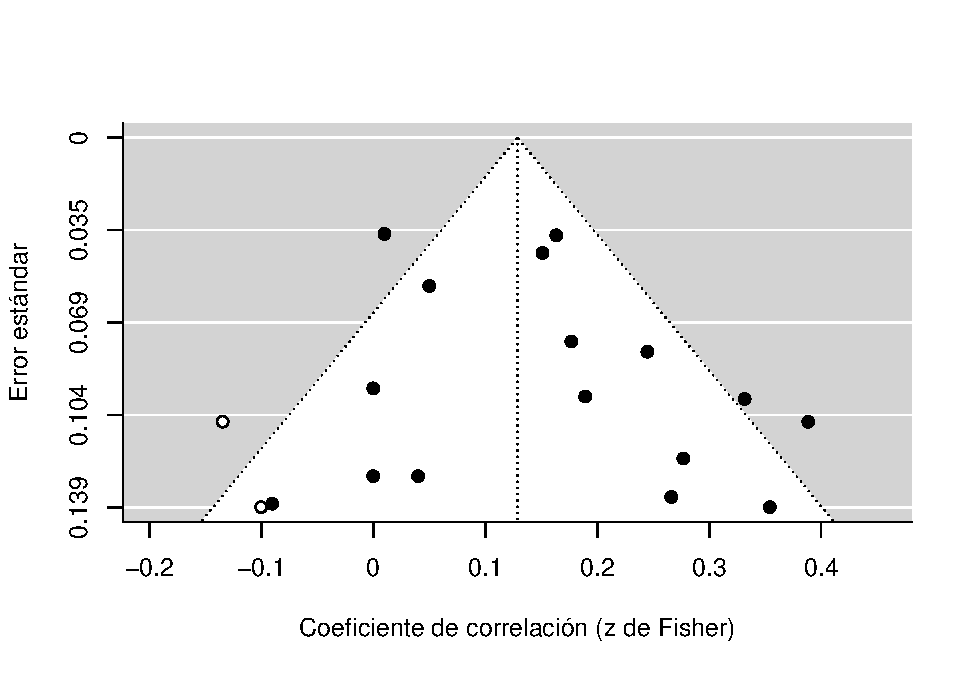
\includegraphics{Meta-analysis_files/figure-latex/tf-plot1-1.pdf}
\caption{\label{fig:tf-plot1}\emph{Funnel plot} básico de \href{https://www.metafor-project.org/doku.php}{metafor} usando el método de recorte y relleno (\emph{trim and fill}). En negro los estudios meta-analizados; en blanco, los estudios \emph{rellenados}.}
\end{figure}

De nuevo, alternativamente podemos usar la función \texttt{viz\_funnel} del paquete \href{https://cran.r-project.org/web/packages/metaviz/vignettes/metaviz.html}{\texttt{metaviz}}, para crear este \emph{funnel plot} representando los estudios \emph{rellenados} con el método de recorte y relleno. Sin embargo, para esto usaremos como argumento el meta-análisis original (\texttt{res}), pero agregando los argumentos \texttt{trim\_and\_fill\ =\ TRUE} y \texttt{trim\_and\_fill\_side\ =\ "left"} (``left'' dado que sabemos que los estudios \emph{faltantes} están a la izquierd).

\begin{Shaded}
\begin{Highlighting}[]
\FunctionTok{viz\_funnel}\NormalTok{(res, }
           \AttributeTok{contours\_col =} \StringTok{"Oranges"}\NormalTok{,}
           \AttributeTok{trim\_and\_fill =} \ConstantTok{TRUE}\NormalTok{, }
           \AttributeTok{trim\_and\_fill\_side =} \StringTok{"left"}\NormalTok{, }\CommentTok{\#IMPORTANTE}
           \AttributeTok{egger =} \ConstantTok{TRUE}\NormalTok{,}
           \AttributeTok{x\_trans\_function =}\NormalTok{ tanh,}
           \AttributeTok{ylab =} \StringTok{"Error estándar"}\NormalTok{,}
           \AttributeTok{xlab =} \StringTok{"Coeficiente de correlación"}\NormalTok{) }\SpecialCharTok{+}
  \FunctionTok{geom\_vline}\NormalTok{(}\AttributeTok{xintercept =} \DecValTok{0}\NormalTok{, }\AttributeTok{linetype =} \StringTok{"dotted"}\NormalTok{)}
\end{Highlighting}
\end{Shaded}

\begin{figure}
\centering
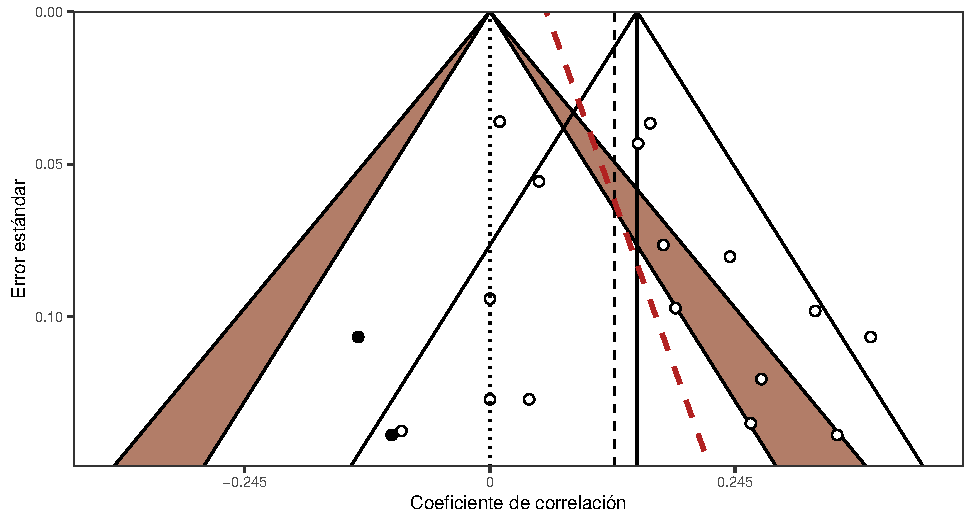
\includegraphics{Meta-analysis_files/figure-latex/tf-plot2-1.pdf}
\caption{\label{fig:tf-plot2}\emph{Funnel plot} creado con \href{https://cran.r-project.org/web/packages/metaviz/vignettes/metaviz.html}{metaviz} usando el método de recorte y relleno (\emph{trim and fill}). En blanco los estudios meta-analizados; en negro, los estudios \emph{rellenados}.}
\end{figure}

El resultado nos muestra que el análisis aumentó dos estudios hipotéticos a la izquierda. Es decir, sugiere que hay \emph{cierto} nivel de sesgo de publicación. De hecho, la estimación del efecto al aumentar estos estudios hipotéticos para que la distribución sea realmente simétrica, disminuye a 0.1288, algo menor que el 0.1499 que nos sugería el análisis inicial.

Si quieres profundizar en el método de recorte y relleno (\emph{trim and fill}), su interpretación, así como sus fortalezas y limitaciones, te recomiendo leer el artículo de Shi \& Lin (\protect\hyperlink{ref-shiTrimandfill2019}{2019}) al respecto.

\hypertarget{vevea-hedges}{%
\subsubsection{Modelo de función de peso de Vevea y Hedges}\label{vevea-hedges}}

El modelo de función de peso de Vevea y Hedges (\protect\hyperlink{ref-veveaGeneralLinearModel1995}{1995}; ver también \protect\hyperlink{ref-veveaPublicationBiasResearch2005}{Vevea \& Woods, 2005}) es uno de los modelos se selección (en inglés, \emph{selection models}) más conocidos\footnote{El otro modelo de selección muy conocido, es el modelo de Copas y Shi (\protect\hyperlink{ref-copasSensitivityAnalysisPublication2001}{2001}, \protect\hyperlink{ref-copasMetaanalysisFunnelPlots2000}{2000}). Aunque no lo incluyo en ésta guía, es importante mencionar que hay evidencia que muestra que es preferible a métodos como el de \emph{trim and fill} (\protect\hyperlink{ref-schwarzerEmpiricalEvaluationSuggests2010}{Schwarzer et al., 2010}). En R, éste método se puede implementar con la función \texttt{copas} del paquete \texttt{metasens} (\protect\hyperlink{ref-schwarzerMetasensPackage}{Schwarzer et al., 2023}; ver también Capítulo 5 en \protect\hyperlink{ref-schwarzerMetaAnalysis2015}{Schwarzer et al., 2015a}).}.

Los modelos de selección intentan describir el mecanismo de supresión del efecto y combinarlo con un modelo de tamaño del efecto que describa la distribución de los efectos en ausencia de sesgo de publicación.

El modelo de Vevea y Hedges da más peso a ciertos tamaños de efecto. La realidad de la literatura científica es que es más probable que algunos estudios sean publicados, dependiendo de sus valores \(p\) (\protect\hyperlink{ref-coburnPublicationBiasFunction2015}{Coburn \& Vevea, 2015}; para una descripción sencilla y general, ver por ejemplo \protect\hyperlink{ref-SesgoPublicacion2008}{Gómez-Restrepo, 2008}). En particular, es más probable que sean publicados los estudios con resultados \emph{significativo} (típicamente, \(p < 0.05\), usando un \(\alpha\) tradicional de 0.05), en comparación con estudios con resultados no significativos (es decir, con resultados que no permiten rechazar la hipótesis nula). Estos sesgos pueden por supuesto sesgar la literatura publicada, y afectar nuestro meta-análisis.

En R, para estimar el sesgo de publicación de un meta-análisis usando el modelo de función de peso de Vevea y Hedges, se puede usar la función \texttt{weightfunct} del paquete \texttt{weightr} (\protect\hyperlink{ref-coburnWeightr2019}{Coburn \& Vevea, 2019}).

Tal como se describe en la \href{https://www.rdocumentation.org/packages/weightr/versions/2.0.2/topics/weightfunct}{documentación} de la función \texttt{weightfunct}, esta función nos permite ``estimar tanto el modelo de función de peso para el sesgo de publicación que se publicó originalmente en Vevea \& Hedges (\protect\hyperlink{ref-veveaGeneralLinearModel1995}{1995}) como la versión modificada presentada en Vevea \& Woods (\protect\hyperlink{ref-veveaPublicationBiasResearch2005}{2005})''.

En este caso, usaré esta función, asignando el resultado a un objeto que llamaré \texttt{wf}.

\begin{Shaded}
\begin{Highlighting}[]
\FunctionTok{library}\NormalTok{(weightr)}
\end{Highlighting}
\end{Shaded}

\begin{verbatim}
Loading required package: scales
\end{verbatim}

\begin{verbatim}

Attaching package: 'scales'
\end{verbatim}

\begin{verbatim}
The following objects are masked from 'package:psych':

    alpha, rescale
\end{verbatim}

\begin{verbatim}
The following object is masked from 'package:purrr':

    discard
\end{verbatim}

\begin{verbatim}
The following object is masked from 'package:readr':

    col_factor
\end{verbatim}

\begin{verbatim}

Attaching package: 'weightr'
\end{verbatim}

\begin{verbatim}
The following object is masked from 'package:metafor':

    funnel
\end{verbatim}

\begin{verbatim}
The following object is masked from 'package:metadat':

    dat.bangertdrowns2004
\end{verbatim}

\begin{verbatim}
The following object is masked from 'package:stats':

    density
\end{verbatim}

\begin{Shaded}
\begin{Highlighting}[]
\NormalTok{wf }\OtherTok{\textless{}{-}} \FunctionTok{weightfunct}\NormalTok{(}\AttributeTok{effect =}\NormalTok{ dat}\SpecialCharTok{$}\NormalTok{yi, }\AttributeTok{v =}\NormalTok{ dat}\SpecialCharTok{$}\NormalTok{vi, }\AttributeTok{table =} \ConstantTok{TRUE}\NormalTok{)}
\NormalTok{wf}
\end{Highlighting}
\end{Shaded}

\begin{ROut}{Consola de R: Output~\thetcbcounter}
                \begin{footnotesize}
                \begin{verbatim} 
Unadjusted Model (k = 16):

tau^2 (estimated amount of total heterogeneity): 0.0070 (SE = 0.0051)
tau (square root of estimated tau^2 value):  0.0834

Test for Heterogeneity:
Q(df = 15) = 38.1595, p-val = 0.001436053

Model Results:

          estimate std.error z-stat      p-val   ci.lb  ci.ub
Intercept   0.1486   0.03073  4.835 1.3288e-06 0.08837 0.2088

Adjusted Model (k = 16):

tau^2 (estimated amount of total heterogeneity): 0.0056 (SE = 0.0045)
tau (square root of estimated tau^2 value):  0.0750

Test for Heterogeneity:
Q(df = 15) = 38.1595, p-val = 0.001436053

Model Results:

              estimate std.error z-stat    p-val    ci.lb  ci.ub
Intercept      0.09153   0.04464  2.050 0.040341  0.00403 0.1790
0.025 < p < 1  0.24121   0.20122  1.199 0.230626 -0.15317 0.6356

Likelihood Ratio Test:
X^2(df = 1) = 2.98493, p-val = 0.084043

Number of Effect Sizes per Interval:

                     Frequency
p-values <0.025              9
0.025 < p-values < 1         7
 \end{verbatim}
                \end{footnotesize}
                \end{ROut}

Los resultados tienen una estructura similar a los del meta-análisis original (descrito y explicado en la sección \ref{meta-cor}) y a los del meta-análisis usando el método \emph{trim and fill} (sección \ref{trim-fill}). Sin embargo, se organizan en dos partes; primero presenta los resultados del modelo no ajustado (bajo el encabezado \texttt{Unadjusted\ Model\ (k\ =\ 16)}), y después presenta los resultados del modelo con pesos ajustados de acuerdo al modelo de función de peso de Vevea y Hedges (bajo el encabezado \texttt{Adjusted\ Model\ (k\ =\ 16)}).

El modelo no ajustado nos da un estimado muy similar (pero no idéntico) al del estudio original (0.1486), dado que usa un método ligeramente diferente.

Como antes, también nos da valores de heterogeneidad \(\tau^2\), \(\tau\) y \(Q\).

Pero lo más importante, es que en la segunda parte (el modelo ajustado) los resultado del meta-análisis se calculan de acuerdo con los pesos dados a cada efecto.

Esta técnica, a diferencia del método \emph{trim and fill} no ``recorta'' ni ``rellena'' estudios, por lo que el análisis se hace con el mismo número de estudios (en este caso, 16; por eso en encabezado dice \texttt{Adjusted\ Model\ (k\ =\ 16)}).

Sin embargo, la función \texttt{weightfunct} incrementa el peso de estudios que tienen menos probabilidad de ser publicados (típicamente resultados no significativos), y reduce el peso de estudios con mayor probabilidad de ser publicados (los que encuentran resultados más extremos). Por esto, al usar ésta técnica, estás asumiendo que, de hecho, en el efecto que tratas de encontrar en tu meta-análisis hay un sesgo de publicación, lo que a menudo es una suposición bastante apropiada.

Al usar ésta técnica, tenemos un resultado bastante distinto. Mientras que el meta-análisis original nos daba como resultado un efecto de \textasciitilde0.15, esta técnica nos estima un efecto de \textasciitilde0.09. Ha \emph{encogido} nuestro tamaño de efecto, asumiendo que nuestro resultado original estaba sesgado.

Al final, está el \emph{Likelihood ratio test} (en español, ``Prueba de la razón de verosimilitud''), que evalúa la bondad del ajuste de dos modelos estadísticos que compiten entre sí, con base en la relación de su verosimilitud\footnote{Aunque no voy a entrar en detalles respecto a técnicas de inferencia estadística basadas en verosimilitud, si quieres conocer más acerca de estos métodos, así como de estadística Bayesiana (que tiene mucho que ver con verosimilitud) y frecuentista (la que solemos usar, que hace inferencia a partir de valores \(p\)), con énfasis en las fortalezas y limitaciones de cada enfoque, recomiendo encarecidamente el libro \emph{``Improving Your Statistical Inferences''} de Daniël Lakens (\protect\hyperlink{ref-lakensImprovingYourStatistical2022}{2022}). Este libro, completamente gratuito y abierto, integra además los contenidos de dos cursos gratuitos del mismo autor (\emph{``\href{https://www.coursera.org/learn/statistical-inferences}{Improving Your Statistical Inferences}''} y \emph{``\href{https://www.coursera.org/learn/improving-statistical-questions}{Improving Your Statistical Questions}''}), que también recomiendo hacer a cualquier persona que quiera dedicarse a hacer investigación y use técnicas estadísticas.}. En este caso, comparando el modelo original, con este modelo con pesos ajustados.

Este resultado nos da una tendencia no descartable (\texttt{p-val\ =\ 0.084043}; menor que 0.10 y por tanto significativa si asumimos un análisis de una cola), que nos da evidencia de que en efecto hay un sesgo de publicación, a pesar de que el \emph{funnel plot} (Figs. \ref{fig:funnel-plot1}, \ref{fig:funnel-plot1a}, \ref{fig:funnel-plot2} y \ref{fig:funnel-plot3}) y la regresión de Egger (sección \ref{reg-egger}), sugerían lo contrario.

\hypertarget{poder-inf}{%
\subsection{Poder estadístico del meta-análisis}\label{poder-inf}}

En esta sección explicaré cómo hacer un análisis de poder de un meta-análisis.
Como mencioné anteriormente, de ser necesario, para entender las bases del poder estadístico, recomiendo ver \href{https://youtube.com/playlist?list\%20=\%20PLHk7UNt35ccVdyHqnQ6oXVYA6JBNFrE1x}{esta serie de videos} (\protect\hyperlink{ref-leongomezPoderRvid2020}{Leongómez, 2020b}) y/o, para mayor profundidad, leer \href{https://doi.org/10.5281/zenodo.3988776}{esta guía} (\protect\hyperlink{ref-leongomezAnalisisPoderEstadistico2020}{Leongómez, 2020a}) que publiqué anteriormente.

La idea de ésto es saber si nuestro meta-análisis tiene un poder suficiente para detectar el efecto \emph{real} estimado mediante nuestro análisis (en nuestro caso \emph{z} = 0.15 para el meta-análisis original ``\texttt{res}'', o \emph{z} = 0.09 el meta-análisis con pesos ajustados ``\texttt{wf}'').

Para este ejemplo, asumiré que el efecto \emph{real} es el estimado en nuestro análisis original (\emph{z} = 0.15), pues este efecto es mayor. Si no tuviésemos el poder suficiente para detectar confiablemente ese efecto, menos lo tendríamos para un efecto menor, como el detectado en nuestro meta-análisis con pesos ajustados.

Para hacer esto, usaré el paquete \texttt{metameta} (\protect\hyperlink{ref-quintanaMetameta2022}{Quintana, 2022}, \protect\hyperlink{ref-quintanaGuideMetaPower}{2023}), que permite calcular y visualizar el poder estadístico de un meta-análisis para detectar un rango de posibles efectos \emph{reales} estimados.

\hypertarget{instalaciuxf3n-de-metameta}{%
\subsubsection{\texorpdfstring{Instalación de \texttt{metameta}}{Instalación de metameta}}\label{instalaciuxf3n-de-metameta}}

El paquete \texttt{metameta} se debe instalar desde GitHub ya que, al día de hoy, no está aún disponible en CRAN\footnote{\href{https://cran.r-project.org/}{CRAN} (siglas de \emph{Comprehensive R Archive Network}) es una red de servidores de todo el mundo que almacenan versiones idénticas y actualizadas del código y la documentación de R (incluyendo el lenguaje mismo de R, paquetes aceptados por el equipo de CRAN, y toda la documentación). Es el repositorio oficial y dedicado a R, desde el que normalmente instalas cualquier paquete. \href{https://github.com/}{GitHub}, en cambio, es un repositorio general y abierto para para proyectos (típicamente programación) en el que, entre otras cosas, suelen estar alojados todos los paquetes de R en versiones de desarrollador, y antes de ser aceptados en CRAN. Por supuesto, a diferencia de CRAN, GitHub es un repositorio de código general, no específico para R.}.

Para esto, debemos tener instalado el paquete \texttt{devtools}, y usar la función \texttt{install\_github} que nos permite instalar paquetes directamente desde GitHub.

\begin{Shaded}
\begin{Highlighting}[]
\CommentTok{\#se debe tener instalado el paquete devtools}
\FunctionTok{library}\NormalTok{(devtools)}
\FunctionTok{install\_github}\NormalTok{(}\StringTok{"dsquintana/metameta"}\NormalTok{)}
\end{Highlighting}
\end{Shaded}

\hypertarget{anuxe1lisis-de-poder}{%
\subsubsection{Análisis de poder}\label{anuxe1lisis-de-poder}}

Una vez hemos instalado \texttt{metameta}, podemos cargar el paquete.

\begin{Shaded}
\begin{Highlighting}[]
\FunctionTok{library}\NormalTok{(metameta)}
\end{Highlighting}
\end{Shaded}

Como datos, necesitamos no solamente los tamaños de efecto a meta-analizar (\(r\) de Pearson transformado a \emph{z} de Fisher), sino además los intervalos de confianza, tal como fueron reportados en varios de nuestros \emph{Forest plots}.

Como mencioné, voy a asumir un efecto \emph{real} de \(r = 0.15\), tal como en nuestro meta-análisis original. Sin embargo, el efecto \emph{real} no es algo que podamos saber con absoluta certeza (es, de hecho, lo que queremos acercarnos a conocer a través del meta-análisis), así que la función \texttt{mapower\_ul} del paquete \texttt{metameta} calcula el poder de cada meta-análisis para un rango de posibles efectos reales.

Para esto, la función \texttt{mapower\_ul} requiere una base de datos que contenga información concreta, y con columnas con nombres específicos: el efecto encontrado en cada estudio (en nuestro caso \texttt{yi}, que es la columna en la que guardamos los coeficientes de correlación transformados a \emph{z} de Fisher), así como sus intervalos de confianza. Estas columnas deben llamarse \texttt{yi}, \texttt{lower} y \texttt{upper}, respectivamente.

Esto lo puedo obtener de manera sencilla con la función \texttt{summary}, que agrega a la base de datos (\texttt{dat}) los límites inferior (\texttt{ci.lb}) y superior (\texttt{ci.ub}) de los intervalos de confianza. Sin embargo, aunque la columna con el tamaño de efecto (\texttt{yi}) ya tiene el nombre requerido, debo renombrar las columnas que tienen los límites de los intervalos de confianza (\texttt{ci.lb} y \texttt{ci.ub}) como \texttt{lower} y \texttt{upper}, usando la función \texttt{rename}.

\begin{Shaded}
\begin{Highlighting}[]
\NormalTok{dat.poder }\OtherTok{\textless{}{-}} \FunctionTok{summary}\NormalTok{(dat) }\SpecialCharTok{\%\textgreater{}\%}
  \FunctionTok{rename}\NormalTok{(}\AttributeTok{lower =}\NormalTok{ ci.lb, }\AttributeTok{upper =}\NormalTok{ ci.ub)}
\end{Highlighting}
\end{Shaded}

Asigné esta versión modificada de la base de datos a un objeto que llamé \texttt{dat.poder}. Ya con esta base de datos lista y con el formato correcto para usar la función \texttt{mapower\_ul}, podemos seguir adelante.

La función \texttt{mapower\_ul} requiere que asignemos la base de datos (\texttt{dat.poder}) al argumento \texttt{dat}, el tamaño de efecto que estimamos como efecto \emph{real} (en este caso, 0.15) al argumento \texttt{observed\_es}, así como un nombre que le daremos al meta-análisis al argumento \texttt{name} (en este caso lo llamaré ``Molloy et al.~2014'', pero por supuesto tú puedes darle el nombre que consideres adecuado, siempre entre comillas). Asignaré el resultado de este análisis a un objeto que simplemente llamaré \texttt{poder}.

\begin{Shaded}
\begin{Highlighting}[]
\NormalTok{poder }\OtherTok{\textless{}{-}} \FunctionTok{mapower\_ul}\NormalTok{(}\AttributeTok{dat =}\NormalTok{ dat.poder, }\AttributeTok{observed\_es =} \FloatTok{0.15}\NormalTok{, }\AttributeTok{name =} \StringTok{"Molloy et al. 2014"}\NormalTok{)}
\end{Highlighting}
\end{Shaded}

Como veremos a continuación, éste objeto tiene varios elementos muy importantes.

\hypertarget{poder-mediano}{%
\paragraph{Poder mediano del meta-análisis para diferentes tamaños de efecto.}\label{poder-mediano}}

El objeto generado por la función \texttt{mapower\_ul} tiene varios elementos. Uno particularmente relevante es la lista de poder mediano estimado para diferentes tamaños de efecto (\texttt{\$power\_median\_dat}), que asignaré como lista a un objeto que llamaré \texttt{lista\_poder} (guardar este objeto es sumamente útil para hacer visualizaciones del análisis de poder, como explico más adelante, en la sección \ref{firepower-plot}).

\begin{Shaded}
\begin{Highlighting}[]
\NormalTok{lista\_poder }\OtherTok{\textless{}{-}} \FunctionTok{list}\NormalTok{(poder}\SpecialCharTok{$}\NormalTok{power\_median\_dat)}
\end{Highlighting}
\end{Shaded}

Para ver el objeto, como siempre, solo tengo que llamarlo por el nombre que le haya dado (en este caso, \texttt{lista\_poder}). Muestra el poder estadístico del meta-análisis para detectar diferentes tamaños de efecto (que llama \texttt{es}, por las siglas en inglés de \emph{effect size}).

\begin{Shaded}
\begin{Highlighting}[]
\NormalTok{lista\_poder}
\end{Highlighting}
\end{Shaded}

\begin{ROut}{Consola de R: Output~\thetcbcounter}
                \begin{footnotesize}
                \begin{verbatim} [[1]]
  power_es_observed      es01      es02      es03      es04      es05      es06
1                 0 0.1762492 0.5356629 0.8673657 0.9837594 0.9992182 0.9999858
       es07 es08 es09 es1 es_observed meta_analysis_name
1 0.9999999    1    1   1   0.3364197 Molloy et al. 2014
 \end{verbatim}
                \end{footnotesize}
                \end{ROut}

Por ejemplo, nos muestra que para detectar un efecto de \emph{z} = 0.1 (\texttt{es01}), se estima un poder de \texttt{0.1762492}; para un poder de \emph{z} = 0.2 (\texttt{es02}), se estima un poder de \texttt{0.5356629}, y continúa así hasta un poder de \emph{z} = 1.0 (\texttt{es1}).

Finalmente, nos muestra el poder estimado para detectar un efecto del tamaño del que estimamos como \emph{real} (en nuestro caso, \emph{z} = 0.15), bajo el encabezado \texttt{es\_observed}. Como se ve, el poder es de tan solo \texttt{0.3364197}, lo que quiere decir que, si el efecto \emph{real} de la asociación entre escrupulosidad y la adherencia a la medicación fuese \emph{z} = 0.15, un meta-análisis como el nuestro sólo detectaría esa correlación como significativa en el 33.64\% de os casos.

Lo que es más, podemos concluir que solo tenemos suficiente poder estadístico para detectar como significativos efectos desde aproximadamente \emph{z} = 0.3 (\texttt{es03} = \texttt{0.8673657}, donde por fin tenemos un poder mayor a 0.8, o lo que es lo mismo, 80\%). Sin embargo, nuestras estimaciones del efecto \emph{real} están por debajo de este umbral, ya que en nuestro meta-análisis original fue de \emph{z} = 0.15 y en el meta-análisis con pesos ajustados fue de \emph{z} = 0.09.

\hypertarget{poder-de-cada-estudio-para-diferentes-tamauxf1os-de-efecto.}{%
\paragraph{Poder de cada estudio para diferentes tamaños de efecto.}\label{poder-de-cada-estudio-para-diferentes-tamauxf1os-de-efecto.}}

El otro elemento generado es una base de datos modificada que, de manera similar a la lista de poder mediano, contiene el poder estimado para diferentes tamaños de efecto, pero en este caso no como una mediana, sino para cada estudio (\texttt{\$dat}). Asignaré este elemento a un objeto que llamaré \texttt{poder\_full\_dat}.

\begin{Shaded}
\begin{Highlighting}[]
\NormalTok{poder\_full\_dat }\OtherTok{\textless{}{-}}\NormalTok{ poder}\SpecialCharTok{$}\NormalTok{dat}
\NormalTok{poder\_full\_dat}
\end{Highlighting}
\end{Shaded}

\begin{ROut}{Consola de R: Output~\thetcbcounter}
                \begin{footnotesize}
                \begin{verbatim}    study_id             authors year  ni     ri controls          design
1         1     Axelsson et al. 2009 109  0.187     none cross-sectional
2         2     Axelsson et al. 2011 749  0.162     none cross-sectional
3         3        Bruce et al. 2010  55  0.340     none     prospective
4         4  Christensen et al. 1999 107  0.320     none cross-sectional
5         5 Christensen & Smith 1995  72  0.270     none     prospective
6         6        Cohen et al. 2004  65  0.000     none     prospective
7         7      Dobbels et al. 2005 174  0.175     none cross-sectional
8         8       Ediger et al. 2007 326  0.050 multiple     prospective
9         9        Insel et al. 2006  58  0.260     none     prospective
10       10       Jerant et al. 2011 771  0.010 multiple     prospective
11       11        Moran et al. 1997  56 -0.090 multiple     prospective
12       12   O'Cleirigh et al. 2007  91  0.370     none     prospective
13       13       Penedo et al. 2003 116  0.000     none cross-sectional
14       14        Quine et al. 2012 537  0.150     none     prospective
15       15      Stilley et al. 2004 158  0.240     none     prospective
16       16 Wiebe & Christensen 1997  65  0.040     none     prospective
     a_measure c_measure meanage quality          yi          vi        sei
1  self-report     other   22.00       1  0.18922664 0.009433962 0.09712680
2  self-report       NEO   53.59       1  0.16343992 0.001340483 0.03661193
3        other       NEO   43.36       2  0.35409253 0.019230769 0.13867250
4  self-report     other   41.70       1  0.33164711 0.009615385 0.09805627
5        other       NEO   46.39       2  0.27686382 0.014492754 0.12038364
6        other       NEO   41.20       2  0.00000000 0.016129032 0.12699779
7  self-report       NEO   52.30       1  0.17682002 0.005847953 0.07647051
8  self-report       NEO   41.00       3  0.05004173 0.003095975 0.05564047
9        other     other   77.00       2  0.26610841 0.018181818 0.13483749
10       other       NEO   78.60       3  0.01000033 0.001302083 0.03608373
11       other       NEO   57.20       2 -0.09024419 0.018867925 0.13735804
12 self-report       NEO   37.90       2  0.38842310 0.011363636 0.10659840
13 self-report       NEO   39.20       1  0.00000000 0.008849558 0.09407036
14 self-report     other   69.00       2  0.15114044 0.001872659 0.04327344
15       other       NEO   46.20       3  0.24477411 0.006451613 0.08032046
16       other       NEO   56.00       1  0.04002135 0.016129032 0.12699779
           zi         pval        lower      upper power_es_observed power_es01
1   1.9482075 5.139014e-02 -0.001141888 0.37959517         0.3390835  0.1774836
2   4.4640346 8.043057e-06  0.091680539 0.23519930         0.9837035  0.7797623
3   2.5533975 1.066777e-02  0.082294427 0.62589063         0.1910727  0.1113715
4   3.3821502 7.192082e-04  0.139456828 0.52383739         0.3337559  0.1750148
5   2.2998036 2.145935e-02  0.040911886 0.51281576         0.2383028  0.1320187
6   0.0000000 1.000000e+00 -0.248915675 0.24891567         0.2188783  0.1234921
7   2.3122218 2.076546e-02  0.026937828 0.32670221         0.5006730  0.2576556
8   0.8993600 3.684609e-01 -0.059013584 0.15909704         0.7691106  0.4354589
9   1.9735128 4.843717e-02  0.001826917 0.53038990         0.1994161  0.1149996
10  0.2771374 7.816746e-01 -0.060723775 0.08072444         0.9859910  0.7914240
11 -0.6569876 5.111889e-01 -0.359465946 0.17897757         0.1938536  0.1125800
12  3.6437317 2.687136e-04  0.179490237 0.59735596         0.2905754  0.1553001
13  0.0000000 1.000000e+00 -0.184377902 0.18437790         0.3575910  0.1861296
14  3.4926197 4.783072e-04  0.066324499 0.23595637         0.9340134  0.6371865
15  3.0474131 2.308202e-03  0.087346017 0.40220221         0.4632371  0.2379950
16  0.3151285 7.526641e-01 -0.208894321 0.28893703         0.2188783  0.1234921
   power_es02 power_es03 power_es04 power_es05 power_es06 power_es07 power_es08
1   0.5395394  0.8705053  0.9845502  0.9992836  0.9999877  0.9999999  1.0000000
2   0.9997697  1.0000000  1.0000000  1.0000000  1.0000000  1.0000000  1.0000000
3   0.3026621  0.5806100  0.8223954  0.9500825  0.9910281  0.9989921  0.9999302
4   0.5317864  0.8642261  0.9829686  0.9991528  0.9999840  0.9999999  1.0000000
5   0.3827659  0.7026651  0.9135189  0.9858616  0.9987531  0.9999421  0.9999986
6   0.3502733  0.6562694  0.8829174  0.9759855  0.9971497  0.9998088  0.9999929
7   0.7439048  0.9751837  0.9994638  0.9999977  1.0000000  1.0000000  1.0000000
8   0.9489275  0.9997002  0.9999999  1.0000000  1.0000000  1.0000000  1.0000000
9   0.3170763  0.6044851  0.8429297  0.9597856  0.9936099  0.9993842  0.9999645
10  0.9998300  1.0000000  1.0000000  1.0000000  1.0000000  1.0000000  1.0000000
11  0.3074782  0.5886809  0.8294859  0.9535367  0.9919839  0.9991443  0.9999443
12  0.4666848  0.8035418  0.9634686  0.9968384  0.9998781  0.9999980  1.0000000
13  0.5659845  0.8904902  0.9890522  0.9996035  0.9999950  1.0000000  1.0000000
14  0.9961139  0.9999997  1.0000000  1.0000000  1.0000000  1.0000000  1.0000000
15  0.7019697  0.9620572  0.9987365  0.9999900  1.0000000  1.0000000  1.0000000
16  0.3502733  0.6562694  0.8829174  0.9759855  0.9971497  0.9998088  0.9999929
   power_es09 power_es1
1   1.0000000 1.0000000
2   1.0000000 1.0000000
3   0.9999971 0.9999999
4   1.0000000 1.0000000
5   1.0000000 1.0000000
6   0.9999999 1.0000000
7   1.0000000 1.0000000
8   1.0000000 1.0000000
9   0.9999988 1.0000000
10  1.0000000 1.0000000
11  0.9999978 0.9999999
12  1.0000000 1.0000000
13  1.0000000 1.0000000
14  1.0000000 1.0000000
15  1.0000000 1.0000000
16  0.9999999 1.0000000
 \end{verbatim}
                \end{footnotesize}
                \end{ROut}

Básicamente, esta tabla contiene información nos permite evaluar si cada estudio incluido en nuestro meta-análisis tenía o no un poder estadístico suficiente para detectar un rango de tamaños de efecto que, como antes van desde \emph{z} = 0.1 (columna \texttt{power\_es01}), hasta \emph{z} = 1.0 (\texttt{power\_es1}).

También, nos permite ver el poder estadístico de cada estudio para detectar un tamaño de efecto \emph{real} como el que estimamos (\emph{z} = 0.15), en la columna \texttt{power\_es\_observed} (la información de esta columna es análoga a la de los \emph{funnel plot} creados con la función \texttt{viz\_funnel} del paquete \texttt{metaviz}; Fig. \ref{fig:funnel-plot3}A y B).

\hypertarget{firepower-plot}{%
\subsubsection{\texorpdfstring{Visualización del análisis de poder (\emph{Firepower plot})}{Visualización del análisis de poder (Firepower plot)}}\label{firepower-plot}}

Estos análisis muestran que, en promedio, nuestro meta-análisis sólo alcanza un poder estadístico suficiente (mayor a 0.8 u 80\%) para detectar de manera confiable efectos mayores a \textasciitilde0.3, lo que está muy por encima de nuestras estimaciones del efecto real (0.15 en nuestro meta-análisis original, 0.09 en nuestro meta-análisis con pesos ajustados). De hecho, el poder estimado para detectar un efecto de 0.15 es de apenas 33.64\% (reportado como \texttt{es\_observed}, con un valor de \texttt{0.3364197} en el Output 10 de la sección \ref{poder-mediano}).

Puedo fácilmente crear una visualización de esto con la función \texttt{firepower} del paquete \texttt{metameta}. Solo tengo que agregar, como único argumento, el objeto en el que guardé la lista de poder mediano estimado para diferentes tamaños de efecto (que en este caso asigné a un objeto que llamé \texttt{lista\_poder} en la sección \ref{poder-mediano}).

\begin{Shaded}
\begin{Highlighting}[]
\NormalTok{poder.plot }\OtherTok{\textless{}{-}} \FunctionTok{firepower}\NormalTok{(lista\_poder)}
\end{Highlighting}
\end{Shaded}

En este caso asigné el \emph{fireplot} resultante a un objeto, para poder modificar después, que llamé \texttt{poder.plot}. Para verlo, entonces, debo correr el objeto para ver el resultado (Fig. \ref{fig:fire-plot1}).

\begin{Shaded}
\begin{Highlighting}[]
\NormalTok{poder.plot}
\end{Highlighting}
\end{Shaded}

\begin{figure}
\centering
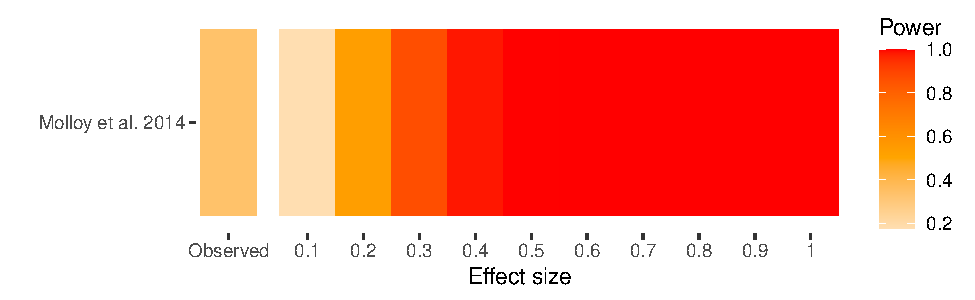
\includegraphics{Meta-analysis_files/figure-latex/fire-plot1-1.pdf}
\caption{\label{fig:fire-plot1}Fireplot básico de \href{https://www.dsquintana.blog/metameta-r-package-meta-analysis/}{metameta}, para un análisis de poder de nuestro meta-análisis. \emph{Observed} hace referencia al tamaño de efecto observado en nuestro meta-análisis original; en este caso, 0.15.}
\end{figure}

El objeto \texttt{poder.plot} contiene dos elementos: los datos (\texttt{\$dat}) y la gráfica propiamente dicha (\texttt{\$fp\_plot}). Éste último elemento es de clase \texttt{ggplot}, por lo que podemos usar funciones de \texttt{ggplot2} para cambiar, por ejemplo, el título del eje \(X\) a ``Tamaño de efecto'', el título de la leyenda a ``Poder'', y el efecto observado de ``\emph{Observed}'' a ``Observado''\footnote{Para cambiar el título del eje \(X\) usé la función \texttt{xlab}; para el título de la leyenda la función \texttt{guides} (opción \texttt{fill\ =\ guide\_legend}); y para los valores del eje \(X\), la función \texttt{scale\_x\_discrete}\}.}. Por ejemplo:

\begin{Shaded}
\begin{Highlighting}[]
\NormalTok{poder.plot}\SpecialCharTok{$}\NormalTok{fp\_plot }\SpecialCharTok{+}
  \FunctionTok{xlab}\NormalTok{(}\StringTok{"Tamaño de efecto"}\NormalTok{) }\SpecialCharTok{+}
  \FunctionTok{guides}\NormalTok{(}\AttributeTok{fill =} \FunctionTok{guide\_legend}\NormalTok{(}\AttributeTok{title =} \StringTok{"Poder"}\NormalTok{, }
                             \AttributeTok{reverse =} \ConstantTok{TRUE}\NormalTok{)) }\SpecialCharTok{+}
  \FunctionTok{scale\_x\_discrete}\NormalTok{(}\AttributeTok{labels =} \FunctionTok{c}\NormalTok{(}\StringTok{"es\_observed"} \OtherTok{=} \StringTok{"Observado"}\NormalTok{,}
                              \StringTok{"es01"} \OtherTok{=} \FloatTok{0.1}\NormalTok{, }\StringTok{"es02"} \OtherTok{=} \FloatTok{0.2}\NormalTok{, }\StringTok{"es03"} \OtherTok{=} \FloatTok{0.3}\NormalTok{, }\StringTok{"es04"} \OtherTok{=} \FloatTok{0.4}\NormalTok{, }
                              \StringTok{"es05"} \OtherTok{=} \FloatTok{0.5}\NormalTok{, }\StringTok{"es06"} \OtherTok{=} \FloatTok{0.6}\NormalTok{, }\StringTok{"es07"} \OtherTok{=} \FloatTok{0.7}\NormalTok{, }\StringTok{"es08"} \OtherTok{=} \FloatTok{0.8}\NormalTok{, }
                              \StringTok{"es09"} \OtherTok{=} \FloatTok{0.9}\NormalTok{, }\StringTok{"es1"}  \OtherTok{=} \DecValTok{1}\NormalTok{))}
\end{Highlighting}
\end{Shaded}

Este código produce la Figura \ref{fig:fire-plot2}, con todos los textos en español.

\begin{figure}
\centering
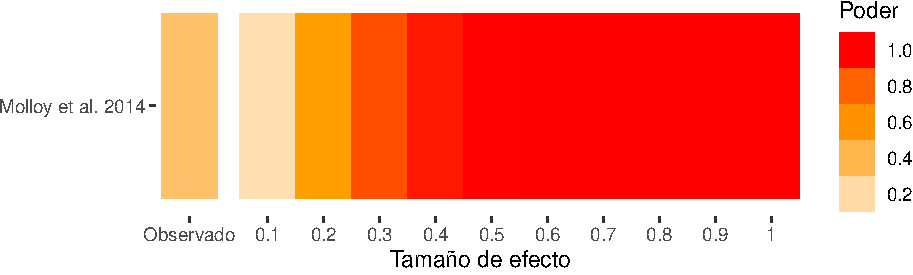
\includegraphics{Meta-analysis_files/figure-latex/fire-plot2-1.pdf}
\caption{\label{fig:fire-plot2}Fireplot básico de \href{https://www.dsquintana.blog/metameta-r-package-meta-analysis/}{metameta}, para un análisis de poder de nuestro meta-análisis, con el texto traducido a español y con la leyenda en una escala discreta para facilitar su lectura. \emph{Observado} hace referencia al tamaño de efecto observado en nuestro meta-análisis original (en este caso, 0.15).}
\end{figure}

La Figura \ref{fig:fire-plot2} nos permite comprobar, de nuevo, que el meta-análisis solamente alcanza un poder mínimo recomendado de 0.8 (80\%) cuando se trata de efectos de \emph{z} = 0.3 (o mayores), y que para nuestro efecto \emph{observado} (\emph{z} = 0.15), el poder apenas alcanza cerca de 0.4 (40\%).

Si el poder estadístico de nuestro meta-análisis para detectar ese efecto (\emph{z} = 0.15) es demasiado bajo, por supuesto sería aún más deficiente para detectar un efecto menor, como el estimado en nuestro modelo con pesos corregidos (\emph{z} = 0.09).

\hypertarget{todas-combinaciones}{%
\subsection{Más información sobre influencia y meta-análisis combinatorio}\label{todas-combinaciones}}

Como hemos visto, al realizar un meta-análisis, es fundamental tomar decisiones que pueden influir significativamente en los resultados y conclusiones. Una de las preguntas más importantes es qué estudios incluir en el análisis y si es necesario excluir algún estudio. Aunque nuestro diagnóstico inicial de influencia (sección \ref{diag-inf}) no mostró la presencia de estudios atípicos en nuestro meta-análisis, en ocasiones se requiere un análisis más exhaustivo.

En esta sección, que se basa por completo en la explicación y ejemplos de Quintana (\protect\hyperlink{ref-quintanaOhMyGOSH2020}{2020}), explicaré dos técnicas: \emph{leave-one-out} (sección \ref{leave-one-out}), que consiste en realizar una serie de meta-análisis excluyendo uno de los estudios incluidos en cada iteración, y meta-análisis combinatorio (sección \ref{gosh}), que permite crear todas las combinaciones posibles de estudios y, por lo tanto, evaluar la robustez de los resultados en diferentes escenarios.

\hypertarget{leave-one-out}{%
\subsubsection{\texorpdfstring{\emph{Leave-one-out}}{Leave-one-out}}\label{leave-one-out}}

La técnica de \emph{leave-one-out} realiza una serie de meta-análisis dejando fuera cada uno de los estudios incluidos. En nuestro caso, dado que tenemos 16 estudios, esta técnica ajustará 16 modelos (uno excluyendo cada estudio).

Esta técnica no sólo se puede hacer como parte de un diagnóstico de influencia (como se muestra en la sección \ref{diag-inf}), sino que también se puede hacer para ver la estimación del efecto meta-analizado al excluir cada uno de los estudios de nuestra base de datos.

Hacerlo sólo requiere usar la función \texttt{leave1out} del paquete \texttt{metafor}, usando como argumento el resultado de nuestro meta-análisis original (en este caso, \texttt{res}):

\begin{Shaded}
\begin{Highlighting}[]
\FunctionTok{leave1out}\NormalTok{(res)}
\end{Highlighting}
\end{Shaded}

\begin{ROut}{Consola de R: Output~\thetcbcounter}
                \begin{footnotesize}
                \begin{verbatim} 
   estimate     se   zval   pval  ci.lb  ci.ub       Q     Qp   tau2      I2 
1    0.1483 0.0336 4.4157 0.0000 0.0825 0.2142 37.7109 0.0006 0.0091 64.9684 
2    0.1500 0.0354 4.2355 0.0000 0.0806 0.2194 36.7672 0.0008 0.0100 62.2717 
3    0.1418 0.0315 4.5064 0.0000 0.0801 0.2035 35.3930 0.0013 0.0075 61.1741 
4    0.1379 0.0308 4.4739 0.0000 0.0775 0.1984 33.5886 0.0024 0.0068 58.1050 
5    0.1441 0.0323 4.4550 0.0000 0.0807 0.2075 36.5396 0.0009 0.0082 62.8995 
6    0.1566 0.0326 4.8119 0.0000 0.0928 0.2205 37.1703 0.0007 0.0084 63.5769 
7    0.1489 0.0342 4.3555 0.0000 0.0819 0.2160 37.6797 0.0006 0.0094 65.1901 
8    0.1599 0.0334 4.7841 0.0000 0.0944 0.2254 36.1484 0.0010 0.0084 61.4011 
9    0.1455 0.0324 4.4863 0.0000 0.0819 0.2091 37.0495 0.0007 0.0083 63.4803 
10   0.1647 0.0291 5.6601 0.0000 0.1077 0.2218 25.0661 0.0339 0.0047 43.6587 
11   0.1586 0.0317 5.0069 0.0000 0.0965 0.2207 35.6617 0.0012 0.0077 61.6732 
12   0.1353 0.0296 4.5647 0.0000 0.0772 0.1934 31.9021 0.0041 0.0059 55.0102 
13   0.1592 0.0324 4.9100 0.0000 0.0956 0.2227 36.3291 0.0009 0.0080 62.0683 
14   0.1514 0.0353 4.2858 0.0000 0.0821 0.2206 37.7339 0.0006 0.0100 63.6942 
15   0.1432 0.0330 4.3432 0.0000 0.0786 0.2078 35.8385 0.0011 0.0083 62.6114 
16   0.1552 0.0329 4.7203 0.0000 0.0908 0.2196 37.7017 0.0006 0.0087 64.3368 
       H2 
1  2.8546 
2  2.6505 
3  2.5756 
4  2.3869 
5  2.6954 
6  2.7455 
7  2.8727 
8  2.5907 
9  2.7382 
10 1.7749 
11 2.6091 
12 2.2227 
13 2.6363 
14 2.7544 
15 2.6746 
16 2.8040 
 \end{verbatim}
                \end{footnotesize}
                \end{ROut}

Como puedes ver, esta función crea una tabla con las columnas \texttt{estimate}, \texttt{se}, \texttt{zval}, \texttt{pval}, \texttt{ci.lb}, \texttt{ci.ub}, \texttt{Q}, \texttt{Qp}, \texttt{tau2}, \texttt{I2} y \texttt{H2} (explicadas en la sección \ref{meta-interp}). Sin embargo, tenemos 16 filas, cada una de las cuales corresponde a los resultados cuando se excluye ese estudio del meta-análisis.

En este caso, los tamaños del efecto estimado (columna \texttt{estimate}) para los meta-análisis que eliminaron un único estudio están entre \emph{z} = 0.14 y \emph{z} = 0.16, lo que muestra que la eliminación de un estudio no influye mucho en el tamaño del efecto original estimado, que fue de \emph{z} = 0.15. En otras palabras, podríamos eliminar cualquier estudio de nuestro análisis y el resultado cambiaría muy poco.

Aunque este análisis es bastante informativo, podría haber un subgrupo de estudios ---en lugar de un único estudio--- que influye en el resultado. Para investigar esto, podemos hacer un meta-análisis combinatorio.

\hypertarget{gosh}{%
\subsubsection{Meta-análisis combinatorio}\label{gosh}}

Aunque la técnica de \emph{leave-one-out} es útil para determinar la influencia de cada estudio en un meta-análisis, no nos dice nada de cuánto cambia nuestra estimación del efecto real cuando excluimos dos o más estudios. Por lo tanto, el meta-análisis combinatorio puede ser una técnica complementaria para detectar subgrupos de estudios que estén afectando nuestros resultados

Por ejemplo, si estamos realizando un meta-análisis sobre el efecto del consumo de café en la salud cardiovascular, es posible que encontremos varios estudios que no controlan adecuadamente el consumo de tabaco de los participantes. Si eliminamos uno solo de estos estudios, es posible que aún quede un sesgo importante en nuestra estimación del efecto \emph{real}. En este caso, el meta-análisis combinatorio nos permitiría evaluar todas las posibles combinaciones de estudios que incluyen o excluyen los estudios que no controlan el consumo de tabaco, lo que nos ayudaría a comprender mejor el impacto de estos estudios en nuestra estimación del efecto \emph{real}.

Un meta-análisis combinatorio ajusta una serie de meta-análisis a partir de todas las combinaciones posibles de estudios. Esta técnica es poderosa, pero es importante tener en cuenta que el número de posibles combinaciones aumenta exponencialmente a medida que aumenta el número de estudios incluidos en nuestro meta-análisis. De hecho, el número de análisis a realizar puede calcularse usando la fórmula \(2^k - 1\), donde \(k\) es el número de estudios meta-analizados (Tabla \ref{tab:gosh-combs}).

\begin{table}[H]

\caption{\label{tab:gosh-combs}Número de posibles combinaciones según número de estudios (k)}
\centering
\begin{tabular}[t]{>{}c>{}r|>{}cr}
\toprule
\multicolumn{1}{c}{\makecell[c]{Número de\\estudios\\(\textit{k})}} & \multicolumn{1}{c}{\makecell[c]{Posibles\\combinaciones\\($2^{k} - 1$)}} & \multicolumn{1}{c}{\makecell[c]{Número de\\estudios\\(\textit{k})}} & \multicolumn{1}{c}{\makecell[c]{Posibles\\combinaciones\\($2^{k} - 1$)}}\\
\midrule
\textbf{5} & 31 & \textbf{18} & 262 143\\
\textbf{6} & 63 & \textbf{19} & 524 287\\
\textbf{7} & 127 & \textbf{20} & 1 048 575\\
\textbf{8} & 255 & \textbf{21} & 2 097 151\\
\textbf{9} & 511 & \textbf{22} & 4 194 303\\
\textbf{10} & 1 023 & \textbf{23} & 8 388 607\\
\textbf{11} & 2 047 & \textbf{24} & 16 777 215\\
\textbf{12} & 4 095 & \textbf{25} & 33 554 431\\
\textbf{13} & 8 191 & \textbf{26} & 67 108 863\\
\textbf{14} & 16 383 & \textbf{27} & 134 217 727\\
\textbf{15} & 32 767 & \textbf{28} & 268 435 455\\
\textbf{16} & 65 535 & \textbf{29} & 536 870 911\\
\textbf{17} & 131 071 & \textbf{30} & 1 073 741 823\\
\bottomrule
\end{tabular}
\end{table}

Como se puede ver en la Tabla \ref{tab:gosh-combs}, el número de combinaciones aumenta drásticamente a medida que aumenta el número de estudios en nuestro meta-análisis. Por ejemplo, si tuviéramos 5 estudios, habría solo 31 posibles combinaciones (\(2^{5} - 1\) = 31). Sin embargo, si tuviéramos 20 estudios, habría más de un millón de combinaciones (\(2^{16} - 1\) = 1 048 575) y si tuviéramos 30 estudios, habría más de mil millones de combinaciones (ver Tabla \ref{tab:gosh-combs}). Dado que esto puede consumir muchos recursos computacionales, es importante tener precaución al realizar un meta-análisis combinatorio con un gran número de estudios. El análisis puede tardar mucho tiempo e incluso fallar si se usa toda la memoria RAM del ordenador.

En nuestro ejemplo, estamos meta-analizando 16 estudios, lo que significa que necesitamos ajustar 65 535 modelos (\(2^{16} - 1\)). Ajustar todos estos modelos puede llevar bastante tiempo, aunque esto dependerá de las especificaciones de tu equipo (en mi portátil, tarda alrededor de 5 minutos).

Para visualizar la heterogeneidad entre los estudios, podemos utilizar una técnica llamada \emph{visualización gráfica de la heterogeneidad de los estudios} (en inglés, \emph{Graphical Display of Study Heterogeneity} o simplemente \emph{GOSH}), propuesta por Olkin et al. (\protect\hyperlink{ref-olkinGOSHGraphicalDisplay2012}{2012}). En R, podemos realizar esta visualización utilizando la función \texttt{gosh} del paquete \texttt{metafor}. Simplemente necesitamos proporcionar el resultado de nuestro meta-análisis original (\texttt{res}) como argumento. Opcionalmente, también podemos agregar el argumento \texttt{progbar\ =\ TRUE} para ver el progreso del análisis en la consola. Guardaré el resultado de este análisis en un objeto llamado \texttt{gp} para su posterior uso.

\begin{Shaded}
\begin{Highlighting}[]
\NormalTok{gp }\OtherTok{\textless{}{-}} \FunctionTok{gosh}\NormalTok{(res, }\AttributeTok{progbar =} \ConstantTok{TRUE}\NormalTok{)}
\end{Highlighting}
\end{Shaded}

Una vez que hayamos realizado el análisis \emph{GOSH} podemos utilizar la función \texttt{plot} para visualizar los 65 535 modelos. Simplemente necesitamos proporcionar el resultado de \texttt{gosh} (\texttt{gp} en este caso) como argumento para \texttt{plot}, pero en este ejemplo utilizaré los argumentos \texttt{breaks} y \texttt{labels} para personalizar la visualización. El argumento \texttt{breaks} nos permite definir el número de puntos de corte (y, por lo tanto, el número de barras) en los histogramas, mientras que el argumento \texttt{labels} nos permite poner los títulos de los ejes en español. Esto nos permitirá crear una visualización más clara y fácil de entender de la heterogeneidad entre los estudios.

\begin{Shaded}
\begin{Highlighting}[]
\FunctionTok{plot}\NormalTok{(gp, }
     \AttributeTok{breaks =} \DecValTok{100}\NormalTok{,}
     \AttributeTok{labels =} \FunctionTok{c}\NormalTok{(}\StringTok{"Coeficiente de correlación (z de Fisher)"}\NormalTok{, }
                \FunctionTok{expression}\NormalTok{(}\FunctionTok{paste}\NormalTok{(}\StringTok{"I"}\SpecialCharTok{\^{}}\StringTok{"2"}\NormalTok{))))}
\end{Highlighting}
\end{Shaded}

\begin{figure}
\centering
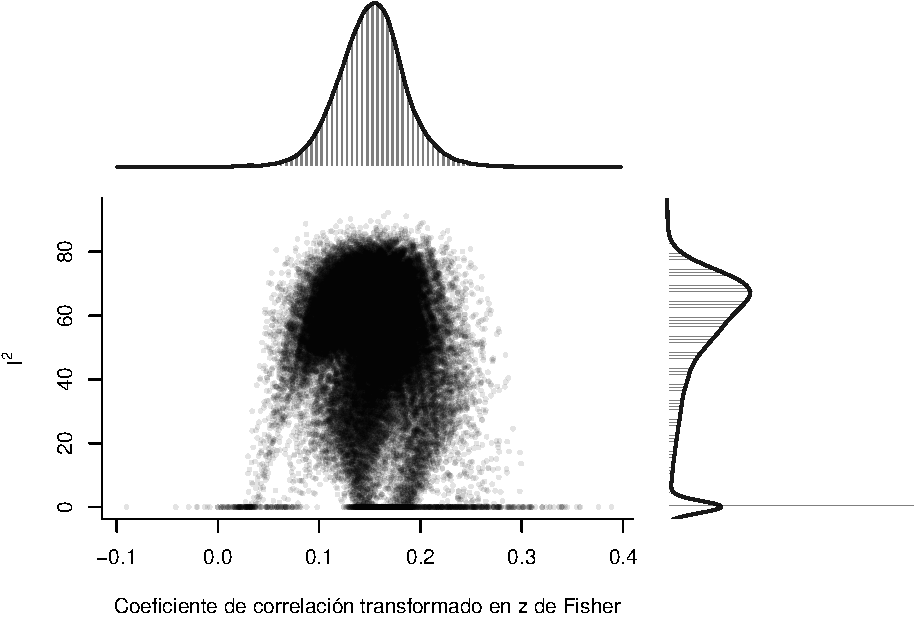
\includegraphics{Meta-analysis_files/figure-latex/gosh1-1.pdf}
\caption{\label{fig:gosh1}\emph{GOSH plot} creado con la función \href{https://www.metafor-project.org/doku.php/plots:gosh_plot}{\texttt{gosh}} del paquete \href{https://www.metafor-project.org/doku.php}{\texttt{metafor}}. Un \emph{GOSH plot} (en inglés, \emph{Graphical Display of Study Heterogeneity}) es una visualización gráfica de la heterogeneidad de todos los posibles modelos de meta-análisis ajustados a partir de todas las combinaciones posibles de estudios. Muestra los efectos estimados para cada uno de los modelos en el eje horizontal, y su respectiva heterogeneidad en el eje vertical. La distribución de los efectos (parte superior de la gráfica) y la heterogeneidade (lado derecho de la gráfica) estan representadas como densidades e histogramas.}
\end{figure}

Los tamaños del efecto que se obtienen de los estudios incluidos en un meta-análisis de correlaciones varían ampliamente, generalmente entre \emph{z} = 0.05 y \emph{z} = 0.25. Esta variación subraya cómo la elección de los estudios incluidos en el meta-análisis puede influir en la estimación del tamaño del efecto. Sin embargo, no hay un subgrupo de resultados que se distinga significativamente del resto.

Para ilustrar mejor esto, voy a manipular manualmente el tamaño de efecto de uno de los estudios. Por ejemplo, en nuestro caso, podemos cambiar el tamaño del efecto del estudio 12, que inicialmente tenía un valor \emph{z} de Fisher de 0.39, a un valor mucho mayor, de 0.70. Aunque esta base de datos alterada pierde validez para realizar cualquier análisis, nos permite visualizar el efecto de valores atípicos en una base de datos\footnote{Normalmente identificamos formalmente estudios con resultados atípicos a partir un diagnóstico de influencia (\ref{diag-inf}) y técnicas tipo \emph{leave-one-out} (sección \ref{leave-one-out}), apoyándonos informalmente en el \emph{forest plot} (sección \ref{forest-inf}) y el \emph{funnel plot} (sección \ref{funnel-inf}).}.

Para evitar afectar nuestra base de datos original, creamos una copia de los datos en un objeto llamado \texttt{dat\_mo}. Luego, utilizamos las funciones \texttt{mutate} y \texttt{replace} del paquete \texttt{dplyr} (\protect\hyperlink{ref-WickhamDplyr2021}{Wickham et al., 2021}) para cambiar los tamaños de efecto del estudio 12 en la nueva base de datos.

\begin{Shaded}
\begin{Highlighting}[]
\NormalTok{dat\_mo }\OtherTok{\textless{}{-}}\NormalTok{ dat }\SpecialCharTok{\%\textgreater{}\%}
  \FunctionTok{mutate}\NormalTok{(}\AttributeTok{yi =} \FunctionTok{replace}\NormalTok{(yi, }\AttributeTok{list =} \DecValTok{12}\NormalTok{, }\AttributeTok{values =} \FloatTok{0.7}\NormalTok{))}
\end{Highlighting}
\end{Shaded}

Para visualizar cómo el estudio 12 se convierte en un valor atípico después de la manipulación de los datos, podemos realizar un meta-análisis de la nueva base de datos alterada (\texttt{dat\_mo}) y representar los resultados en un diagrama de bosque o \emph{forest plot}. Como se puede observar en la Figura \ref{fig:for-plot-mo}, el valor atípico introducido (estudio 12) es claramente visible en el \emph{forest plot}.

\begin{Shaded}
\begin{Highlighting}[]
\NormalTok{res\_mo }\OtherTok{\textless{}{-}} \FunctionTok{rma.uni}\NormalTok{(yi, vi, }\AttributeTok{data =}\NormalTok{ dat\_mo) }
\FunctionTok{forest}\NormalTok{(res\_mo)}
\end{Highlighting}
\end{Shaded}

\begin{figure}
\centering
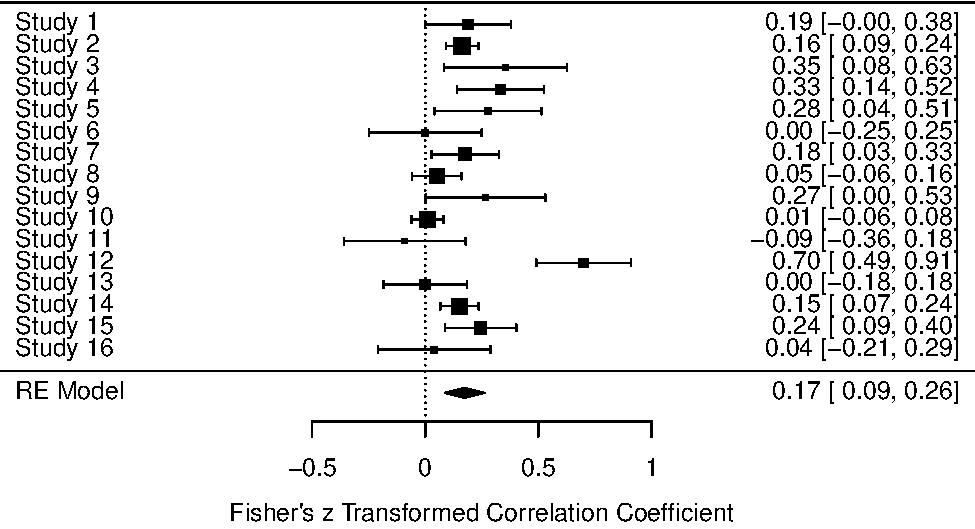
\includegraphics{Meta-analysis_files/figure-latex/for-plot-mo-1.pdf}
\caption{\label{fig:for-plot-mo}\emph{Forest plot} básico de \href{https://www.metafor-project.org/doku.php}{metafor} de la base de datos con valores atípicos introducidos manualmente para el estudio 12. Como se puede ver, este estudio tiene un tamaño de efecto muy diferente al de los demás estudios.}
\end{figure}

Hagamos el meta-análisis combinatorio con esta base de datos alterada que contiene el resultado atípico, usando de nuevo la función \texttt{plot} (Fig. \ref{fig:gosh2}) para ilustrar el resultado.

\begin{Shaded}
\begin{Highlighting}[]
\NormalTok{gp\_mo }\OtherTok{\textless{}{-}} \FunctionTok{gosh}\NormalTok{(res\_mo)}
\FunctionTok{plot}\NormalTok{(gp\_mo, }\AttributeTok{breaks =} \DecValTok{100}\NormalTok{,}
     \AttributeTok{labels =} \FunctionTok{c}\NormalTok{(}\StringTok{"Coeficiente de correlación (z de Fisher)"}\NormalTok{, }
                \FunctionTok{expression}\NormalTok{(}\FunctionTok{paste}\NormalTok{(}\StringTok{"I"}\SpecialCharTok{\^{}}\StringTok{"2"}\NormalTok{))))}
\end{Highlighting}
\end{Shaded}

\begin{figure}
\centering
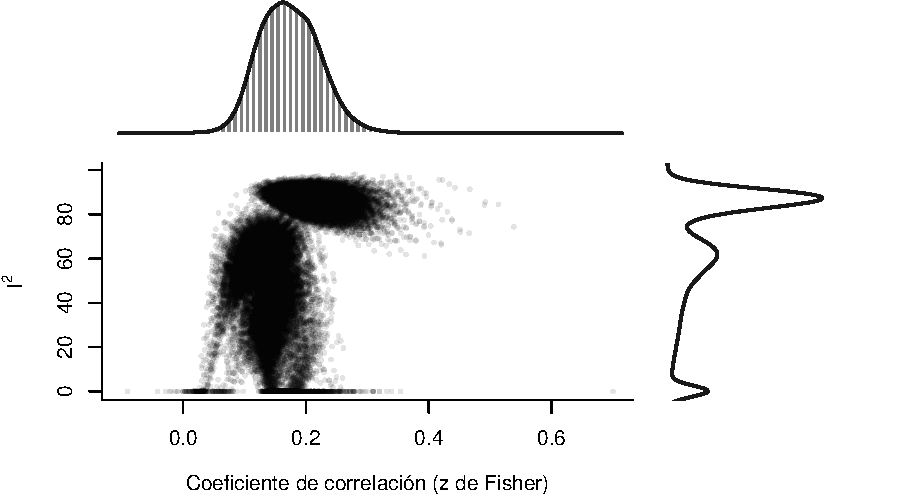
\includegraphics{Meta-analysis_files/figure-latex/gosh2-1.pdf}
\caption{\label{fig:gosh2}\emph{GOSH plot} de un meta-análisis combinatorio que contiene un estudio con resultado atípico. En la parte superior del gráfico, se observa claramente un grupo de tamaños de efecto elevados con una alta heterogeneidad.}
\end{figure}

En la parte superior de la Figura \ref{fig:gosh2} hay un claro grupo de tamaños de efecto relativamente grandes, con alta heterogeneidad. Podemos destacar específicamente los modelos del meta-análisis que incluyeron el estudio atípico con el argumento \texttt{out}:

\begin{Shaded}
\begin{Highlighting}[]
\FunctionTok{plot}\NormalTok{(gp\_mo, }\AttributeTok{breaks =} \DecValTok{100}\NormalTok{, }\AttributeTok{out =} \DecValTok{12}\NormalTok{,}
     \AttributeTok{labels =} \FunctionTok{c}\NormalTok{(}\StringTok{"Coeficiente de correlación (z de Fisher)"}\NormalTok{, }
                \FunctionTok{expression}\NormalTok{(}\FunctionTok{paste}\NormalTok{(}\StringTok{"I"}\SpecialCharTok{\^{}}\StringTok{"2"}\NormalTok{))))}
\end{Highlighting}
\end{Shaded}

\begin{figure}
\centering
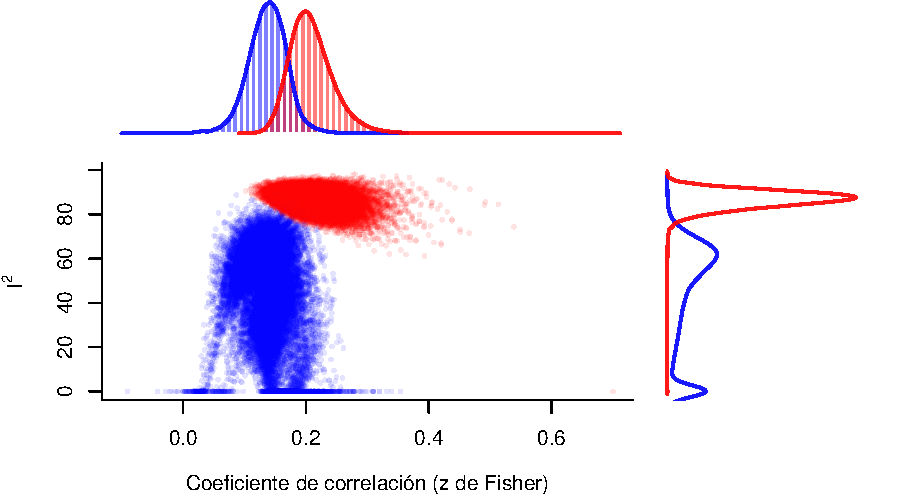
\includegraphics{Meta-analysis_files/figure-latex/gosh3-1.pdf}
\caption{\label{fig:gosh3}\emph{GOSH plot} de un meta-análisis combinatorio que contiene un estudio con resultado atípico. En este caso, a diferencia de la Figura \ref{fig:gosh2}, los resultados combinatorios que no contienen el estudio atípico están en azul, mientras que los meta-análisis que sí lo incluyen están en rojo. Los meta análisis que incluyen el estudio con un resultado atípico tienden a arrojar estimados más fuertes para la correlación, sesgando el resultado hacia valores más extremos, y son siempre almanete heterogéneos.}
\end{figure}

La inclusión del estudio 12 en los modelos de meta-análisis provoca un cambio notable en la distribución de las estimaciones del tamaño del efecto \emph{real}. Este cambio indica la importancia de considerar cuidadosamente la inclusión de cada estudio en un meta-análisis, ya que la inclusión de valores atípicos o estudios que no cumplan los criterios de calidad puede tener un impacto significativo en los resultados.

En resumen, el meta-análisis combinatorio, junto con la visualización de datos mediante gráficos \emph{GOSH}, permite demostrar cómo las opciones de análisis pueden influir en los resultados y conclusiones de un meta-análisis. Es fundamental realizar una selección cuidadosa de los estudios incluidos y llevar a cabo un análisis crítico y riguroso de los resultados obtenidos para garantizar la fiabilidad y validez del meta-análisis.

\begin{center}\rule{0.5\linewidth}{0.5pt}\end{center}

\hypertarget{met-moderation}{%
\section{Meta-análisis de correlación con moderador (meta-regresión)}\label{met-moderation}}

La inclusión de moderadores en un meta-análisis mediante una técnica llamada meta-regresión, combina principios de regresión meta-analítica y lineal. Esta técnica nos permite determinar si existe una asociación lineal entre el resultado de nuestro meta-análisis y una o más covariables; es decir, variables que pueden estar influyendo en los resultados de los estudios que estamos analizando. Al incluir estos moderadores en nuestro análisis, podemos controlar mejor la heterogeneidad y entender cómo factores específicos pueden estar afectando los resultados del meta-análisis.

Por ejemplo, en el caso de la relación entre la altura de una planta y la cantidad de luz que recibe, el tipo de suelo puede actuar como variable moderadora. Es decir, el efecto de la cantidad de luz en la altura de la planta puede ser diferente dependiendo del tipo de suelo, y estudios hechos en diferentes tipos de suelo podrían tender a encontrar resultados distintos. Por lo tanto, en este caso, el tipo de suelo actuaría como una variable moderadora de la relación entre la cantidad de luz y la altura de la planta, que deberíamos tener en cuenta en cualquier meta-análisis.

En nuestro caso, variables como la cantidad de variables controladas (\texttt{controls}), el diseño de cada estudio (\texttt{design}), la forma en la que se midieron la adherencia al tratamiento (\texttt{a\_measure}) y la escrupulosidad (\texttt{c\_measure}), la edad de los participantes (\texttt{meanage}) y/o la calidad metodológica de los estudios (\texttt{quality}), son características que podrían haber afectado el coeficiente de correlación que encontraron (todas estas variables se explican con mayor detalle en la sección \ref{variables-inf}). Por ejemplo, estudios con menor calidad metodológica podrían haber tendido a sobrestimar el efecto, encontrando correlaciones más fuertes y positivas entre escrupulosidad y adherencia al tratamiento, sesgando así nuestra estimación del efecto \emph{real}.

Los moderadores pueden ser tanto variables continuas, como categóricas, y en las siguientes secciones daré ejemplos para cada caso.

\hypertarget{ex.mod1}{%
\subsection{Ejemplo 1: Moderación de una variable continua (edad promedio de los participantes)}\label{ex.mod1}}

Primero, y como ejemplo, vamos a ver si la edad promedio de los participantes de un estudio (en nuestros datos, \texttt{meanage}) modera el resultado. Esto es importante, pues hay una enorme variación entre las edades medias de los participantes de los diferentes estudios\footnote{De hecho, mientras que en el estudio de Axelsson et al.~(2009) la edad promedio fue de 22, en el estudio de Jerant et al.~(2011) la edad promedio fue de 78.6.}, lo que podría moderar (afectar) la asociación entre escrupulosidad (\emph{conscientiousness}) y adherencia a la medicación prescrita.

Para esto, de nuevo podemos usar la función \texttt{rma} de paquete \texttt{metafor} de la misma manera que en la sección \ref{meta-cor}, pero agregando nuestra variable moderadora (\texttt{meanage}) al argumento \texttt{mods}. En este caso voy a asignar a un objeto llamado \texttt{res.modage}, para diferenciarlo del objeto \texttt{res} al que asigné el meta-análisis básico, sin moderadores.

\begin{Shaded}
\begin{Highlighting}[]
\NormalTok{res.modage }\OtherTok{\textless{}{-}} \FunctionTok{rma}\NormalTok{(}\AttributeTok{yi =}\NormalTok{ yi, }\AttributeTok{vi =}\NormalTok{ vi, }\AttributeTok{mods =} \SpecialCharTok{\textasciitilde{}}\NormalTok{meanage, }\AttributeTok{data =}\NormalTok{ dat)}
\end{Highlighting}
\end{Shaded}

Los resultados, son los siguientes:

\begin{Shaded}
\begin{Highlighting}[]
\NormalTok{res.modage}
\end{Highlighting}
\end{Shaded}

\begin{ROut}{Consola de R: Output~\thetcbcounter}
                \begin{footnotesize}
                \begin{verbatim} 
Mixed-Effects Model (k = 16; tau^2 estimator: REML)

tau^2 (estimated amount of residual heterogeneity):     0.0072 (SE = 0.0054)
tau (square root of estimated tau^2 value):             0.0846
I^2 (residual heterogeneity / unaccounted variability): 56.50%
H^2 (unaccounted variability / sampling variability):   2.30
R^2 (amount of heterogeneity accounted for):            11.76%

Test for Residual Heterogeneity:
QE(df = 14) = 30.9050, p-val = 0.0057

Test of Moderators (coefficient 2):
QM(df = 1) = 1.4286, p-val = 0.2320

Model Results:

         estimate      se     zval    pval    ci.lb   ci.ub    
intrcpt    0.2741  0.1090   2.5147  0.0119   0.0605  0.4877  * 
meanage   -0.0024  0.0020  -1.1952  0.2320  -0.0063  0.0015    

---
Signif. codes:  0 '***' 0.001 '**' 0.01 '*' 0.05 '.' 0.1 ' ' 1
 \end{verbatim}
                \end{footnotesize}
                \end{ROut}

Estos resultados tienen la misma organización que los del análisis sin moderadores (sección \ref{meta-cor}). Este resultado nos muestra que, a pesar de la gran diferencia de edad entre estudios, la edad no tiene un efecto significativo, como se puede ver en la sección ``\texttt{Test\ of\ Moderators\ (coefficient\ 2)}'' (al final nos muestra el valor \emph{p} como ``\texttt{p-val =  0.2320}''), así como los resultados para el efecto de \texttt{meanage} en la tabla \texttt{Model\ Results} (donde nos da el mismo resultado: ``\texttt{0.2320}'').

En la tabla de \texttt{Model\ results} los estimados (columna \texttt{estimate}) se pueden leer tal cual como si fueran una regresión, pero teniendo en cuenta que acá nuestra variable dependiente sería la correlación entre escrupulosidad y adherencia al tratamiento (en valores \emph{z}). Entonces, como el intercepto (\texttt{intrcpt}) tiene un valor estimado de 0.2741, para estudios con participantes que tuviesen una edad media de 0 años, se estimaría que la asociación entre escrupulosidad y adherencia al tratamiento sería de \emph{z} = 0.2741. Por su parte el efecto de la edad media (\texttt{meanage}), nuestro moderador, es de -0.0024, lo que indica que por cada año de aumento en la edad promedio de los participantes, la correlación entre escrupulosidad y adherencia disminuye \emph{z} = -0.0024. Para decirlo de manera sencilla, en nuestra muestra de estudios, la correlación entre adherencia y escrupulosidad tiende a disminuir con la edad, pero esta tendencia no es significativa.

\hypertarget{pred-mods}{%
\subsubsection{Más información e interpretación de la moderación}\label{pred-mods}}

Para más información, podemos \emph{predecir} el efecto (en este caso, la correlación entre la escrupulosidad y la adherencia a la medicación), a diferentes edades, usando la función \texttt{predict}.

En este ejemplo, como argumentos de esta función incluiré el objeto que contiene el meta-análisis con la edad como variable moderadora (\texttt{res.modage}), y los los valores para los cuales quiero saber el coeficiente de correlación predicho (argumento \texttt{newmods}); en este ejemplo voy a usar ``\texttt{seq(20,\ 80,\ by\ =\ 10)}'', lo que produce la secuencia de números de 20 a 80, cada 10 (es decir: 20, 30, 40, 50, 60, 70, 80), que serán las edades para las cuales obtendré el coeficiente de correlación estimado por el modelo\footnote{Escogí edades entre 20 y 80 como referencia, pues están cerca al rango de valores de de las edades promedio de los estudios meta-analizados (22 a 78.6), y con edades cada 10 años, para obtener un número manejable pero informativo de predicciones.}.

Adicionalmente, voy a convertir esta tabla a un objeto clase \texttt{data.frame} (usando la función \texttt{as.data.frame()}), crearé una nueva variable llamada \texttt{meanage} que contiene las edades para las cuales he calculado la predicción (\texttt{mutate(meanageage\ =\ seq(20,\ 80,\ by\ =\ 10))}\footnote{Para agregar los valores de la variable moderadora para los cuales se hace la predicción, alternativamente se puede agregar el argumento \texttt{addx\ =\ TRUE} a la función \texttt{predict} (en este caso, por ejemplo, \texttt{predict(res.modage,\ newmods\ =\ seq(20,\ 80,\ by\ =\ 10),\ addx\ =\ TRUE)}). Sin embargo, para evitar crear columnas adicionales y tener una tabla en un formato más sencillo y claro, he decidido crear la columna \texttt{meanage} manualmente. Si usara el argumento \texttt{addx\ =\ TRUE}, crearía las columnas \texttt{X.intrcpt} con el intercepto, y \texttt{X.meanage}con los valores de \texttt{meanage}.}), y reorganizado el orden de las columnas (\texttt{select(7,\ 1:6)}). Asignaré esta tabla a un objeto llamado \texttt{pred.res.modage}.

\begin{Shaded}
\begin{Highlighting}[]
\CommentTok{\# Calcular efecto ajustado para diferentes edades}
\NormalTok{pred.res.modage }\OtherTok{\textless{}{-}} \FunctionTok{predict}\NormalTok{(res.modage, }\AttributeTok{newmods =} \FunctionTok{seq}\NormalTok{(}\DecValTok{20}\NormalTok{, }\DecValTok{80}\NormalTok{, }\AttributeTok{by =} \DecValTok{10}\NormalTok{)) }\SpecialCharTok{\%\textgreater{}\%} 
  \FunctionTok{as.data.frame}\NormalTok{() }\SpecialCharTok{\%\textgreater{}\%} 
  \FunctionTok{mutate\_all}\NormalTok{(}\SpecialCharTok{\textasciitilde{}}\FunctionTok{round}\NormalTok{(., }\DecValTok{3}\NormalTok{)) }\SpecialCharTok{\%\textgreater{}\%} 
  \FunctionTok{mutate}\NormalTok{(}\AttributeTok{meanage =} \FunctionTok{seq}\NormalTok{(}\DecValTok{20}\NormalTok{, }\DecValTok{80}\NormalTok{, }\AttributeTok{by =} \DecValTok{10}\NormalTok{)) }\SpecialCharTok{\%\textgreater{}\%} 
  \FunctionTok{select}\NormalTok{(}\DecValTok{7}\NormalTok{, }\DecValTok{1}\SpecialCharTok{:}\DecValTok{6}\NormalTok{)}
\CommentTok{\# Ver la tabla}
\NormalTok{pred.res.modage}
\end{Highlighting}
\end{Shaded}

\begin{ROut}{Consola de R: Output~\thetcbcounter}
                \begin{footnotesize}
                \begin{verbatim}   meanage  pred    se  ci.lb ci.ub  pi.lb pi.ub
1      20 0.226 0.071  0.086 0.366  0.009 0.443
2      30 0.202 0.054  0.097 0.307  0.006 0.398
3      40 0.178 0.039  0.102 0.254 -0.005 0.360
4      50 0.154 0.031  0.094 0.214 -0.022 0.330
5      60 0.130 0.034  0.063 0.197 -0.049 0.309
6      70 0.106 0.047  0.013 0.198 -0.084 0.296
7      80 0.082 0.064 -0.043 0.207 -0.126 0.290
 \end{verbatim}
                \end{footnotesize}
                \end{ROut}

Con esto, el objeto \texttt{pred.res.modage}, al que he asignado esta predicción, tiene las siguientes columnas:

\begin{itemize}
\item
  \textbf{\texttt{meanage}}: edad promedio de los participantes de los estudios meta-analizados
\item
  \textbf{\texttt{pred}}: valor del efecto predicho (en este caso, coeficiente de correlación transformado en \emph{z} de Fisher), para cada edad promedio
\item
  \textbf{\texttt{se}}: error estándar (en inglés \emph{standard error}) del efecto predicho
\item
  \textbf{\texttt{ci.lb}}: límite inferior del intervalo de confianza del 95\% (en inglés \emph{confidence interval lower bound})del efecto predicho
\item
  \textbf{\texttt{ci.ub}}: límite superior del intervalo de confianza del 95\% (en inglés \emph{confidence interval upper bound}) del efecto predicho
\item
  \textbf{\texttt{pi.lb}}: límite inferior del intervalo de predicción (en inglés \emph{prediction interval lower bound}), y
\item
  \textbf{\texttt{pi.ub}}: límite superior del intervalo de predicción (en inglés \emph{prediction interval upper bound})
\end{itemize}

Las columnas \texttt{age} (edad) y \texttt{pred} (efecto predicho), nos muestran que, para estudios donde los participantes son en promedio más jóvenes, se esperaría una correlación más fuerte; por ejemplo, mientras que para estudios con personas de 20 años de edad en promedio se esperaría una correlación de \emph{z} = 0.226, para estudios con participantes con una edad promedio de 80 años, el modelo estima un efecto de \emph{z} = 0.082. En otras palabras, en nuestra muestra de estudios, la asociación entre escrupulosidad y adherencia a la medicación tiende a reducirse ligeramente con la edad promedio de la muestra.

Sin embargo, este efecto moderador de la edad \underline{no es significativo}, por lo que no tenemos evidencia suficiente para inferir que se da más allá de nuestra muestra de estudios.

\hypertarget{meta-scatter}{%
\paragraph{\texorpdfstring{\emph{Meta-Analytic Scatter Plot} (Gráfico de dispersión meta-analítico)}{Meta-Analytic Scatter Plot (Gráfico de dispersión meta-analítico)}}\label{meta-scatter}}

Alternativamente, cuando tenemos un modelo con moderador, también podemos ver la asociación entre la variable moderadora, y el efecto de cada estudio meta-analizado, a modo de regresión. La función \texttt{regplot} hace precisamente esto (Fig. \ref{fig:reg-plot1}).

\begin{Shaded}
\begin{Highlighting}[]
\FunctionTok{regplot}\NormalTok{(res.modage,}
        \AttributeTok{ylab =} \StringTok{"Coeficiente de correlación (z de Fisher)"}\NormalTok{,}
        \AttributeTok{xlab =} \StringTok{"Edad promedio de muestra"}\NormalTok{)}
\end{Highlighting}
\end{Shaded}

\begin{figure}
\centering
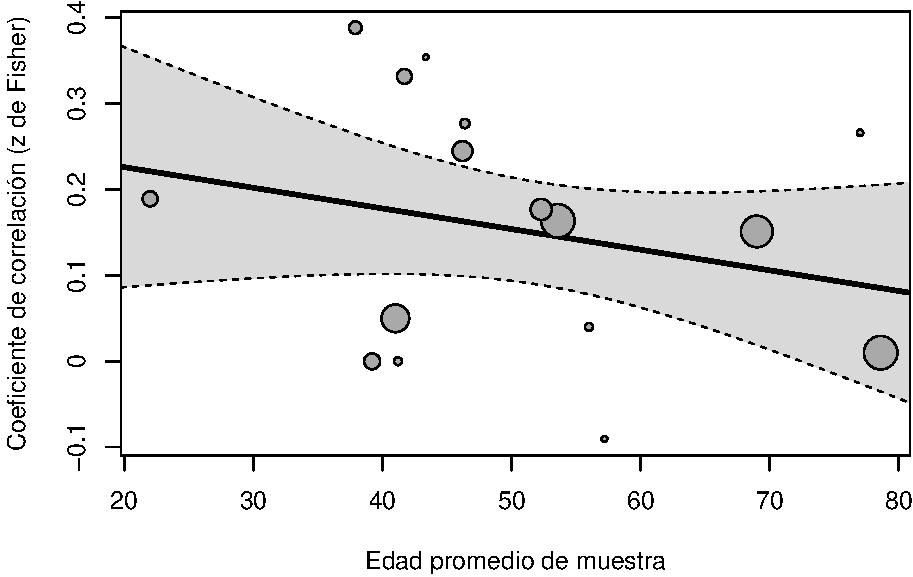
\includegraphics{Meta-analysis_files/figure-latex/reg-plot1-1.pdf}
\caption{\label{fig:reg-plot1}Gráfico de dispersión meta-analítico (\emph{Meta-Analytic Scatter Plot}). El tamaño de los puntos es proporcional al peso que recibieron los estudios en el meta-análisis (puntos más grandes para los estudios con más peso, pues tienen un tamaño de muestra mayor y con un menor error estimado). La línea negra representa el efecto previsto en función del predictor (en este caso \texttt{meanage}, edad promedio), que por supuesto coincide con las predicciones del objeto \texttt{pred.res.modage} (Output 11, en la sección \ref{pred-mods}); la banda gris demilitada por líneas punteadas representa el intervalo de confianza del 95\%.}
\end{figure}

\hypertarget{plot-mod}{%
\subsubsection{\texorpdfstring{\emph{Forest plot} y \emph{funnel plot}}{Forest plot y funnel plot}}\label{plot-mod}}

Por supuesto, de estos resultados también puedo crear \emph{forest plots} y \emph{funnel plots}, siguiendo los ejemplos y código de la sección \ref{meta-cor}. Para el \emph{forest plot}, hago a continuación un ejemplo anotado y mejorado\footnote{La función \href{https://cran.r-project.org/web/packages/metaviz/vignettes/metaviz.html\#creating-forest-plots-with-function-viz_forest}{\texttt{viz\_forest}} del paquete \href{https://cran.r-project.org/web/packages/metaviz/vignettes/metaviz.html}{\texttt{metaviz}} no puede crear un \emph{forest plot} de un meta-análisis ajustado con \texttt{metafor} cuando este modelo contiene variables moderadoras continuas, o cuando tiene como variable moderadora más de una variable categórica. En otras palabras, sólo podrá hacer el \emph{forest plot} si nuestro meta-análisis no tiene moderadores, o tiene un único moderador categórico. Como en este ejemplo nuestro moderador es una variable continua, no es posible usar esta función.} (Fig. \ref{fig:for-plot-mod1}, con un código similar al usado como ejemplo en la Fig. \ref{fig:for-plot2}). Sin embargo, es importante tener en cuenta que esta opción no creará un resumen del meta-análisis, ya que no tenemos un solo efecto \emph{real} estimado como producto del meta-análisis.

\begin{Shaded}
\begin{Highlighting}[]
\CommentTok{\# forest plot con anotaciones adicionales}
\FunctionTok{forest}\NormalTok{(res.modage,  }\AttributeTok{cex =} \FloatTok{0.75}\NormalTok{, }\AttributeTok{xlim =} \FunctionTok{c}\NormalTok{(}\SpecialCharTok{{-}}\FloatTok{1.6}\NormalTok{, }\FloatTok{1.6}\NormalTok{),}
       \AttributeTok{slab =} \FunctionTok{paste}\NormalTok{(dat}\SpecialCharTok{$}\NormalTok{authors, dat}\SpecialCharTok{$}\NormalTok{year, }\AttributeTok{sep =} \StringTok{", "}\NormalTok{),}
       \AttributeTok{showweights =} \ConstantTok{TRUE}\NormalTok{,}
       \AttributeTok{xlab =} \StringTok{"Coeficiente de correlación (z de Fisher)"}\NormalTok{,}
       \AttributeTok{digits =} \FunctionTok{c}\NormalTok{(}\DecValTok{2}\NormalTok{,3L))}
\CommentTok{\# agregar encabezados a las columnas (valores de X y Y deben ser ajustados)}
\FunctionTok{par}\NormalTok{(}\AttributeTok{cex =} \FloatTok{0.8}\NormalTok{, }\AttributeTok{font =} \DecValTok{2}\NormalTok{)}
\FunctionTok{text}\NormalTok{(}\AttributeTok{x =} \SpecialCharTok{{-}}\FloatTok{1.6}\NormalTok{, }\AttributeTok{y =} \DecValTok{18}\NormalTok{, }\AttributeTok{labels =} \StringTok{"Autor(es), Año"}\NormalTok{, }\AttributeTok{pos =} \DecValTok{4}\NormalTok{)}
\FunctionTok{text}\NormalTok{(}\AttributeTok{x =} \DecValTok{0}\NormalTok{, }\AttributeTok{y =} \DecValTok{18}\NormalTok{, }\AttributeTok{labels =} \StringTok{"Efecto e IC"}\NormalTok{, }\AttributeTok{pos =} \DecValTok{4}\NormalTok{)}
\FunctionTok{text}\NormalTok{(}\AttributeTok{x =} \DecValTok{1}\NormalTok{, }\AttributeTok{y =} \DecValTok{18}\NormalTok{, }\AttributeTok{labels =} \StringTok{"Peso"}\NormalTok{, }\AttributeTok{pos =} \DecValTok{2}\NormalTok{)}
\FunctionTok{text}\NormalTok{(}\AttributeTok{x =} \FloatTok{1.6}\NormalTok{, }\AttributeTok{y =} \DecValTok{18}\NormalTok{, }\AttributeTok{labels =} \StringTok{"Corr. [95\% IC]"}\NormalTok{, }\AttributeTok{pos =} \DecValTok{2}\NormalTok{)}
\end{Highlighting}
\end{Shaded}

\begin{figure}
\centering
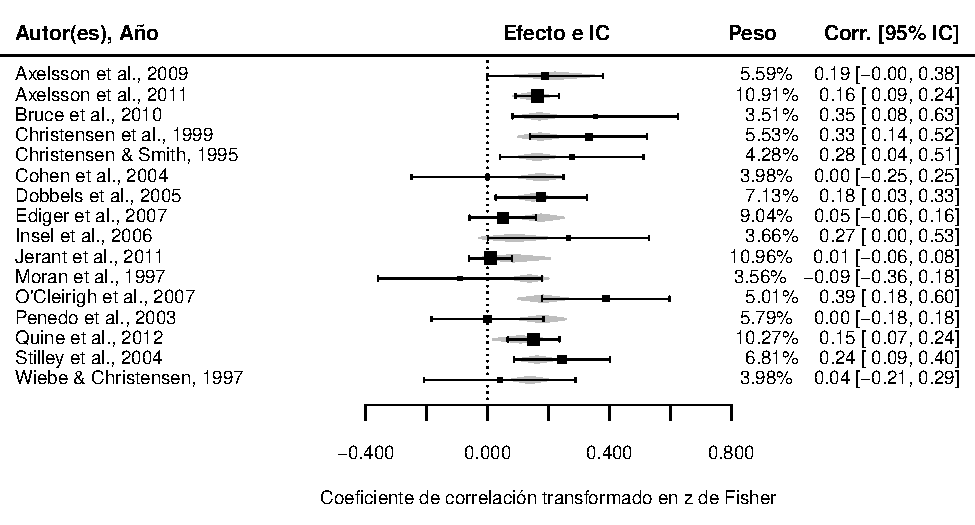
\includegraphics{Meta-analysis_files/figure-latex/for-plot-mod1-1.pdf}
\caption{\label{fig:for-plot-mod1}\emph{Forest plot} básico de \href{https://www.metafor-project.org/doku.php}{metafor}, para un meta-análisis incluyendo la edad promedio de los participantes como moderador. En la ilustración gráfica, además de los efectos originales, se puede ver el efecto de cada estudio estimado cuando se incluye el moderador como polígonos (diamantes) de color gris. Sin embargo, ya no obtenemos una fila al final representando el efecto promediado del meta-análisis, ya que no tenemos un solo efecto.}
\end{figure}

De manera similar, podemos obtener un \emph{funnel plot} de nuestro meta-análisis con moderador. Sin embargo, tanto el paquete \texttt{weightr} como el paquete \texttt{metafor} tienen funciones llamadas \texttt{funnel}, lo que puede crear un conflicto. Para evitar esto, podemos explícitamente pedir a R que use la función \texttt{funnel} del paquete \texttt{metafor} con el comando \texttt{metafor::funnel}:

\begin{Shaded}
\begin{Highlighting}[]
\NormalTok{metafor}\SpecialCharTok{::}\FunctionTok{funnel}\NormalTok{(res.modage, }\AttributeTok{xlab =} \StringTok{"Valor residual"}\NormalTok{, }\AttributeTok{ylab =} \StringTok{"Error estándar"}\NormalTok{)}
\end{Highlighting}
\end{Shaded}

\begin{figure}
\centering
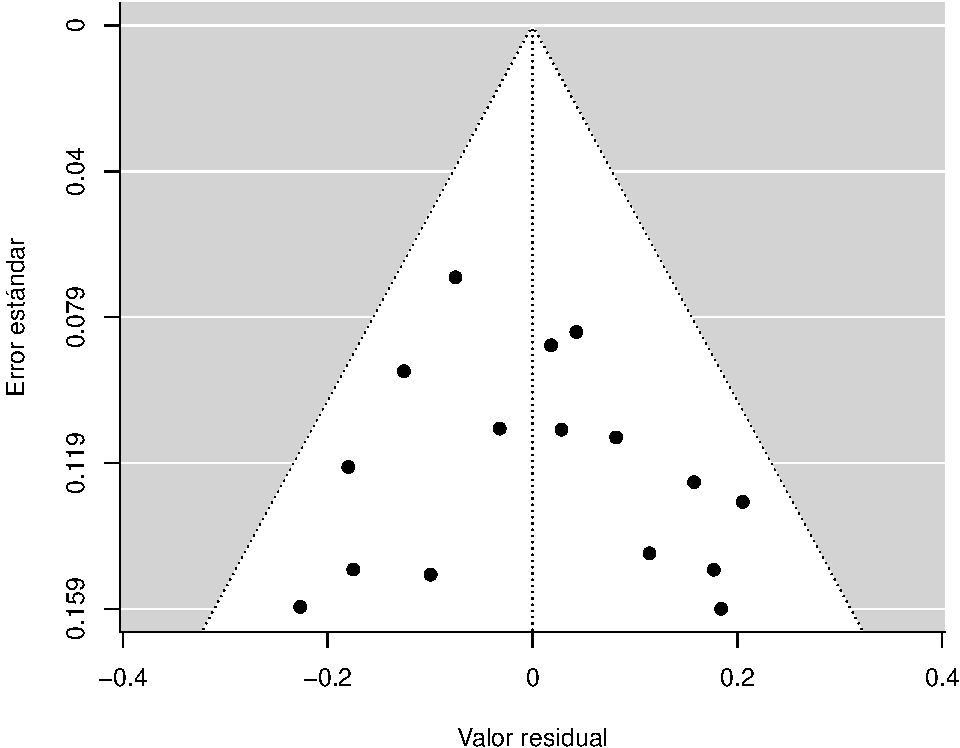
\includegraphics{Meta-analysis_files/figure-latex/funnel-plot-mod1-1.pdf}
\caption{\label{fig:funnel-plot-mod1}\emph{Funnel plot} básico de \href{https://www.metafor-project.org/doku.php}{metafor}, para un meta-análisis incluyendo la edad promedio de los participantes como moderador, y con títulos de los ejes en español. La línea punteada vertical representa el efecto meta-analizado que hemos encontrado, así que podemos ver los estudios que encontraron un efecto mayor (derecha de la línea punteada) o menor (izquierda) de éste.}
\end{figure}

Este \emph{funnel plot} (Fig. \ref{fig:funnel-plot1}), a diferencia los los anteriores, nos muestra los valores residuales de cada estudio en vez de los coeficientes de correlación (transformados a \(z\) de Fisher). Es decir, nos muestra qué tanto se aleja cada estudio del resultado de nuestro meta-análisis, que tiene un valor residual de 0 (pues no se aleja de sí mismo).

\hypertarget{reporte-cont}{%
\subsubsection{Reporte del meta-análisis con moderador continuo}\label{reporte-cont}}

Por supuesto, al igual que como se explica en la sección \ref{heterog-inf}, también podemos estimar intervalos de confianza de las medidas de heterogeneidad, con la función \texttt{confint(res.modage)}. Incluyendo esos intervalos de confianza el modelo se podría resumir, por ejemplo, así:

\begin{tcolorbox}[enhanced,attach boxed title to top center={yshift=-3mm,yshifttext=-1mm},
  colback=iacol!5!white,colframe=iacol!75!white,colbacktitle=iacol,
  title=Ejemplo de reporte con moderador continuo,fonttitle=\bfseries, parbox=false,
  boxed title style={size=small,colframe=iacol} ]
  
Dado que hay una considerable variación en la edad media de los participantes entre los estudios incluídos (con un rango entre 22 y 78.6), volvimos a ajustar el mismo meta-análisis, pero incluyendo la edad media de los participantes de cada estudio como variable moderadora. Esta meta-regresión reveló que, aunque en los estudios icluídos la asociación entre escrupulosidad y adherencia disminuye al aumentar la edad media de las muestras, esta moderación no es significativa (intercepto: $z$ ± $se$ = 0.27 ± 0.11, IC 95\% [0.06, 0.49]; $Z$ = 2.51, $p$ = .012; edad promedio: $z$ ± $se$ = -0.002 ± 0.002, IC 95\% [-0.006, 0.002]; $Z$ = -1.195, $Q$(1) = 1.429,   $p$ = .232). 

Adicionalmente, la heterogeneidad moderada y significatica se mantuvo, incluso al incluir este moderador ($\tau^2$ ± $se$ =  0.0072 ± 0.0054, IC 95\% [0.0010, 0.0403]; $\tau$ = 0.0846, IC 95\% [0.0315, 0.2007]; $Q$(14) =  30.91, $p$ = .006; $I^2$ = 56.50\%, IC 95\% [15.24\%, 87.97\%]). Por esto, no podemos inferir que la edad promedio de las muestras tenga un efecto en la estimación de la asociación entre escrupulosidad y adherencia al tratamiento.  

\end{tcolorbox}

Por supuesto, este resultado está pensado acá para ser reportado tras el reporte del meta-análisis básico (ejemplos en las secciones \ref{reporte1} y \ref{reporte2}).

De nuevo, ten en cuenta que siempre es buena idea citar tablas y figuras relevantes junto al reporte de los resultados que ilustran, pues esto facilitará la comunicación de resultados complejos. En este caso, yo citaría el gráfico de dispersión meta-analítico (\emph{Meta-Analytic Scatter Plot}; sección \ref{meta-scatter}) al presentar los resultados de la edad promedio, y el \emph{forest plot} y el \emph{funnel plot} de este meta-análisis con moderador (sección \ref{plot-mod}) al hablar de heterogeneidad.

Aunque estoy siendo extremadamente exhaustivo en la manera de reportar toda la información, hay diferentes formas de reportar tus resultados. Puedes por supuesto usar ejemplos de artículos que reporten meta-análisis para usarlos como modelo; por ejemplo, Salsman et al. (\protect\hyperlink{ref-salsmanMetaanalyticApproachExamining2015}{2015}) y Shi et al. (\protect\hyperlink{ref-shiCorrelationAdherenceRates2010}{2010}) hacen reportes distintos pero claros, y el estudio de Hidalgo-Fuentes (\protect\hyperlink{ref-hidalgo-fuentesUsoProblematicoInternet2022}{2022}) es un ejemplo sencillo del reporte de un meta-análisis de correlación, con y sin moderador, en español.

\hypertarget{ejemplo-2-moderaciuxf3n-de-una-variable-categuxf3rica-controles-usados-en-cada-estudio-meta-analizado}{%
\subsection{Ejemplo 2: Moderación de una variable categórica (controles usados en cada estudio meta-analizado)}\label{ejemplo-2-moderaciuxf3n-de-una-variable-categuxf3rica-controles-usados-en-cada-estudio-meta-analizado}}

Como segundo ejemplo, voy a mirar si el hecho de que los estudios tengan variables que fueron controladas, modera la asociación entre escrupulosidad (\emph{conscientiousness}) y adherencia a la medicación prescrita. Siguiendo los mismos pasos, voy hacer éste análisis, pero voy a asignar este meta-análisis a un objeto llamado \texttt{res.contr}.

\begin{Shaded}
\begin{Highlighting}[]
\NormalTok{res.contr }\OtherTok{\textless{}{-}} \FunctionTok{rma}\NormalTok{(}\AttributeTok{yi =}\NormalTok{ yi, }\AttributeTok{vi =}\NormalTok{ vi, }\AttributeTok{mods =} \SpecialCharTok{\textasciitilde{}}\NormalTok{controls, }\AttributeTok{data =}\NormalTok{ dat)}
\NormalTok{res.contr}
\end{Highlighting}
\end{Shaded}

\begin{ROut}{Consola de R: Output~\thetcbcounter}
                \begin{footnotesize}
                \begin{verbatim} 
Mixed-Effects Model (k = 16; tau^2 estimator: REML)

tau^2 (estimated amount of residual heterogeneity):     0.0000 (SE = 0.0015)
tau (square root of estimated tau^2 value):             0.0002
I^2 (residual heterogeneity / unaccounted variability): 0.00%
H^2 (unaccounted variability / sampling variability):   1.00
R^2 (amount of heterogeneity accounted for):            100.00%

Test for Residual Heterogeneity:
QE(df = 14) = 18.0370, p-val = 0.2051

Test of Moderators (coefficient 2):
QM(df = 1) = 20.1221, p-val < .0001

Model Results:

                  estimate      se     zval    pval    ci.lb    ci.ub      
intrcpt             0.1788  0.0208   8.6044  <.0001   0.1380   0.2195  *** 
controlsmultiple   -0.1621  0.0361  -4.4858  <.0001  -0.2329  -0.0913  *** 

---
Signif. codes:  0 '***' 0.001 '**' 0.01 '*' 0.05 '.' 0.1 ' ' 1
 \end{verbatim}
                \end{footnotesize}
                \end{ROut}

En éste caso, a diferencia del ejemplo de moderación anteriores, la variable moderadora (\texttt{controls}) sí tiene un efecto significativo, como se puede ver en el ``\texttt{Test\ of\ Moderators\ (coefficient\ 2)}'' y en la columna \texttt{pval} para el efecto de \texttt{controlsmultiple} (\textless.0001), sí como en los asteriscos que aparecen al final de esa fila (\texttt{***}).

De nuevo, en la tabla de \texttt{Model\ results} los estimados (columna \texttt{estimate}) se pueden leer tal cual como si fueran una regresión. Sin embargo es importante tener en cuenta que, dado que nuestra variable moderadora es categórica, el intercepto acá será en valor estimado de la correlación para el primer nivel (o categoría) de nuestra variable moderadora. Si recuerdas, como se explica en la sección \ref{variables-inf} la variable que estamos usando como moderadora, \texttt{controls} contiene información de si cada estudio no controló ninguna variable (\texttt{none}), o controló múltiples variables (\texttt{multiple}). Es decir, es una variable categórica con 2 niveles (\texttt{none}, \texttt{multiple}).

Entonces, como el intercepto (\texttt{intrcpt}) tiene un valor estimado de 0.1788, se estima que la asociación entre escrupulosidad y adherencia al tratamiento fue de \emph{z} = 0.1788 para estudios que no controlaron ninguna variable. Después, frente al efecto de nuestro moderador (\texttt{controlsmultiple}, que pone de manera conjunta la variable \texttt{controls} más el nivel \texttt{multiple}), nos da un estimado de -0.1621, lo que quiere decir que la correlación disminuye \emph{z} = -0.1621 cuando se trata de estudios que controlaron múltiples variables, \underline{con relación al intercepto} (\texttt{none}, en nuestro caso). De manera concreta, el modelo estimó una correlación de \emph{z} = 0.1788 para estudios que no controlaron ninguna variable, y una correlación de \emph{z} = 0.0167 (o, lo que es lo mismo, 0.1788 - 0.1621) cuando los estudios usaron varios controles.

\hypertarget{pred-mods2}{%
\subsubsection{Más información e interpretación de la moderación}\label{pred-mods2}}

\begin{Shaded}
\begin{Highlighting}[]
\NormalTok{pred.res.contr }\OtherTok{\textless{}{-}} \FunctionTok{predict}\NormalTok{(res.contr, }\AttributeTok{newmods =} \FunctionTok{c}\NormalTok{(}\DecValTok{0}\NormalTok{, }\DecValTok{1}\NormalTok{)) }\SpecialCharTok{\%\textgreater{}\%} 
  \FunctionTok{as.data.frame}\NormalTok{() }\SpecialCharTok{\%\textgreater{}\%} 
  \FunctionTok{mutate\_all}\NormalTok{(}\SpecialCharTok{\textasciitilde{}}\FunctionTok{round}\NormalTok{(., }\DecValTok{3}\NormalTok{)) }\SpecialCharTok{\%\textgreater{}\%}
  \FunctionTok{mutate}\NormalTok{(}\AttributeTok{controls =} \FunctionTok{levels}\NormalTok{(dat}\SpecialCharTok{$}\NormalTok{controls)) }\SpecialCharTok{\%\textgreater{}\%} 
  \FunctionTok{rename}\NormalTok{(}\AttributeTok{yi =}\NormalTok{ pred) }\SpecialCharTok{\%\textgreater{}\%} 
  \FunctionTok{select}\NormalTok{(}\DecValTok{7}\NormalTok{, }\DecValTok{1}\SpecialCharTok{:}\DecValTok{6}\NormalTok{)}
\NormalTok{pred.res.contr}
\end{Highlighting}
\end{Shaded}

\begin{ROut}{Consola de R: Output~\thetcbcounter}
                \begin{footnotesize}
                \begin{verbatim}   controls    yi    se  ci.lb ci.ub  pi.lb pi.ub
1     none 0.179 0.021  0.138 0.219  0.138 0.219
2 multiple 0.017 0.030 -0.041 0.075 -0.041 0.075
 \end{verbatim}
                \end{footnotesize}
                \end{ROut}

\hypertarget{meta-scatter2}{%
\paragraph{\texorpdfstring{\emph{Meta-Analytic Scatter Plot} (Gráfico de dispersión meta-analítico)}{Meta-Analytic Scatter Plot (Gráfico de dispersión meta-analítico)}}\label{meta-scatter2}}

Al igual que en el ejemplo de meta-análisis con moderación de una variable continua (sección @ref(ex.mod1)), es posible hacer un gráfico de dispersión meta-analítico (\emph{meta-analytic scatter plot}) usando la función \texttt{regplot} del paquete \texttt{metafor}. Sin embargo, dado que la variable moderadora es categórica, el modelo genera variables \emph{dummy} asignando valores de 0 y 1 a los niveles de esta variable (en este caso, 0 = ningún control; 1 = múltiples controles). Por esto, en el ejemplo a continuación agregué a la descripción del eje \(X\) esta información.

\begin{Shaded}
\begin{Highlighting}[]
\FunctionTok{regplot}\NormalTok{(res.contr,}
        \AttributeTok{ylab =} \StringTok{"Coeficiente de correlación (z de Fisher)"}\NormalTok{,}
        \AttributeTok{xlab =} \StringTok{"Controles (0 = ninguno; 1 = múltiples)"}\NormalTok{)}
\end{Highlighting}
\end{Shaded}

\begin{figure}
\centering
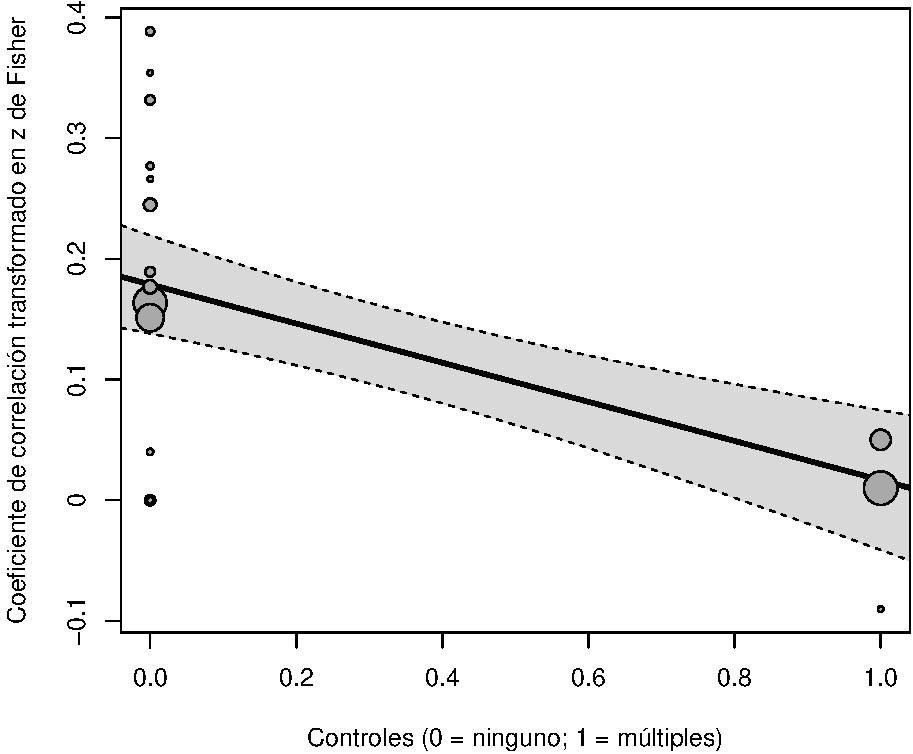
\includegraphics{Meta-analysis_files/figure-latex/reg-plot2-1.pdf}
\caption{\label{fig:reg-plot2}Gráfico de dispersión meta-analítico (\emph{Meta-Analytic Scatter Plot}) básico de \href{https://www.metafor-project.org/doku.php}{metafor} creado con la función \texttt{regplot}. El tamaño de los puntos es proporcional al peso que recibieron los estudios en el meta-análisis (puntos más grandes para los estudios con más peso, pues tienen un tamaño de muestra mayor y con un menor error estimado). La línea negra representa el efecto previsto en función del predictor (en este caso \texttt{controls}, controles). La banda gris demilimata por líneas punteadas representa el intervalo de confianza del 95\%. Dado que la variable moderadora es categórica, el modelo genera variables \emph{dummy} asignando valores de 0 y 1 a los niveles de esta variable (en este caso, 0 = ningúun control; 1 = múltiples controles), tal y como se describe en el eje \emph{X}. Para una versión más apropiada, ver Figura \ref{fig:reg-plot3}.}
\end{figure}

Aunque la Figura \ref{fig:reg-plot2} presenta información correcta, tal vez no es la más adecuada ni la más clara cuando se trata de representar meta-análisis con moderadores categóricos. Por ejemplo, a pesar de que nuestro moderador es un factor (controles) con dos niveles (ninguno, múltiples), en el eje \(X\) se representa como una variable continua con valores entre 0 y 1, que además tiene valores intermedios (0.2, 2.4, 0.6, 0.8) que en nuestro caso no tienen sentido.

Sin embargo, de manera un poco más \emph{artesanal}, es posible crear una versión más adecuada usando, por ejemplo, \texttt{ggplot2}. El código siguiente permite crear una figura mucho más adecuada usando éste paquete.

\begin{Shaded}
\begin{Highlighting}[]
\CommentTok{\# Definir base de datos, así como ejes X (controls) y Y (yi)}
\FunctionTok{ggplot}\NormalTok{(dat, }\FunctionTok{aes}\NormalTok{(}\AttributeTok{x =}\NormalTok{ controls, }\AttributeTok{y =}\NormalTok{ yi)) }\SpecialCharTok{+}
  \CommentTok{\# Agregar puntos para cada estudio, con tamaño y color según tamaño de muestra (ni)}
  \FunctionTok{geom\_point}\NormalTok{(}\FunctionTok{aes}\NormalTok{(}\AttributeTok{size =}\NormalTok{ ni, }\AttributeTok{color =}\NormalTok{ ni),}
             \AttributeTok{alpha =} \FloatTok{0.5}\NormalTok{) }\SpecialCharTok{+}
  \CommentTok{\# Definir escala de colores}
  \FunctionTok{scale\_colour\_gradient}\NormalTok{(}\AttributeTok{low =} \StringTok{"red"}\NormalTok{, }\AttributeTok{high =} \StringTok{"blue"}\NormalTok{) }\SpecialCharTok{+}
  \CommentTok{\# Definir rango de tamaño de los puntos}
  \FunctionTok{scale\_size\_continuous}\NormalTok{(}\AttributeTok{range =} \FunctionTok{c}\NormalTok{(}\DecValTok{1}\NormalTok{, }\DecValTok{10}\NormalTok{)) }\SpecialCharTok{+}
  \CommentTok{\# Combinar colores y tamaños de puntos en una sola leyenda}
  \FunctionTok{guides}\NormalTok{(}\AttributeTok{color =} \FunctionTok{guide\_legend}\NormalTok{(), }\AttributeTok{size =} \FunctionTok{guide\_legend}\NormalTok{()) }\SpecialCharTok{+}
  \CommentTok{\# Traducir etiquetas del eje X en español}
  \FunctionTok{scale\_x\_discrete}\NormalTok{(}\AttributeTok{labels=}\FunctionTok{c}\NormalTok{(}\StringTok{"none"} \OtherTok{=} \StringTok{"Ninguno"}\NormalTok{, }\StringTok{"multiple"} \OtherTok{=} \StringTok{"Múltiples"}\NormalTok{)) }\SpecialCharTok{+}
  \CommentTok{\# Cambiar títulos de ejes a español}
  \FunctionTok{labs}\NormalTok{(}\AttributeTok{x =} \StringTok{"Controles"}\NormalTok{, }
       \AttributeTok{y =} \StringTok{"Coeficiente de correlación (z de Fisher)"}\NormalTok{) }\SpecialCharTok{+}
  \CommentTok{\# Agregar barras de error para cada categoría, con base en predicción hecha en sección 4.2.1}
  \FunctionTok{geom\_errorbar}\NormalTok{(}\AttributeTok{data =}\NormalTok{ pred.res.contr,}
                \AttributeTok{mapping =} \FunctionTok{aes}\NormalTok{(}\AttributeTok{ymin =}\NormalTok{ ci.lb, }\AttributeTok{ymax =}\NormalTok{ ci.ub),}
                \AttributeTok{width =} \FloatTok{0.1}\NormalTok{, }\AttributeTok{color =} \StringTok{"black"}\NormalTok{) }\SpecialCharTok{+}
  \CommentTok{\# Agregar puntos blancos representando predicción para cada categoría hecha en sección 4.2.1}
  \FunctionTok{geom\_point}\NormalTok{(}\AttributeTok{data =}\NormalTok{ pred.res.contr,}
             \AttributeTok{shape =} \DecValTok{21}\NormalTok{, }\AttributeTok{size =} \DecValTok{3}\NormalTok{, }\AttributeTok{color =} \StringTok{"black"}\NormalTok{, }\AttributeTok{fill =} \StringTok{"white"}\NormalTok{) }\SpecialCharTok{+}
  \CommentTok{\# Cambiar título de leyenda}
  \FunctionTok{labs}\NormalTok{(}\AttributeTok{color =} \StringTok{"Tamaño de }\SpecialCharTok{\textbackslash{}n}\StringTok{muestra"}\NormalTok{, }\AttributeTok{size =} \StringTok{"Tamaño de }\SpecialCharTok{\textbackslash{}n}\StringTok{muestra"}\NormalTok{) }\CommentTok{\# "\textbackslash{}n" para salto de línea}
\end{Highlighting}
\end{Shaded}

El código anterior puede verse algo confuso para quien no haya usado \texttt{ggplot2} antes. Por esto, he agregado anotaciones, función por función, para ayudar a su interpretación\footnote{Debido a sus enormes y numerosas posibilidades, \texttt{ggplot2} es quizás la opción más poderosa para hacer gráficos estadísticos en R; por esto explicar sus bases supera por mucho el alcance de esta guía, y posiblemente requeriría múltiples tutoriales independientes. Sin embargo, hay gran cantidad de opciones disponibles en internet. Por ejemplo, puedes leer este \href{https://rpubs.com/anlope10/562981}{tutorial} (\protect\hyperlink{ref-lopezpenarandaTutorialGgplot22019}{López Peñaranda, 2019}) o ver este \href{https://youtu.be/BUzTAr_QqKs}{video} (\protect\hyperlink{ref-datademiaAprendeGgplot22018}{Datademia, 2018}).}. Este código produce la Figura \ref{fig:reg-plot3}.

\begin{figure}
\centering
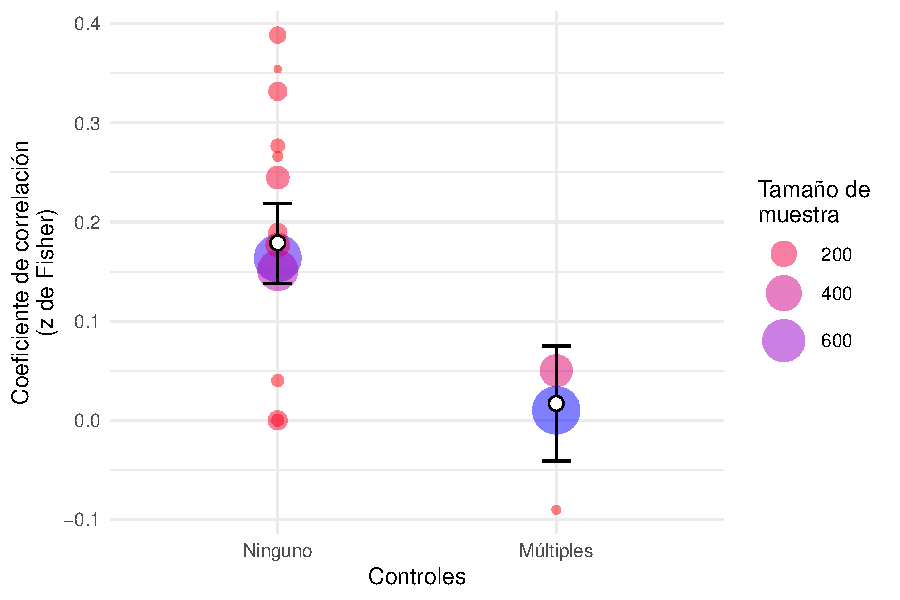
\includegraphics{Meta-analysis_files/figure-latex/reg-plot3-1.pdf}
\caption{\label{fig:reg-plot3}Gráfico de dispersión meta-analítico (\emph{Meta-Analytic Scatter Plot}) creado manualmente con \href{https://ggplot2.tidyverse.org/}{ggplot2} para hacer una mejor representación de un moderador categírico. Los puntos de colores representan el coeficiente de correlación en función de la presencia o ausencia de controles. El tamaño de los puntos es proporcional al tamaño de muestra de los estudios inluidos en el meta-análisis (puntos más grandes y azules para los estudios con mayor tamaño de muestra). Los puntos blancos superpuetos representan el efecto estimado para cada categoría, y las barras de error representan los intervalos de confianza del 95\%.}
\end{figure}

\hypertarget{plot-mod2}{%
\subsubsection{\texorpdfstring{\emph{Forest plot} y \emph{funnel plot}}{Forest plot y funnel plot}}\label{plot-mod2}}

Por supuesto, \emph{forest plots} y \emph{funnel plots} pueden ser creados, tal y como describí en la sección \ref{plot-mod}. Para el \emph{forest plots} podríamos usar el siguiente código:

\begin{Shaded}
\begin{Highlighting}[]
\CommentTok{\# forest plot con anotaciones adicionales}
\FunctionTok{forest}\NormalTok{(res.contr,  }\AttributeTok{cex =} \FloatTok{0.75}\NormalTok{, }\AttributeTok{xlim =} \FunctionTok{c}\NormalTok{(}\SpecialCharTok{{-}}\FloatTok{1.6}\NormalTok{, }\FloatTok{1.6}\NormalTok{),}
       \AttributeTok{slab =} \FunctionTok{paste}\NormalTok{(dat}\SpecialCharTok{$}\NormalTok{authors, dat}\SpecialCharTok{$}\NormalTok{year, }\AttributeTok{sep =} \StringTok{", "}\NormalTok{),}
       \AttributeTok{showweights =} \ConstantTok{TRUE}\NormalTok{,}
       \AttributeTok{xlab =} \StringTok{"Coeficiente de correlación (z de Fisher)"}\NormalTok{,}
       \AttributeTok{digits =} \FunctionTok{c}\NormalTok{(}\DecValTok{2}\NormalTok{,3L))}
\CommentTok{\# agregar encabezados a las columnas (valores de X y Y deben ser ajustados)}
\FunctionTok{par}\NormalTok{(}\AttributeTok{cex =} \FloatTok{0.8}\NormalTok{, }\AttributeTok{font =} \DecValTok{2}\NormalTok{)}
\FunctionTok{text}\NormalTok{(}\AttributeTok{x =} \SpecialCharTok{{-}}\FloatTok{1.6}\NormalTok{, }\AttributeTok{y =} \DecValTok{18}\NormalTok{, }\AttributeTok{labels =} \StringTok{"Autor(es), Año"}\NormalTok{, }\AttributeTok{pos =} \DecValTok{4}\NormalTok{)}
\FunctionTok{text}\NormalTok{(}\AttributeTok{x =} \DecValTok{0}\NormalTok{, }\AttributeTok{y =} \DecValTok{18}\NormalTok{, }\AttributeTok{labels =} \StringTok{"Efecto e IC"}\NormalTok{, }\AttributeTok{pos =} \DecValTok{4}\NormalTok{)}
\FunctionTok{text}\NormalTok{(}\AttributeTok{x =} \DecValTok{1}\NormalTok{, }\AttributeTok{y =} \DecValTok{18}\NormalTok{, }\AttributeTok{labels =} \StringTok{"Peso"}\NormalTok{, }\AttributeTok{pos =} \DecValTok{2}\NormalTok{)}
\FunctionTok{text}\NormalTok{(}\AttributeTok{x =} \FloatTok{1.6}\NormalTok{, }\AttributeTok{y =} \DecValTok{18}\NormalTok{, }\AttributeTok{labels =} \StringTok{"Corr. [95\% IC]"}\NormalTok{, }\AttributeTok{pos =} \DecValTok{2}\NormalTok{)}
\end{Highlighting}
\end{Shaded}

Ese código produce esta Figura \ref{fig:for-plot-mod2}.

\begin{figure}
\centering
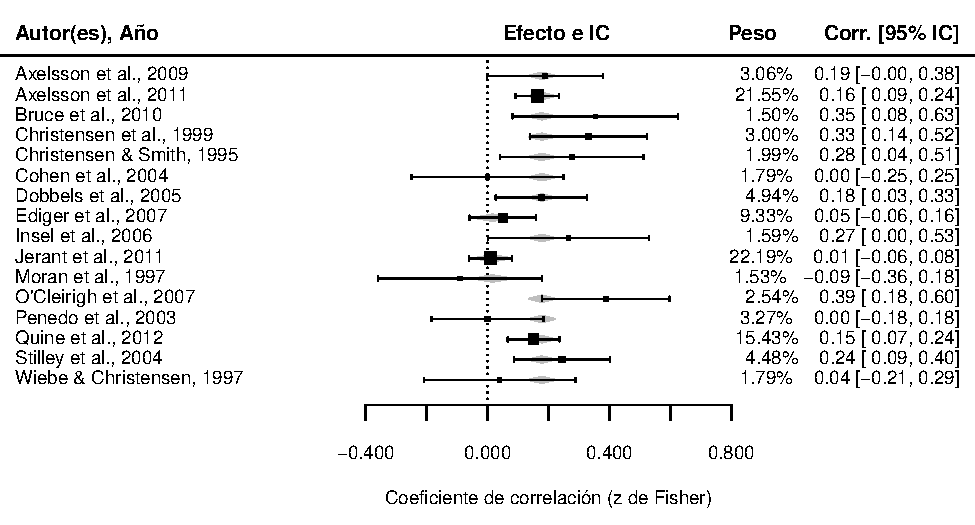
\includegraphics{Meta-analysis_files/figure-latex/for-plot-mod2-1.pdf}
\caption{\label{fig:for-plot-mod2}\emph{Forest plot} básico de \href{https://www.metafor-project.org/doku.php}{metafor}, para un meta-análisis incluyendo como moderador si los estudios incluyeron múltiples controles esyadísticos o ninguno. En la ilustración gráfica, además de los efectos originales, se puede ver el efecto de cada estudio estimado cuando se incluye el moderador como polígonos (diamantes) de color gris. Sin embargo, ya no obtenemos una fila al final representando el efecto promediado del meta-análisis, ya que no tenemos un solo efecto.}
\end{figure}

De manera similar, podemos obtener un \emph{funnel plot}, pero recuerda que dado que tanto el paquete \texttt{weightr} como el paquete \texttt{metafor} tienen funciones llamadas \texttt{funnel}debemos pedirle a R explícitamente que use la función \texttt{funnel} del paquete \texttt{metafor} con el comando \texttt{metafor::funnel}.
Este \emph{funnel plot}, nos mostrará los valores residuales de cada estudio (es decir, qué tanto se alejan del resultado de nuestro meta-análisis, que tiene un valor residual de 0; Fig. \ref{fig:funnel-plot1}), en vez de los coeficientes de correlación (transformados a \(z\) de Fisher).

Adicionalmente no olvides que este \textbf{funnel plot} nos mostrará los valores residuales de cada estudio, dado que se trata de un meta-análisis con moderador, tal como lo expliqué en la sección \ref{plot-mod}.

\begin{Shaded}
\begin{Highlighting}[]
\NormalTok{metafor}\SpecialCharTok{::}\FunctionTok{funnel}\NormalTok{(res.contr,}
                \AttributeTok{xlab =} \StringTok{"Valor residual"}\NormalTok{,}
                \AttributeTok{ylab =} \StringTok{"Error estándar"}\NormalTok{)}
\end{Highlighting}
\end{Shaded}

Esto producirá la siguiente Figura \ref{fig:funnel-plot2}.

\begin{figure}
\centering
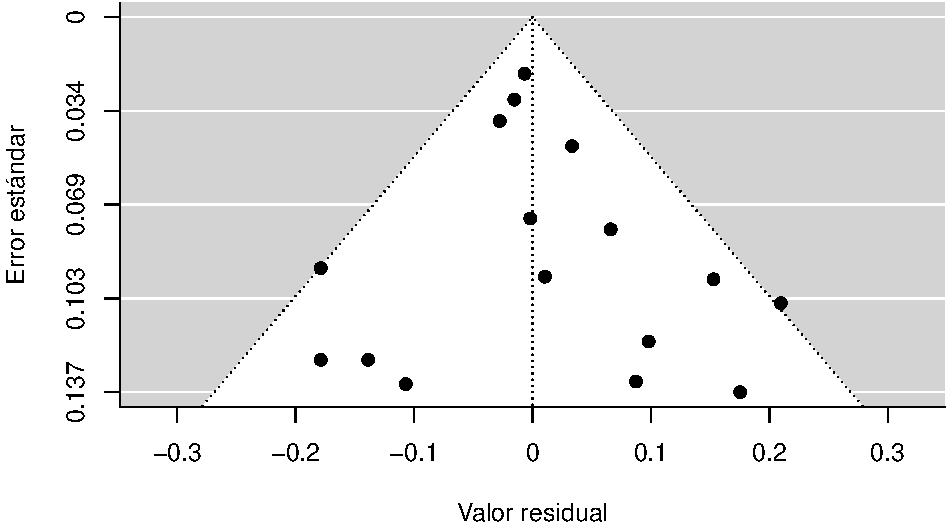
\includegraphics{Meta-analysis_files/figure-latex/funnel-plot-mod2-1.pdf}
\caption{\label{fig:funnel-plot-mod2}\emph{Funnel plot} básico de \href{https://www.metafor-project.org/doku.php}{metafor}, para un meta-análisis incluyendo como moderador si los estudios incluyeron múltiples controles esyadísticos o ninguno. La línea punteada vertical representa el efecto meta-analizado que hemos encontrado, así que podemos ver los estudios que encontraron un efecto mayor (derecha de la línea punteada) o menor (izquierda) de éste.}
\end{figure}

\hypertarget{reporte-cat}{%
\subsubsection{Reporte del meta-análisis con moderador categórico}\label{reporte-cat}}

De nuevo, y tal como lo hicimos en la sección \ref{heterog-inf} y en la sección \ref{reporte-cont}, es posible estimar intervalos de confianza de las medidas de heterogeneidad. Para ello, en este caso usamos la función \texttt{confint(res.contr)}. El reporte incluyendo esta información podría ser algo como esto:

\begin{tcolorbox}[enhanced,attach boxed title to top center={yshift=-3mm,yshifttext=-1mm},
  colback=iacol!5!white,colframe=iacol!75!white,colbacktitle=iacol,
  title=Ejemplo de reporte con moderador categórico,fonttitle=\bfseries, parbox=false,
  boxed title style={size=small,colframe=iacol} ]
  
Dado que hay estudios que controlaron variables y otros que no controlaron ninguna, ajustamos de nuevo el meta-análisis, pero incluyendo este factor como variable moderadora. Al incluir la variable moderadora de controles en el meta-análisis, se encontró que esta tuvo un efecto significativo en la estimación de la correlación entre la escrupulosidad y la adherencia al tratamiento ($Q$(1) = 20.122, $p$ < .0001). De hecho, los estudios que no incorporaron controles estimaron una asociación más alta ($z$ ± $se$ = 0.179 ± 0.021, IC 95\% [0.138, 0.219]) que los estudios que incluyeron múltiples controles ($z$ ± $se$ = 0.017 ± 0.030, IC 95\% [-0.041, 0.075]).

Al incluir esta variable moderadora, se redujo enormemente la heterogeneidad entre los estudios ($\tau^2$ ± $se$ =  0.00 ± 0.0015, IC 95\% [0.0000, 0.0244]; $\tau$ = 0.0002, IC 95\% [0.000, 0.1562]; $Q$(14) = 18.037, $p$ = .205; $I^2$ = 0.00\%, IC 95\% [0.00\%, 80.96\%]), lo que indica que la heterogeneidad original se debía en gran parte a las diferencias metodológicas entre los estudios.  

\end{tcolorbox}

Como antes, es importante tener en cuenta que este resultado debería ser reportado después del meta-análisis básico, como se muestra en las secciones \ref{reporte1} y \ref{reporte2}. Además, al presentar los resultados, te recomiendo citar las tablas y figuras pertinentes que los ilustren, ya que esto puede facilitar la comunicación de resultados complejos. En particular, al reportar los resultados de la moderación, se podría hacer referencia al gráfico de dispersión meta-analítico (sección \ref{meta-scatter2}). Asimismo, para hablar de la heterogeneidad, se podría citar el \emph{forest plot} y el \emph{funnel plot} correspondientes a este meta-análisis con moderador (sección \ref{plot-mod2}).

Aunque es importante proporcionar información detallada y exhaustiva en el reporte de los resultados de un meta-análisis, existen diferentes formas de hacerlo. Una recomendación es utilizar como modelos algunos artículos que hayan reportado meta-análisis previamente. Por ejemplo, el trabajo de Hidalgo-Fuentes (\protect\hyperlink{ref-hidalgo-fuentesUsoProblematicoInternet2022}{2022}) es un ejemplo sencillo de cómo reportar un meta-análisis de correlación, tanto con como sin moderador, en español. Poor otro lado, los estudios de Salsman et al. (\protect\hyperlink{ref-salsmanMetaanalyticApproachExamining2015}{2015}) y Shi et al. (\protect\hyperlink{ref-shiCorrelationAdherenceRates2010}{2010}) presentan reportes de manera distinta pero clara (en inglés).

\begin{center}\rule{0.5\linewidth}{0.5pt}\end{center}

\hypertarget{recomendaciones-generales}{%
\section{Recomendaciones generales}\label{recomendaciones-generales}}

Hacer un meta-análisis de correlación en R no es necesariamente complejo, pero podría requerir acciones que pueden parecer algo laberínticas. Sin embargo, la confiabilidad del resultado que obtengas, dependerá de varios aspectos. Por esto, la realización de un meta-análisis requiere una comprensión de los métodos estadísticos involucrados, la selección y evaluación de estudios relevantes, y la identificación y consideración de posibles fuentes de heterogeneidad y sesgo.

\hypertarget{pasos-para-hacer-tu-meta-anuxe1lisis}{%
\subsection{Pasos para hacer tu meta-análisis}\label{pasos-para-hacer-tu-meta-anuxe1lisis}}

Primero, debes tener hacer una selección de artículos buena y no sesgada\footnote{Para esto existen varias guías, e incluso la \emph{Declaración PRISMA} que está diseñada para abordar los problemas en la publicación de revisiones sistemáticas y meta-análisis (para información en español, ver e.g., \protect\hyperlink{ref-huttonExtensionDeclaracionPRISMA2016}{Hutton et al., 2016}; \protect\hyperlink{ref-pageDeclaracionPRISMA20202021}{Page et al., 2021}).

  A. Formular la pregunta de investigación clara, con base en teoría

  B. Identificar la bibliografía pertinente

  C. Extraer y consolidar los datos de los estudios (en el caso de correlaciones, cuando menos \emph{r} y \emph{n})}. Esto mínimamente incluye:

Con esto deberías ya poder hacer una base de datos para un meta-análisis de correlación simple. Mientras tengas en tu base de datos algún identificador de cada estudio, el tamaño de efecto (\emph{r}) y el tamaño de muestra (\emph{n}), tendrías todo lo necesario para hacerlo. Por ejemplo:

\begin{longtable}[]{@{}lll@{}}
\toprule()
estudio & ri & ni \\
\midrule()
\endhead
Autores (año) & 0.25 & 425 \\
Autores (año) & 0.65 & 45 \\
Autores (año) & 0.12 & 235 \\
\bottomrule()
\end{longtable}

Adicionalmente, podrías definir o extraer información de posibles variables moderadoras; por ejemplo, si los estudios se pudieran agrupar según metodología usada o población estudiada, y sospechas que estas variables afectan la correlación encontrada en cada estudio, podrías agregar esta información en una o más variables que podrías usar como moderadores.

Una vez tengas tu base de datos lista, deberías, cuando menos:

\begin{enumerate}
\def\labelenumi{\arabic{enumi}.}
\item
  Hacer el meta-análisis (sin moderador, sección \ref{meta-cor}; con moderador, sección \ref{met-moderation})

  1.1 Reportar información sobre heterogeneidad (sección \ref{heterog-inf})

  1.2 Hacer un diagnóstico de influencia (sección \ref{diag-inf}; incluir, si es posible y no tienes un número grande de estudios, un meta-análisis combinatorio, sección \ref{gosh})

  1.3 Reportar los resultados usando un \emph{forest plot} (diagrama de bosque; sección \ref{forest-inf})

  1.4 Mostrar la distribución de los resultados en un \emph{funnel plot} (diagrama de embudo; sección \ref{funnel-inf}) y estimar el sesgo de estudios pequeños (sección \ref{reg-egger})
\item
  Estimar si hay evidencia de sesgo de publicación (sección \ref{sesgo-pub})

  2.1 Puedes usar el método \emph{trim and fill} (recorte y relleno; sección \ref{trim-fill}) o, lo que es mejor, hacer una estimación del modelo de función de peso (sección \ref{vevea-hedges})
\end{enumerate}

Adicionalmente, podrías:

\begin{enumerate}
\def\labelenumi{\arabic{enumi}.}
\setcounter{enumi}{2}
\tightlist
\item
  Estimar el poder estadístico del meta-análisis y los estudios meta-analizados (sección \ref{poder-inf})
\end{enumerate}

\hypertarget{conclusiuxf3n}{%
\subsection{Conclusión}\label{conclusiuxf3n}}

Es fundamental tener en cuenta que el meta-análisis, aunque es una herramienta poderosa, no es una solución mágica para resolver los problemas de investigación. La calidad de los estudios incluidos, la heterogeneidad de los datos y otras limitaciones pueden influir en los resultados y su interpretación. En última instancia, el éxito de un meta-análisis dependerá del rigor y la transparencia del investigador o investigadora en su implementación y en la interpretación de sus resultados.

Sin embargo, si tienes en cuenta y de manera rigurosa las recomendaciones de esta guía, tendrás una base sólida para hacer y comunicar tu meta-análisis de manera transparente, sin importar los resultados obtenidos.

Lamentablemente, en el mundo hispano, especialmente en Latinoamérica, todavía se presentan importantes rezagos en la producción científica, que son resultado en parte del insuficiente apoyo gubernamental y de un sistema global que desfavorece a los países en vías de desarrollo. Sin embargo, también son producto de una falta de confianza en las capacidades propias y de ciertos déficits reales en educación.

Mi objetivo con esta guía es inspirar a investigadores hispanohablantes, ya sean establecidos o en formación, y de diversas disciplinas, a conocer los fundamentos del meta-análisis y su implementación de forma transparente. El fortalecimiento de nuestras habilidades analíticas es un paso fundamental para mejorar nuestra formación y contribuir al conocimiento global.

\begin{center}\rule{0.5\linewidth}{0.5pt}\end{center}

\hypertarget{referencias}{%
\section*{Referencias}\label{referencias}}
\addcontentsline{toc}{section}{Referencias}

\footnotesize
\begin{multicols}{2}

\hypertarget{refs}{}
\begin{CSLReferences}{1}{0}
\leavevmode\vadjust pre{\hypertarget{ref-magrittrcite}{}}%
Bache, S. M., \& Wickham, H. (2022). \emph{{magrittr}: A forward-pipe operator for {R}}. \url{https://CRAN.R-project.org/package=magrittr}

\leavevmode\vadjust pre{\hypertarget{ref-baker500ScientistsLift2016}{}}%
Baker, M. (2016). 1,500 scientists lift the lid on reproducibility. \emph{Nature News}, \emph{533}(7604), 452. \url{https://doi.org/10.1038/533452a}

\leavevmode\vadjust pre{\hypertarget{ref-BalduzziMeta2019}{}}%
Balduzzi, S., Rücker, G., \& Schwarzer, G. (2019). How to perform a meta-analysis with {R}: A practical tutorial. \emph{Evidence-Based Mental Health}, \emph{22}, 153--160. \url{https://doi.org/10.1136/ebmental-2019-300117}

\leavevmode\vadjust pre{\hypertarget{ref-belsleyRegressionDiagnosticsIdentifying1980}{}}%
Belsley, D. A., Kuh, E., \& Welsch, R. E. (1980). \emph{Regression {Diagnostics}: {Identifying Influential Data} and {Sources} of {Collinearity}}. {John Wiley \& Sons, Inc.} \url{https://doi.org/10.1002/0471725153}

\leavevmode\vadjust pre{\hypertarget{ref-borensteinIdentifyingQuantifyingHeterogeneity2009}{}}%
Borenstein, M., Hedges, L. V., Higgns, J. P. T., \& Rothstein, H. R. (2009). Identifying and {Quantifying Heterogeneity}. In \emph{Introduction to {Meta}-{Analysis}} (pp. 107--125). Wiley. \url{https://doi.org/10.1002/9780470743386.ch16}

\leavevmode\vadjust pre{\hypertarget{ref-coburnPublicationBiasFunction2015}{}}%
Coburn, K. M., \& Vevea, J. L. (2015). Publication bias as a function of study characteristics. \emph{Psychological Methods}, \emph{20}(3), 310--330. \url{https://doi.org/10.1037/met0000046}

\leavevmode\vadjust pre{\hypertarget{ref-coburnWeightr2019}{}}%
Coburn, K. M., \& Vevea, J. L. (2019). \emph{Weightr: Estimating weight-function models for publication bias}. \url{https://CRAN.R-project.org/package=weightr}

\leavevmode\vadjust pre{\hypertarget{ref-cookDetectionInfluentialObservation1977}{}}%
Cook, R. D. (1977). Detection of {Influential Observation} in {Linear Regression}. \emph{Technometrics}, \emph{19}(1), 15--18. \url{https://doi.org/10.2307/1268249}

\leavevmode\vadjust pre{\hypertarget{ref-cookResidualsInfluenceRegression1982}{}}%
Cook, R. D., \& Weisberg, S. (1982). \emph{Residuals and {Influence} in {Regression}}. {New York: Chapman and Hall}. \url{https://hdl.handle.net/11299/37076}

\leavevmode\vadjust pre{\hypertarget{ref-copasSensitivityAnalysisPublication2001}{}}%
Copas, J., \& Shi, J. Q. (2001). A sensitivity analysis for publication bias in systematic reviews. \emph{Statistical Methods in Medical Research}, \emph{10}(4), 251--265. \url{https://doi.org/10.1177/096228020101000402}

\leavevmode\vadjust pre{\hypertarget{ref-copasMetaanalysisFunnelPlots2000}{}}%
Copas, J., \& Shi, J. Q. (2000). Meta-analysis, funnel plots and sensitivity analysis. \emph{Biostatistics}, \emph{1}(3), 247--262. \url{https://doi.org/10.1093/biostatistics/1.3.247}

\leavevmode\vadjust pre{\hypertarget{ref-datademiaAprendeGgplot22018}{}}%
Datademia. (2018). \emph{Aprende {Ggplot2} en {R} \emph{{[}video{]}}}. YouTube. \url{https://youtu.be/BUzTAr_QqKs}.

\leavevmode\vadjust pre{\hypertarget{ref-duvalTrimFillMethod2005}{}}%
Duval, S. (2005). The {Trim} and {Fill Method}. In H. R. Rothstein, A. J. Sutton, \& M. Borenstein (Eds.), \emph{Publication {Bias} in {Meta-Analysis}} (pp. 127--144). {John Wiley \& Sons}. \url{https://doi.org/10.1002/0470870168.ch8}

\leavevmode\vadjust pre{\hypertarget{ref-duvalNonparametricTrimFill2000}{}}%
Duval, S., \& Tweedie, R. (2000a). A {Nonparametric} {``{Trim} and {Fill}''} {Method} of {Accounting} for {Publication Bias} in {Meta-Analysis}. \emph{Journal of the American Statistical Association}, \emph{95}(449), 89--98. \url{https://doi.org/10.1080/01621459.2000.10473905}

\leavevmode\vadjust pre{\hypertarget{ref-duvalTrimFillSimple2000}{}}%
Duval, S., \& Tweedie, R. (2000b). Trim and {Fill}: {A Simple Funnel-Plot-Based Method} of {Testing} and {Adjusting} for {Publication Bias} in {Meta-Analysis}. \emph{Biometrics}, \emph{56}(2), 455--463. \url{https://doi.org/10.1111/j.0006-341X.2000.00455.x}

\leavevmode\vadjust pre{\hypertarget{ref-eggerBiasMetaanalysisDetected1997}{}}%
Egger, M., Smith, G. D., Schneider, M., \& Minder, C. (1997). {Bias in Meta-Analysis Detected by a Simple, Graphical Test}. \emph{BMJ}, \emph{315}(7109), 629--634. \url{https://doi.org/10.1136/bmj.315.7109.629}

\leavevmode\vadjust pre{\hypertarget{ref-fisherFrequencyDistributionValues1915}{}}%
Fisher, R. A. (1915). Frequency {Distribution} of the {Values} of the {Correlation Coefficient} in {Samples} from an {Indefinitely Large Population}. \emph{Biometrika}, \emph{10}(4), 507--521. \url{https://doi.org/10.2307/2331838}

\leavevmode\vadjust pre{\hypertarget{ref-SesgoPublicacion2008}{}}%
Gómez-Restrepo, C. (2008). {Acerca del sesgo de publicación en literatura sobre antidepresivos}. \emph{Revista Colombiana de Psiquiatría}, \emph{37}(1), 8--10. \url{http://www.scielo.org.co/scielo.php?script=sci_arttext\&pid=S0034-74502008000100001}

\leavevmode\vadjust pre{\hypertarget{ref-harrer2021doing}{}}%
Harrer, M., Cuijpers, P., A, F. T., \& Ebert, D. D. (2021). \emph{{Doing Meta-Analysis With {R}: A Hands-On Guide}} (1st ed.). {Chapman \& Hall/CRC Press}. \url{https://bookdown.org/MathiasHarrer/Doing_Meta_Analysis_in_R/}

\leavevmode\vadjust pre{\hypertarget{ref-Harrer2019dmetar}{}}%
Harrer, M., Cuijpers, P., Furukawa, T., \& Ebert, D. D. (2019). \emph{{dmetar: Companion R Package For The Guide 'Doing Meta-Analysis in R'}}. \url{http://dmetar.protectlab.org/}

\leavevmode\vadjust pre{\hypertarget{ref-Henry2003}{}}%
Henry, N. W., Cohen, J., \& Cohen, P. (2003). \emph{Applied {Multiple Regression}/{Correlation Analysis} for the {Behavioral Sciences}.} (3rd ed.). {Lawrence Erlbaum Associates}. \url{https://doi.org/10.4324/9780203774441}

\leavevmode\vadjust pre{\hypertarget{ref-hidalgo-fuentesUsoProblematicoInternet2022}{}}%
Hidalgo-Fuentes, S. (2022). {Uso problemático de Internet y procrastinación en estudiantes: un meta-análisis}. \emph{European Journal of Education and Psychology}, 1--18. \url{https://doi.org/10.32457/ejep.v15i1.1815}

\leavevmode\vadjust pre{\hypertarget{ref-huttonExtensionDeclaracionPRISMA2016}{}}%
Hutton, B., Catalá-López, F., \& Moher, D. (2016). {La extensión de la declaración PRISMA para revisiones sistemáticas que incorporan metaanálisis en red: PRISMA-NMA}. \emph{Medicina Clínica}, \emph{147}(6), 262--266. \url{https://doi.org/10.1016/j.medcli.2016.02.025}

\leavevmode\vadjust pre{\hypertarget{ref-johnBigFiveTrait1999}{}}%
John, O. P., \& Srivastava, S. (1999). The {Big Five Trait} taxonomy: {History}, measurement, and theoretical perspectives. In L. A. Pervin \& O. P. John (Eds.), \emph{Handbook of personality: {Theory} and research, 2nd ed} (pp. 102--138). {Guilford Press}. \url{http://jenni.uchicago.edu/econ-psych-traits/John_Srivastava_1995_big5.pdf}

\leavevmode\vadjust pre{\hypertarget{ref-kleinManyLabsInvestigating2018}{}}%
Klein, R. A., Vianello, M., Hasselman, F., Adams, B. G., Adams, R. B., Alper, S., Aveyard, M., Axt, J. R., Babalola, M. T., Bahník, Š., Batra, R., Berkics, M., Bernstein, M. J., Berry, D. R., Bialobrzeska, O., Binan, E. D., Bocian, K., Brandt, M. J., Busching, R., \ldots{} Nosek, B. A. (2018). Many {Labs} 2: {Investigating Variation} in {Replicability Across Samples} and {Settings}. \emph{Advances in Methods and Practices in Psychological Science}, \emph{1}(4), 443--490. \url{https://doi.org/10.1177/2515245918810225}

\leavevmode\vadjust pre{\hypertarget{ref-KossmeierMetaviz}{}}%
Kossmeier, M., Tran, U. S., \& Voracek, M. (2020). \emph{{metaviz: Forest Plots, Funnel Plots, and Visual Funnel Plot Inference for Meta-Analysis}}. \url{https://CRAN.R-project.org/package=metaviz}

\leavevmode\vadjust pre{\hypertarget{ref-lakensImprovingYourStatistical2022}{}}%
Lakens, D. (2022). \emph{Improving {Your Statistical Inferences}}. \url{https://lakens.github.io/statistical_inferences/}

\leavevmode\vadjust pre{\hypertarget{ref-leongomezMetaanalysis2021}{}}%
Leongómez, J. D. (2021). \emph{Hacer meta-análisis en jamovi es muy fácil \emph{{[}video{]}}}. YouTube. \url{https://youtu.be/ntBbkOn9D_o}.

\leavevmode\vadjust pre{\hypertarget{ref-leongomezAnalisisPoderEstadistico2020}{}}%
Leongómez, J. D. (2020a). \emph{Análisis de poder estadístico y cálculo de tamaño de muestra en {R}: {Guía} práctica}. {Zenodo}. \url{https://doi.org/10.5281/zenodo.3988776}

\leavevmode\vadjust pre{\hypertarget{ref-leongomezPoderRvid2020}{}}%
Leongómez, J. D. (2020b). \emph{Poder estadístico y tamaño de muestra en {R} \emph{{[}serie de videos{]}}}. YouTube. \url{https://youtube.com/playlist?list=PLHk7UNt35ccVdyHqnQ6oXVYA6JBNFrE1x}.

\leavevmode\vadjust pre{\hypertarget{ref-lopezpenarandaTutorialGgplot22019}{}}%
López Peñaranda, A. (2019). \emph{Tutorial de ggplot2}. RPubs. \url{https://rpubs.com/anlope10/562981}.

\leavevmode\vadjust pre{\hypertarget{ref-Manterola2019}{}}%
Manterola, C., Quiroz, G., Salazar, P., \& García, N. (2019). Metodología de los tipos y diseños de estudio más frecuentemente utilizados en investigación clínica. \emph{Revista Médica Clínica Las Condes}, \emph{30}(1), 36--49. https://doi.org/\url{https://doi.org/10.1016/j.rmclc.2018.11.005}

\leavevmode\vadjust pre{\hypertarget{ref-molloy2013}{}}%
Molloy, G. J., O'Carroll, R. E., \& Ferguson, E. (2013). Conscientiousness and medication adherence: A meta-analysis. \emph{Annals of Behavioral Medicine}, \emph{47}(1), 92--101. \url{https://doi.org/10.1007/s12160-013-9524-4}

\leavevmode\vadjust pre{\hypertarget{ref-olkinGOSHGraphicalDisplay2012}{}}%
Olkin, I., Dahabreh, I. J., \& Trikalinos, T. A. (2012). {GOSH} \textendash{} a graphical display of study heterogeneity. \emph{Research Synthesis Methods}, \emph{3}(3), 214--223. \url{https://doi.org/10.1002/jrsm.1053}

\leavevmode\vadjust pre{\hypertarget{ref-pageDeclaracionPRISMA20202021}{}}%
Page, M. J., McKenzie, J. E., Bossuyt, P. M., Boutron, I., Hoffmann, T. C., Mulrow, C. D., Shamseer, L., Tetzlaff, J. M., Akl, E. A., Brennan, S. E., Chou, R., Glanville, J., Grimshaw, J. M., Hróbjartsson, A., Lalu, M. M., Li, T., Loder, E. W., Mayo-Wilson, E., McDonald, S., \ldots{} Alonso-Fernández, S. (2021). {Declaración PRISMA 2020: una guía actualizada para la publicación de revisiones sistemáticas}. \emph{Revista Española de Cardiología}, \emph{74}(9), 790--799. \url{https://doi.org/10.1016/j.recesp.2021.06.016}

\leavevmode\vadjust pre{\hypertarget{ref-quintanaOhMyGOSH2020}{}}%
Quintana, D. S. (2020). \emph{{Oh My GOSH: Calculating All Possible Meta-Analysis Study Combinations} \emph{{[}{B}log{]}}}. {Hormones, brain, and behavior.} \url{https://www.dsquintana.blog/combinatorial-meta-analysis/}

\leavevmode\vadjust pre{\hypertarget{ref-quintanaMetameta2022}{}}%
Quintana, D. S. (2022). \emph{Metameta: A suite of tools to re-evaluate published meta-analyses}. \url{https://github.com/dsquintana/metameta}

\leavevmode\vadjust pre{\hypertarget{ref-quintanaGuideMetaPower}{}}%
Quintana, D. S. (2023). A guide for calculating study-level statistical power for meta-analyses. \emph{{Advances in Methods and Practices in Psychological Science}}, \emph{6}(1), 1--18. \url{https://doi.org/10.1177/25152459221147260}

\leavevmode\vadjust pre{\hypertarget{ref-revellePsych2021}{}}%
Revelle, W. (2021). \emph{Psych: Procedures for psychological, psychometric, and personality research}. Northwestern University. \url{https://CRAN.R-project.org/package=psych}

\leavevmode\vadjust pre{\hypertarget{ref-salsmanMetaanalyticApproachExamining2015}{}}%
Salsman, J. M., Pustejovsky, J. E., Jim, H. S. L., Munoz, A. R., Merluzzi, T. V., George, L., Park, C. L., Danhauer, S. C., Sherman, A. C., Snyder, M. A., \& Fitchett, G. (2015). A meta-analytic approach to examining the correlation between religion/spirituality and mental health in cancer. \emph{Cancer}, \emph{121}(21), 3769--3778. \url{https://doi.org/10.1002/cncr.29350}

\leavevmode\vadjust pre{\hypertarget{ref-sanchez-brunoTransformacionFisherPara2005}{}}%
Sánchez-Bruno, A., \& Borges del Rosal, Á. (2005). {Transformación Z de Fisher para la determinación de intervalos de confianza del coeficiente de correlación de Pearson}. \emph{Psicothema}, \emph{17}(1), 148--153. \url{https://www.redalyc.org/articulo.oa?id=72717124}

\leavevmode\vadjust pre{\hypertarget{ref-schwarzerMetaAnalysis2015}{}}%
Schwarzer, G., Carpenter, J. R., \& Rücker, G. (2015a). \emph{Meta-{Analysis} with {R}}. {Springer International Publishing}. \url{https://doi.org/10.1007/978-3-319-21416-0}

\leavevmode\vadjust pre{\hypertarget{ref-schwarzerSmallStudyEffectsMetaAnalysis2015}{}}%
Schwarzer, G., Carpenter, J. R., \& Rücker, G. (2015b). Small-{Study Effects} in {Meta}-{Analysis}. In \emph{Meta-{Analysis} with {R}} (pp. 107--141). \url{https://doi.org/10.1007/978-3-319-21416-0_5}

\leavevmode\vadjust pre{\hypertarget{ref-schwarzerMetasensPackage}{}}%
Schwarzer, G., Carpenter, J. R., \& Rücker, G. (2023). \emph{Metasens: Statistical methods for sensitivity analysis in meta-analysis}. \url{https://CRAN.R-project.org/package=metasens}

\leavevmode\vadjust pre{\hypertarget{ref-schwarzerEmpiricalEvaluationSuggests2010}{}}%
Schwarzer, G., Carpenter, J., \& Rücker, G. (2010). Empirical evaluation suggests {Copas} selection model preferable to trim-and-fill method for selection bias in meta-analysis. \emph{Journal of Clinical Epidemiology}, \emph{63}(3), 282--288. \url{https://doi.org/10.1016/j.jclinepi.2009.05.008}

\leavevmode\vadjust pre{\hypertarget{ref-sedgwickMetaanalysesWhatHeterogeneity2015}{}}%
Sedgwick, P. (2015). Meta-analyses: What is heterogeneity? \emph{BMJ}, \emph{350}, h1435. \url{https://doi.org/10.1136/bmj.h1435}

\leavevmode\vadjust pre{\hypertarget{ref-shadishCombiningEstimatesEffect2009}{}}%
Shadish, W. R., \& Haddock, C. K. (2009). Combining estimates of effect size. In H. M. Cooper, L. V. Hedges, \& J. C. Valentine (Eds.), \emph{The handbook of research synthesis and meta-analysis} (2nd ed., pp. 257--277). {Russell Sage Foundation}.

\leavevmode\vadjust pre{\hypertarget{ref-shiTrimandfill2019}{}}%
Shi, L., \& Lin, L. (2019). The trim-and-fill method for publication bias: Practical guidelines and recommendations based on a large database of meta-analyses. \emph{Medicine}, \emph{98}(23), e15987. \url{https://doi.org/10.1097/MD.0000000000015987}

\leavevmode\vadjust pre{\hypertarget{ref-shiCorrelationAdherenceRates2010}{}}%
Shi, L., Liu, J., Fonseca, V., Walker, P., Kalsekar, A., \& Pawaskar, M. (2010). Correlation between adherence rates measured by {MEMS} and self-reported questionnaires: A meta-analysis. \emph{Health and Quality of Life Outcomes}, \emph{8}(1), 99. \url{https://doi.org/10.1186/1477-7525-8-99}

\leavevmode\vadjust pre{\hypertarget{ref-simonsohnPcurveWonYour2019}{}}%
Simonsohn, U., Nelson, L. D., \& Simmons, J. P. (2019). P-curve won't do your laundry, but it will distinguish replicable from non-replicable findings in observational research: {Comment} on {Bruns} \& {Ioannidis} (2016). \emph{PLOS ONE}, \emph{14}(3), e0213454. \url{https://doi.org/10.1371/journal.pone.0213454}

\leavevmode\vadjust pre{\hypertarget{ref-simonsohnPCurveEffectSize2014}{}}%
Simonsohn, U., Nelson, L. D., \& Simmons, J. P. (2014). P-{Curve} and {Effect Size}: {Correcting} for {Publication Bias Using Only Significant Results}. \emph{Perspectives on Psychological Science}, \emph{9}(6), 666--681. \url{https://doi.org/10.1177/1745691614553988}

\leavevmode\vadjust pre{\hypertarget{ref-sternePublicationRelatedBias2000}{}}%
Sterne, J. A. C., Gavaghan, D., \& Egger, M. (2000). Publication and related bias in meta-analysis. \emph{Journal of Clinical Epidemiology}, \emph{53}(11), 1119--1129. \url{https://doi.org/10.1016/S0895-4356(00)00242-0}

\leavevmode\vadjust pre{\hypertarget{ref-sterneRecommendationsExaminingInterpreting2011}{}}%
Sterne, J. A. C., Sutton, A. J., Ioannidis, J. P. A., Terrin, N., Jones, D. R., Lau, J., Carpenter, J., Rucker, G., Harbord, R. M., Schmid, C. H., Tetzlaff, J., Deeks, J. J., Peters, J., Macaskill, P., Schwarzer, G., Duval, S., Altman, D. G., Moher, D., \& Higgins, J. P. T. (2011). Recommendations for examining and interpreting funnel plot asymmetry in meta-analyses of randomised controlled trials. \emph{BMJ}, \emph{343}(1), d4002. \url{https://doi.org/10.1136/bmj.d4002}

\leavevmode\vadjust pre{\hypertarget{ref-veveaGeneralLinearModel1995}{}}%
Vevea, J. L., \& Hedges, L. V. (1995). A general linear model for estimating effect size in the presence of publication bias. \emph{Psychometrika}, \emph{60}(3), 419--435. \url{https://doi.org/10.1007/BF02294384}

\leavevmode\vadjust pre{\hypertarget{ref-veveaPublicationBiasResearch2005}{}}%
Vevea, J. L., \& Woods, C. M. (2005). Publication bias in research synthesis: Sensitivity analysis using a priori weight functions. \emph{Psychological Methods}, \emph{10}(4), 428--443. \url{https://doi.org/10.1037/1082-989X.10.4.428}

\leavevmode\vadjust pre{\hypertarget{ref-viechtbauer2010}{}}%
Viechtbauer, W. (2010). Conducting meta-analyses in {R} with the metafor package. \emph{Journal of Statistical Software}, \emph{36}(3). \url{https://doi.org/10.18637/jss.v036.i03}

\leavevmode\vadjust pre{\hypertarget{ref-Wickhamforcats2022}{}}%
Wickham, H. (2022). \emph{Forcats: Tools for working with categorical variables (factors)}. \url{https://CRAN.R-project.org/package=forcats}

\leavevmode\vadjust pre{\hypertarget{ref-WickhamDplyr2021}{}}%
Wickham, H., François, R., Henry, L., \& Müller, K. (2021). \emph{Dplyr: A grammar of data manipulation}. \url{https://CRAN.R-project.org/package=dplyr}

\end{CSLReferences}

\end{multicols}

\hypertarget{apuxe9ndices}{%
\section*{APÉNDICES}\label{apuxe9ndices}}
\addcontentsline{toc}{section}{APÉNDICES}

\hypertarget{appendix-apuxe9ndice}{%
\appendix}


\opensupplement
\normalsize

\hypertarget{apendice-alt}{%
\subsection*{\texorpdfstring{\emph{Apéndice A.} Alternativas a \texttt{metafor}}{Apéndice A. Alternativas a metafor}}\label{apendice-alt}}
\addcontentsline{toc}{subsection}{\emph{Apéndice A.} Alternativas a \texttt{metafor}}

A lo largo de ésta guía he usado una ruta para hacer meta-análisis que parte de objetos generados con el paquete \texttt{metafor}. Sin embargo, existen rutas alternativas para realizar meta-análisis en R. El libro \emph{Doing meta-analysis with R: a hands-on guide} (\protect\hyperlink{ref-harrer2021doing}{Harrer et al., 2021}) se acompaña del paquete \href{https://dmetar.protectlab.org/index.html}{\texttt{dmetar}} (\protect\hyperlink{ref-Harrer2019dmetar}{Harrer et al., 2019}), que contiene y explica opciones para hacer meta-análisis tanto a partir de \texttt{metafor}, como a partir de \texttt{meta} (\protect\hyperlink{ref-BalduzziMeta2019}{Balduzzi et al., 2019}; \protect\hyperlink{ref-schwarzerMetaAnalysis2015}{Schwarzer et al., 2015a}).

Los objetos generados por \texttt{meta} al realizar un meta-análisis permiten hacer otros análisis como \emph{risk of bias} (riesgo de sesgo), inferencia multi-modelo, detección de \emph{outliers} (valores atípicos), y \emph{p-curve} o curva de valores \(p\) (\protect\hyperlink{ref-simonsohnPcurveWonYour2019}{Simonsohn et al., 2019}, \protect\hyperlink{ref-simonsohnPCurveEffectSize2014}{2014}), y permiten hacer gráficos distintos. Para una guía resumida y concreta (en inglés) de estas opciones, recomiendo ver el sitio web del paquete \href{http://dmetar.protectlab.org/}{\texttt{dmetar}}, y en especial la página \href{https://dmetar.protectlab.org/articles/dmetar.html}{\emph{Get Started}}.

\hypertarget{p-curve}{%
\subsubsection*{\texorpdfstring{\emph{A1.} Ejemplo: curva de valores \(p\) (\emph{p-curve})}{A1. Ejemplo: curva de valores p (p-curve)}}\label{p-curve}}
\addcontentsline{toc}{subsubsection}{\emph{A1.} Ejemplo: curva de valores \(p\) (\emph{p-curve})}

Como ejemplo puntual, la curva de valores \(p\) (en inglés \emph{p-curve}) de nuestro meta-análisis se podría hacer tras ajustar el modelo con la función \texttt{metacor} (que hace meta-análisis de correlaciones) del paquete \texttt{meta} (\protect\hyperlink{ref-BalduzziMeta2019}{Balduzzi et al., 2019}; \protect\hyperlink{ref-schwarzerMetaAnalysis2015}{Schwarzer et al., 2015a}). Para este ejemplo asignaré el resultado a un objeto que llamaré \texttt{res.meta}.

\begin{Shaded}
\begin{Highlighting}[]
\FunctionTok{library}\NormalTok{(meta)}
\NormalTok{res.meta }\OtherTok{\textless{}{-}} \FunctionTok{metacor}\NormalTok{(}\AttributeTok{cor =}\NormalTok{ yi, }\AttributeTok{n =}\NormalTok{ ni, }
                    \AttributeTok{studlab =} \FunctionTok{paste}\NormalTok{(dat}\SpecialCharTok{$}\NormalTok{authors, dat}\SpecialCharTok{$}\NormalTok{year, }\AttributeTok{sep =} \StringTok{", "}\NormalTok{), }
                    \AttributeTok{data =}\NormalTok{ dat, }\AttributeTok{sm =} \StringTok{"ZCOR"}\NormalTok{)}
\end{Highlighting}
\end{Shaded}

El objeto resultante (\texttt{res.meta}) puede usarse directamente como argumento a la función \texttt{pcurve} del paquete \href{http://dmetar.protectlab.org/}{\texttt{dmetar}}, para obtener una gráfica con la curva de valores \(p\) (\emph{p-curve}). Es importante tener en cuenta que, al menos por ahora, \texttt{dmetar} debe instalarse desde GitHub tal como \texttt{metameta} (en este caso, con el comando \texttt{devtools::install\_github("MathiasHarrer/dmetar")}).

\begin{Shaded}
\begin{Highlighting}[]
\FunctionTok{library}\NormalTok{(dmetar)}
\FunctionTok{pcurve}\NormalTok{(res.meta)}
\end{Highlighting}
\end{Shaded}

\begin{figure}

{\centering 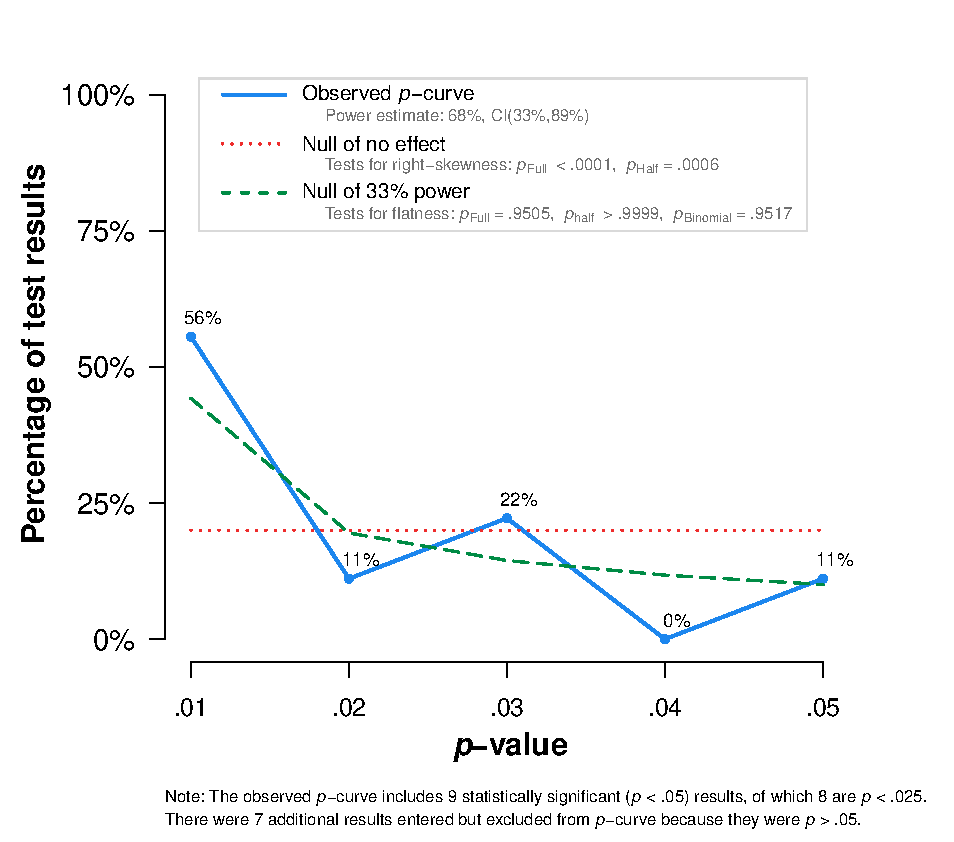
\includegraphics[width=300px]{images/pcurve} 

}

\caption{Curva de valores $p$ (\textit{p-curve}) creada con \href{http://dmetar.protectlab.org/}{\texttt{dmetar}}. Para una entender una curva de valores $p$, su relevancia y su interpretación, sugiero leer Simonsohn et al. (2019, 2014), o ver el sitio web del paquete \texttt{dmetar}: \href{http://dmetar.protectlab.org/}{http://dmetar.protectlab.org/}.}\label{fig:pcurve-plot}
\end{figure}

La función \texttt{pcurve} produce varios elementos relacionados la curva de valores \(p\), incluyendo la Figura \ref{fig:pcurve-plot} que resume éste análisis.

\hypertarget{paquetes-cit}{%
\subsection*{\texorpdfstring{\emph{Apéndice B.} Citas y referencias de paquetes de R}{Apéndice B. Citas y referencias de paquetes de R}}\label{paquetes-cit}}
\addcontentsline{toc}{subsection}{\emph{Apéndice B.} Citas y referencias de paquetes de R}

Por supuesto, los paquetes de R que usemos deben ser citados. Una manera fácil de encontrar la cita que los autores de un paquete quieren que usemos, es la función \texttt{citation} en R. Simplemente debemos usar esta función, agregando como argumento el nombre del paquete que queremos citar entre comillas. Esto nos dará la referencia en un formato estándar, así como como en un formato \texttt{BibTex} que puede ser usado en documentos \LaTeX, o por muchos gestores de referencia como \href{https://www.zotero.org/}{Zotero}. Alternativamente, el formato formato \texttt{BibTex} nos permite saber los campos como autores, título y demás, si vamos a crear las citas y referencias manualmente, o incluso crear referencias en diversos estilos usando, por ejemplo, \href{https://asouqi.github.io/bibtex-converter/}{Online Bibtex Converter}.

Como ejemplo, en ésta guía usé \texttt{dplyr} (\protect\hyperlink{ref-WickhamDplyr2021}{Wickham et al., 2021}) para manipular los datos. Usando la función \texttt{citation}:

\begin{Shaded}
\begin{Highlighting}[]
\FunctionTok{citation}\NormalTok{(}\StringTok{"dplyr"}\NormalTok{)}
\end{Highlighting}
\end{Shaded}

Obtengo esta información sobre ese paquete:

\begin{ROut}{Consola de R: Output~\thetcbcounter}
                \begin{footnotesize}
                \begin{verbatim} 
To cite package 'dplyr' in publications use:

  Wickham H, François R, Henry L, Müller K, Vaughan D (2023). _dplyr: A
  Grammar of Data Manipulation_. R package version 1.1.1,
  <https://CRAN.R-project.org/package=dplyr>.

A BibTeX entry for LaTeX users is

  @Manual{,
    title = {dplyr: A Grammar of Data Manipulation},
    author = {Hadley Wickham and Romain François and Lionel Henry and Kirill Müller and Davis Vaughan},
    year = {2023},
    note = {R package version 1.1.1},
    url = {https://CRAN.R-project.org/package=dplyr},
  }
 \end{verbatim}
                \end{footnotesize}
                \end{ROut}

\hypertarget{paquetes-list}{%
\subsection*{\texorpdfstring{\emph{Apéndice C.} Paquetes de R usados para crear este documento}{Apéndice C. Paquetes de R usados para crear este documento}}\label{paquetes-list}}
\addcontentsline{toc}{subsection}{\emph{Apéndice C.} Paquetes de R usados para crear este documento}

\textbf{R version 4.2.3 (2023-03-15 ucrt)}

\textbf{Platform:} x86\_64-w64-mingw32/x64 (64-bit)

\textbf{attached base packages:}
\emph{stats}, \emph{graphics}, \emph{grDevices}, \emph{utils}, \emph{datasets}, \emph{methods} and \emph{base}

\textbf{other attached packages:}
\emph{meta(v.6.2-1)}, \emph{metameta(v.0.1.1)}, \emph{weightr(v.2.0.2)}, \emph{scales(v.1.2.1)}, \emph{metaviz(v.0.3.1)}, \emph{tidyquant(v.1.0.6)}, \emph{quantmod(v.0.4.20)}, \emph{TTR(v.0.24.3)}, \emph{PerformanceAnalytics(v.2.0.4)}, \emph{xts(v.0.13.0)}, \emph{zoo(v.1.8-11)}, \emph{psych(v.2.3.3)}, \emph{kableExtra(v.1.3.4)}, \emph{ggpubr(v.0.6.0)}, \emph{lubridate(v.1.9.2)}, \emph{forcats(v.1.0.0)}, \emph{stringr(v.1.5.0)}, \emph{dplyr(v.1.1.1)}, \emph{purrr(v.1.0.1)}, \emph{readr(v.2.1.4)}, \emph{tidyr(v.1.3.0)}, \emph{tibble(v.3.2.1)}, \emph{ggplot2(v.3.4.1)}, \emph{tidyverse(v.2.0.0)}, \emph{metafor(v.4.0-0)}, \emph{numDeriv(v.2016.8-1.1)}, \emph{metadat(v.1.2-0)}, \emph{Matrix(v.1.5-3)}, \emph{robumeta(v.2.1)} and \emph{knitr(v.1.42)}

\textbf{loaded via a namespace (and not attached):}
\emph{nlme(v.3.1-162)}, \emph{webshot(v.0.5.4)}, \emph{RColorBrewer(v.1.1-3)}, \emph{httr(v.1.4.5)}, \emph{tools(v.4.2.3)}, \emph{backports(v.1.4.1)}, \emph{utf8(v.1.2.3)}, \emph{R6(v.2.5.1)}, \emph{mgcv(v.1.8-42)}, \emph{colorspace(v.2.1-0)}, \emph{withr(v.2.5.0)}, \emph{tidyselect(v.1.2.0)}, \emph{gridExtra(v.2.3)}, \emph{mnormt(v.2.1.1)}, \emph{curl(v.5.0.0)}, \emph{compiler(v.4.2.3)}, \emph{cli(v.3.6.1)}, \emph{rvest(v.1.0.3)}, \emph{xml2(v.1.3.3)}, \emph{labeling(v.0.4.2)}, \emph{bookdown(v.0.33)}, \emph{quadprog(v.1.5-8)}, \emph{systemfonts(v.1.0.4)}, \emph{digest(v.0.6.31)}, \emph{minqa(v.1.2.5)}, \emph{rmarkdown(v.2.21)}, \emph{svglite(v.2.1.1)}, \emph{pkgconfig(v.2.0.3)}, \emph{htmltools(v.0.5.5)}, \emph{lme4(v.1.1-32)}, \emph{fastmap(v.1.1.1)}, \emph{highr(v.0.10)}, \emph{ggthemes(v.4.2.4)}, \emph{rlang(v.1.1.0)}, \emph{rstudioapi(v.0.14)}, \emph{generics(v.0.1.3)}, \emph{farver(v.2.1.1)}, \emph{jsonlite(v.1.8.4)}, \emph{car(v.3.1-1)}, \emph{magrittr(v.2.0.3)}, \emph{Rcpp(v.1.0.10)}, \emph{Quandl(v.2.11.0)}, \emph{munsell(v.0.5.0)}, \emph{fansi(v.1.0.4)}, \emph{abind(v.1.4-5)}, \emph{lifecycle(v.1.0.3)}, \emph{stringi(v.1.7.12)}, \emph{yaml(v.2.3.7)}, \emph{CompQuadForm(v.1.4.3)}, \emph{carData(v.3.0-5)}, \emph{MASS(v.7.3-58.2)}, \emph{mathjaxr(v.1.6-0)}, \emph{grid(v.4.2.3)}, \emph{parallel(v.4.2.3)}, \emph{lattice(v.0.20-45)}, \emph{cowplot(v.1.1.1)}, \emph{splines(v.4.2.3)}, \emph{pander(v.0.6.5)}, \emph{hms(v.1.1.3)}, \emph{pillar(v.1.9.0)}, \emph{boot(v.1.3-28.1)}, \emph{ggsignif(v.0.6.4)}, \emph{glue(v.1.6.2)}, \emph{evaluate(v.0.20)}, \emph{nloptr(v.2.0.3)}, \emph{vctrs(v.0.6.1)}, \emph{tzdb(v.0.3.0)}, \emph{gtable(v.0.3.3)}, \emph{xfun(v.0.38)}, \emph{broom(v.1.0.4)}, \emph{rstatix(v.0.7.2)}, \emph{viridisLite(v.0.4.1)} and \emph{timechange(v.0.2.0)}

\end{document}
